% Este fichero es parte del N�mero 3 de la Revista Occam's Razor
% Revista Occam's Razor N�mero 3
%
% (c)  2007, 2008, 2009, The Occam's Razor Team
%
% Esta obra est� bajo una licencia Reconocimiento 3.0 Espa�a de
% Creative Commons. Para ver una copia de esta licencia, visite
% http://creativecommons.org/licenses/by/3.0/es/ o envie una carta a
% Creative Commons, 171 Second Street, Suite 300, San Francisco,
% California 94105, USA. 


\documentclass[10pt,a4paper,twoside]{article}

% Paquetes... probablemente alguno no sea necesario
% 

\usepackage[latin1]{inputenc}
\usepackage[greek,spanish]{babel}  % S�mbolo del euro
\usepackage{graphicx}
\usepackage{a4,fancyhdr, multicol}
\usepackage{float}
\usepackage{pdftricks}
\usepackage{pstricks}
\usepackage{color}
\usepackage{pst-plot}
\usepackage{pst-eps}
\usepackage{wrapfig}
\usepackage{eso-pic}
\usepackage{listings}
\usepackage{textpos}
\usepackage{epsf}
\usepackage{setspace}
\usepackage{graphics}

\usepackage{marvosym}

\usepackage[T1]{fontenc} 

% Configuraci�n de tama�o de p�gina
\setlength{\parindent}{0in}
\setlength{\oddsidemargin}{0.05mm}
\setlength{\evensidemargin}{0.05mm}

\addtolength{\textwidth}{4cm}
\addtolength{\topmargin}{-3.5cm}
\addtolength{\textheight}{4.5cm}
\pagestyle{fancy}

% Configuraci�n de Cabeceras Fancy Header
\fancyhead{}
\fancyfoot{} % clear all footer fields 
\fancyfoot[LE]{\textbf{\textsf{OCCAM's Razor | \thepage}}}
\fancyfoot[RO]{\textbf{\textsf{\thepage | OCCAM's Razor}}}
\renewcommand{\footrulewidth}{0.4pt}

% Elimina l�neas de cabecera
%
\renewcommand{\headrulewidth}{0pt} 


% Colores
\definecolor{introcolor}{rgb}{0.8,1.0,0.8}
\definecolor{listcolor}{rgb}{0.2,0.4,0.2}
\definecolor{titlecolor}{rgb}{0.4,0.5,0.1}
\definecolor{excolor}{rgb}{0.8,0.8,0.8}
\definecolor{notecolor}{rgb}{0.4,0.4,1.0}

% ********************************************************
% Definici�n de Comandos y Entornos
% ********************************************************

% Comandos de uso general
% ---------------------------------------------------------
% Secciones t�tulos y subt�tulos de cada p�gina
\newcommand{\msection}[4]{
{\begin{flushright}{
{\psset{linecolor=black,linestyle=dotted}\psline(-17,0)}
\colorbox{#1}{
\begin{minipage}{#3\linewidth}
\center
  \textcolor{#2}{
    \textsf{\textbf{#4}}}
\end{minipage}
}}\end{flushright}}

\vspace{4mm}
}

\newcommand{\mtitle}[2]{
  {\resizebox{#1}{0.7cm}{\textbf{\textsf{#2}}}}
  \vspace{1mm}
}

\newcommand{\msubtitle}[2]{
  {\resizebox{#1}{0.5cm}{{\gray{\textbf{\textsf{#2}}}}}}
  \vspace{1mm}
}

% Principio de P�gina. Pone el cuadro superior con la secci�n
\newcommand{\bOpage}[3]{
  \msection{#1}{black}{#2}{#3}
  \begin{multicols}{2}
}

% Fin de p�gina. Termina el entorno multicols
\newcommand{\eOpage}{
\pagebreak
\end{multicols}
}

% Fin e Inicio de P�gina. Sino utilizamos figuras fuera de las
% columnas del cuerpo principal, esta es la forma adecuada de marcar
% cada p�gina
\newcommand{\ebOpage}[3]{
\eOpage
\bOpage{#1}{#2}{#3}
}

% Crea el cuadro de introducci�n al principio de cada art�culo
\newcommand{\intro}[3]{
\colorbox{#1}{
  \begin{minipage}{.9\linewidth}
    \vspace{2mm}
    {{\resizebox{!}{1.0cm}{#2}}{#3}}
  \vspace{1mm}
  \end{minipage}
}
\vspace{4mm}
}


% Comando para introducir figura en entorno multicol
\newcommand{\myfig}[3]{
\begin{center}
  \includegraphics[width=#3\hsize,angle=#1]{#2}
  \nobreak
\end{center}}

% Caption para figuras en entorno multicol
\setcounter{figure}{1}
\newcommand{\mycaption}[1]{
  \begin{quote}
    {\small
    {{\sc Figura} \arabic{figure}: #1}
    }
  \end{quote}
  \stepcounter{figure}
}


% Comandos para utilizar tablas y figuras en entorno multicols
\makeatletter
\newenvironment{tablehere}
  {\def\@captype{table}}
  {}

\newenvironment{figurehere}
  {\def\@captype{figure}}
  {}
\makeatother

% Caption para figuras en entorno multicol sin contador
\newcommand{\nncaption}[1]{
  %\begin{quote}
    {\footnotesize{\textbf{
    {#1}
    }}}
  %\end{quote}
}

% Comando para introducir secciones en los art�culos
\newcommand{\sectiontext}[3]{\vspace{4mm}{{\textcolor{titlecolor}{\large{\textbf{\textsf{#3}}}}}}
\vspace{2mm}
}


% Entornos (begin... end)
% ----------------------------------------------------
% Entorno para introducir ejemplos
\newenvironment{mexample}{
  \vspace{2mm}
  \bgroup
  \tiny
}{
  \egroup
  \vspace{4mm}
}

% Entorno para introducir entradillas en el texto


\newenvironment{entradilla}{
  \vspace{5mm}
  \hrule 
  \vspace{2mm}
  \bgroup
  \LARGE
\begin{spacing}{0.6}
}{
\end{spacing}
  \egroup
  \vspace{5mm}
  \hrule
  \vspace{5mm}
}



% **************************************************************************
% Comienza el documento
\begin{document}

% Portada, no utiliza Fancy Header e introduce imagen de portada con PStricks
\pagestyle{empty}

\rput(8,-14){\epsfbox{images/portada.eps}}

\clearpage
\pagebreak

% Imagen con el sumario en la siguiente p�gina
\rput(8,-14.0){\resizebox{!}{30cm}{{\epsfbox{images/sumario.eps}}}}


\pagebreak

% Activa Fancy Headers stilo e incluye los distintos art�culos
\pagestyle{fancy}

\definecolor{introcolor}{rgb}{0.6,0.7,0.3}

% Este fichero es parte del N�mero 3 de la Revista Occam's Razor
% Revista Occam's Razor N�mero 3
%
% (c)  2007, 2008, The Occam's Razor Team
%
% Esta obra est� bajo una licencia Reconocimiento 2.5 Espa�a de Creative
% Commons. Para ver una copia de esta licencia, visite 
% http://creativecommons.org/licenses/by/2.5/es/
% o envie una carta a Creative Commons, 171 Second Street, Suite 300, 
% San Francisco, California 94105, USA.


\rput(8,-1.6){\resizebox{!}{5cm}{{\epsfbox{images/general/editorial.eps}}}}
\rput(0.0,-13){\resizebox{7cm}{35.0cm}{{\epsfbox{images/general/bar.eps}}}}
\rput(0.4,-4.3){\resizebox{!}{4.8cm}{{\epsfbox{images/portada-n3-thumb.eps}}}}
\rput(0.7,-26){\resizebox{!}{0.9cm}{{\epsfbox{images/general/licencia.eps}}}}
\rput(0.0,-15.2){\resizebox{7cm}{!}{{\epsfbox{images/general/bar-lir.eps}}}}

\begin{textblock}{9.2}(3,0)
\begin{flushright}
{\resizebox{!}{1cm}{\textsc{Editorial}}}

\vspace{2mm}

{\LARGE Primer Aniversario}

by The Occam Team
\end{flushright}
\end{textblock}




\vspace{4mm}


\definecolor{barcolor}{rgb}{0.9,0.9,0.9}


\begin{textblock}{30}(-1.5, -1)
\begin{minipage}{0.12\linewidth}
\sf\color{barcolor}
\begin{center}

\vspace{1cm}

\colorbox{black}{
{\resizebox{3cm}{0.7cm}{\textcolor{white}{\bf\sf\large Occam's}}}
}

{\resizebox{2.5cm}{0.4cm}{\bf\sf\large Razor}}

\vspace{4mm}

{\bf N�mero 3, A�o 2008}

\vspace{5cm}

\hrule

\vspace{4mm}

{\bf Direcci�n: }

\vspace{1mm}

David Mart�nez Oliveira

\vspace{2mm}

{\bf Editores:}

\vspace{1mm}

David Mart�nez Oliveira

Fernando Mart�n Rodr�guez

\vspace{4mm}

{\bf Colaboradores:}

\vspace{1mm}

Fernando Mart�n Rodr�guez, Oscar Mart�nez Mozos, Silvia Carril Caldelas,
Gonzalo Barrio, Francisco Miguel Bellas Al�ez, Gavin Mathews,
Laura Rodr�guez Gonz�lez,  
Er Interprete, Er Escribano, Er de la Secci�, Er del Aberno 

\vspace{4mm}

{\bf Maquetaci�n y Grafismo}

\vspace{1mm}

\vspace{7mm}


\vspace{2mm}

\hrule

\vspace{4mm}

{\bf Publicidad}

\vspace{1mm}

Occam's Razor Direct

{\tt occams-razor@uvigo.es}

\vspace{2mm}

\hrule

\vspace{4mm}

{\bf Impresi�n}

Por ahora tu mismo\ldots Si te apetece

\vspace{2mm}

\hrule

\vspace{6mm}

\copyright  2007, 2008, The Occam's Razor Team


Esta obra est� bajo una licencia Reconocimiento 2.5 Espa�a de Creative
Commons. Para ver una copia de esta licencia, visite 

{\scriptsize http://creativecommons.org/licenses/by/2.5/es/} 

o envie una carta a Creative Commons, 171 Second Street, Suite 300, San Francisco, California 94105, USA.



\end{center}
\end{minipage}

\end{textblock}



\begin{textblock}{20}(3,2.0)

\begin{minipage}{.45\linewidth}
\colorbox{introcolor}{
\begin{minipage}{1\linewidth}

{{\resizebox{!}{1.0cm}{P}}{rimer Aniversario!!!. Bueno este es el
n�mero 3, pero eso no quita que ya haya pasado un a�o desde que
empezamos este proyecto, con el primer n�mero de {\em Occam's
Razor}. Por si alguien no se enter� el genial Donald Knuth creador de
\TeX cumpli� 70 a�os el pasado 11 de Enero, y desde aqu� queremos
dedicarle este n�mero de Occam's Razor, el cual no existir�a sin su
genialidad (o al menos ser�a bastante diferente). Feliz Cumplea�os!
}
}

\end{minipage}
}

\vspace{6mm}

A modo de celebraci�n de nuestro primer aniversario, hemos intentado
que este n�mero fuera m�s variado y un poco especial. Al final hemos
terminado con m�s de 50 p�ginas que esperamos que disfrut�is.

La otra novedad que trae este n�mero, y que anunciamos en un conocido
foro tras el lanzamiento del n�mero 2 de la revista, es el cambio de
su licencia de distribuci�n para hacer que {\em Occam's Razor} sea un poco
m�s libre.

En otro orden de cosas, en este n�mero 3 de {\em Occam's Razor} os
encontrar�is las secciones 
que por m�rito propio se est�n convirtiendo en fijas: {\em Ratas de
Biblioteca, Mala Bestia, M� R�pido y el Reverso Tenebroso}. Ellas son
las encargadas de mantener el contenido t�cnico relacionado
directamente con el mundo de la tecnolog�a inform�tica.

Como dec�amos m�s arriba este n�mero es m�s variado que los anteriores
gracias a nuevas colaboraciones externas que
nos acercan a la tecnolog�a desde otros puntos de vista y campos profesiones. As� �scar Mart�nez nos proporciona una excelente
introducci�n al mundo de la {\em Inteligencia Artificial} y Silvia
Carril nos ayuda, con su art�culo {\em Trujamana o Localizadora}, a
comprender mejor una profesi�n con la que estamos en contacto cada d�a
pero que sigue siendo una gran desconocida.

En esta misma l�nea de aplicaci�n directa de la tecnolog�a, Francisco
Bellas nos cuenta c�mo utilizar el programa {\em Odeon} para
que aprendamos un poco de {\em Ac�stica Arquitect�nica}.

Fernando Mart�n nos ofrece, en este n�mero, dos excelentes
art�culos. Por una parte, Fernando contin�a explic�ndonos como 
funcionan los sistemas de reconocimiento biom�trico abordando en esta
ocasi�n el an�lisis del iris. Por otra, Fernando en colaboraci�n con
Gonzalo Barrio, nos ofrece un 
interesant�simo y original art�culo de investigaci�n hist�rica sobre c�mo pudo
funcionar el {\em Tel�grafo de Gauss}.

Como pod�is ver seguimos evolucionando hacia la revista que queremos
llegar a ser. Cada vez nos vamos acercando m�s a los contenidos
Tecnol�gicos y Cient�ficos (estos �ltimos nos est�n costando) que
estamos buscando, siempre en torno a las 
ciencias de la computaci�n que, cada vez m�s, se est�n convirtiendo en
el nexo de uni�n de este mundo multidisciplinar. 

Como siempre deseamos que este joven proyecto, que por ahora
solo cuenta un a�o, os resulte interesante. Muchas gracias por vuestro
apoyo!!!


\bigskip

\begin{flushright}
{\Large\sc{The Occam's Razor \\Team}}
\end{flushright}

\end{minipage}

\bigskip

\colorbox{introcolor}{
\begin{minipage}{.45\linewidth}

\bigskip

{\footnotesize\sf{\color{white}
Las opiniones expresadas en los art�culos, as� como los contenidos de
los mismos, son responsabilidad de los autores de �stos.

Puede obtener la versi�n electr�nica de esta publicaci�n, as� como el
{\em c�digo fuente} de la misma y los distintos ficheros de datos
asociados a cada art�culo en el sitio web:

{\tt http://webs.uvigo.es/occams-razor}

}}

\bigskip

\end{minipage}
}


\end{textblock}

\pagebreak


% Este fichero es parte del N�mero 3 de la Revista Occam's Razor
% Revista Occam's Razor N�mero 3
%
% (c)  2007, 2008, The Occam's Razor Team
%
% Esta obra est� bajo una licencia Reconocimiento 2.5 Espa�a de Creative
% Commons. Para ver una copia de esta licencia, visite 
% http://creativecommons.org/licenses/by/2.5/es/
% o envie una carta a Creative Commons, 171 Second Street, Suite 300, 
% San Francisco, California 94105, USA.

% Seccion El Rinc�n de los Lectores
%
% Incluye imagen del art�culo


\rput(1.8,-2.0){\resizebox{!}{6.0cm}{{\epsfbox{images/general/lectores.eps}}}}

% -------------------------------------------------
% Cabecera
\begin{flushright}
\msection{introcolor}{black}{0.35}{RINC�N DE LOS LECTORES}

\mtitle{7cm}{El Rinc�n de los lectores}

\msubtitle{10cm}{Vuestros comentarios, sugerencias,...}

{\sf por The Occam's Razor Team}

{\psset{linecolor=black,linestyle=dotted}\psline(-12,0)}
\end{flushright}

\vspace{2mm}
% -------------------------------------------------

\begin{multicols}{2}

\sectiontext{white}{black}{SSH}

{\bf enviado por Luis Rodr�guez}
\vspace{2mm}
\hrule
\vspace{2mm}

\medskip

{\em Simplemente se�alar que los usuarios de Windows pueden descargarse en el
sitio an�nimo de ftp del laboratorio de mi escuela 

(\verb!ftp://ftp.lab.fi.uva.es/pub/ssh/Windows!) 

el software cliente Open SSH, que
permite acceder mediante ssh a una m�quina remota.

Un saludo y enhorabuena por la revista.}


\vspace{3mm}


\sectiontext{white}{black}{M�S SSH}

{\bf enviado por Cruz Enrique Borges Hern�ndez}
\vspace{2mm}
\hrule
\vspace{2mm}

\medskip

{\em Muy buen art�culo, pero creo q se os ha olvidado mencionar la kioslave fish
que te permite acceder desde cualquier aplicaci�n kde a fichero remotos a
trav�s de ssh. Es extremadamente �til ;)
}

--

Muchas gracias por ambos apuntes, aqu� los ponemos para el resto de lectores.

\vspace{3mm}

\sectiontext{white}{black}{ERROR EN ART�CULO SSH}

{\bf enviado por Gerardo Elian Gidoni}
\vspace{2mm}
\hrule
\vspace{2mm}

Gerardo nos apunt� un error en el art�culo SSH que seguro que muchos
hab�is detectado, y nos proporciona una detallada explicaci�n que
reproducimos a continuaci�n... a�n no sabemos como ha podido pasar :P.

Muchas gracias Gerardo por esta contribuci�n.


--

{\em
Buenas,

Antes que nada reci�n acabo de conocer la revista y me han gustado mucho los
art�culos que le�.

Interesante proyecto, felicitaciones :-)


Por otro lado creo haber encontrado un error en el art�culo sobre t�neles
SSH donde se habla de redirecci�n de puertos remotos. (paginas 8 y 9).

Pego ac� el fragmento.
}

--

Podemos utilizar el flag -R para conseguir un resulta-
do similar. La sintaxis es id�ntica, pero en este caso el
puerto de redirecci�n se abrir� en la m�quina remota.
Como pod�is imaginar, nuestra m�quina ``proyecto-x''
puede ser cualquier servicio interno de la red remota:
servidores web, pop, etc...
Por ejemplo, si la m�quina ``proyecto-x'' ofrece un
interfaz web, una vez establecido el t�nel, solo tenemos que apuntar nuestro navegador a la url:
``http://entrada/1234'' si la redirecci�n de puertos es
remota, o a ``http://localhost:1234'' si optamos por la
redirecci�n local.

{\footnotesize
\begin{verbatim}
occam@razor$ ssh -R1234:proyecto-x:5000 entrada
Password:
occam@entrada$
....
\end{verbatim}
}

[En otro terminal]

{\footnotesize
\begin{verbatim}
occam@razor$ nc entrada 1234
Bienvenido al Proyecto X
}
\end{verbatim}
}
%$

{\em
Creo que se ha confundido la idea de ``-R''. El par�metro ``-R'' sirve para
hacer lo opuesto a ``-L''. Una situaci�n acorde a la utilidad de ``-R'' ser�a:

Necesitamos acceder al puerto ``5000'' de ``proyecto-x'' por medio de ``entrada''
pero ``entrada'' no acepta conexiones desde el exterior, por lo que desde
``razor'' no podr�amos iniciar la conexi�n. Entonces la idea ser�a que DESDE
``entrada'' iniciemos la conexion HACIA ``razor'', entonces har�amos
}

{\footnotesize
\begin{verbatim}
usuario@entrada$ ssh -R1234:proyecto-x:5000 razor
\end{verbatim}
%$
}

{\em
Esto nos permitir�a acceder ahora a ``proyecto-x'' iniciando una conexion al
puerto ``1234'' de ``razor''.
Entonces ahora si har�amos:
}
%$

{\footnotesize
\begin{verbatim}
occam@razor$ nc localhost 1234
Bienvenido al Proyecto X
\end{verbatim}
%$
}

{\em Adem�s donde dice:}

Por ejemplo, si la m�quina ``proyecto-x'' ofrece un
interfaz web, una vez establecido el t�nel, solo tenemos que apuntar nuestro navegador a la url:
\verb!http://entrada/1234! si la redirecci�n de puertos es
remota

{\em Esto ultimo tampoco seria cierto.


Espero no haberme confundido y que les sean �tiles mis comentarios.

saludos!

- http://gerelblog.blogspot.com
}




\vspace{6mm}

\colorbox{excolor}{
\begin{minipage}{.9\linewidth}
{\bf\sf\Large ENVIADNOS...}
\vspace{1mm}
\hrule
\bigskip

Vuestros comentarios, sugerencias, ideas, cr�ticas (constructivas
claro), correcciones, soluciones, disoluciones o cualquier cosa que se
os ocurra... a:

\bigskip

{\tt occams-razor@uvigo.es}

\bigskip

{\sf{\textbf LOS ESPERAMOS!!!!}}

\bigskip

\end{minipage}
}





\raggedcolumns
\pagebreak

\end{multicols}

\pagebreak

% Este fichero es parte del N�mero 3 de la Revista Occam's Razor
% Revista Occam's Razor N�mero 3
%
% (c)  2007, 2008, The Occam's Razor Team
%
% Esta obra est� bajo una licencia Reconocimiento 2.5 Espa�a de Creative
% Commons. Para ver una copia de esta licencia, visite 
% http://creativecommons.org/licenses/by/2.5/es/
% o envie una carta a Creative Commons, 171 Second Street, Suite 300, 
% San Francisco, California 94105, USA.

% Seccion Ratas de Biblioteca
%
% Incluye imagen del art�culo


\rput(1,-2.3){\resizebox{!}{3cm}{{\epsfbox{images/ratas/tcc-logo.eps}}}}

% -------------------------------------------------
% Cabecera
\begin{flushright}
\msection{introcolor}{black}{0.25}{RATAS DE BIBLIOTECA}

\mtitle{4cm}{TCClib}

\msubtitle{11cm}{Utiliza C como tu lenguaje de Script}

{\sf por Er Interprete}

{\psset{linecolor=black,linestyle=dotted}\psline(-12,0)}
\end{flushright}

\vspace{2mm}
% -------------------------------------------------

\begin{multicols}{2}


% Introducci�n
\intro{introcolor}{P}{ensando en incorporar un lenguaje de script a tu
aplicaci�n?. Python, Java, Ruby, 
Guile?... eso es para nenazas. Los programadores de verdad usan C
incluso para sus scripts. 
}

\vspace{2mm}

% Cuerpo del art�culo

Bromas a parte, en este n�mero vamos a
hablar de tcclib, una librer�a que se distribuye junto a TCC (el Tiny C
Compiler o Compilador C Peque�ito). 

TCC es un compilador de C desarrollado por {\em Fabrice Bellard}.
Es  muy peque�o y r�pido. Como os pod�is imaginar no es gcc, pero para
ciertas aplicaciones puede resultar muy �til. 

Lo que tcclib nos permite, es compilar c�digo C en nuestras
aplicaciones de una forma muy f�cil y sencilla. Ah� es nada!. Como
siempre vamos directos al c�digo.

\sectiontext{white}{black}{COMPILANDO Y EJECUTANDO}

Aqu� ten�is el c�digo de un peque�o programa que utiliza tcclib
para leer un fichero de texto, compilarlo y ejecutarlo. Este ejemplo
es una modificaci�n del programa de prueba incluido con las fuentes de
tcc, b�sicamente para que ocupe poco y nos quepa en esta secci�n
:). Como siempre recordad que las comprobaciones de error han sido eliminadas.

\lstset{language=C,frame=tb,framesep=5pt,basicstyle=\small}   
\begin{lstlisting}
#include <stdio.h>
#include <string.h>
#include <libtcc.h>

/* Aqu� ir�a el API que ofrecemos 
   a los scripts */
void mi_func (char *str) { 
  printf ("PRINCIPAL(mu_funcion):%s", str);
}

int
main (int argc, char *argv[])
{
  TCCState     *s;
  FILE         *f;
  char          b[1024];
  int           (*un_script)(char *);
  unsigned long v;
  
  /* Lee script */
  memset (b, 0, 1024);
  f = fopen (argv[1], "rt"); 
  fread (b, 1024, 1, f); fclose (f);

  /* Configuramos y compilamos */
  s = tcc_new ();
  printf ("Setting compiler %p\n", s);
  tcc_set_output_type (s, TCC_OUTPUT_MEMORY);
  tcc_compile_string (s, b);

  /* A�adimos nuestro especial API */
  tcc_add_symbol (s, "mi_func", 
               (unsigned long)&mi_func);
  tcc_relocate (s);

  /* Ejecutamos */
  tcc_get_symbol (s, &v, "mi_script");
  mi_script = (void*)v;
  mi_script ("Hola!!!");
  tcc_delete (s);
}
\end{lstlisting}

S�, vale, esto parece un poco m�s complicado que lo que solemos
incluir en esta secci�n, pero enseguida veremos que es mucho m�s
sencillo de lo que parece. 

\begin{entradilla}
{\em TCC y tcclib compilan c�digo {\color{introcolor} C realmente r�pido}}
\end{entradilla}

Lo que este programa hace es cargar un fichero de texto que contendr� c�digo
C. La �nica condici�n que debe cumplir es definir la funci�n
"mi\_script", que recibir� como par�metro una cadena de caracteres.

Por otra parte, el programa exporta una funci�n, llamada mi\_func que
puede ser utilizada por nuestros scripts, para, por ejemplo,
comunicarse con la aplicaci�n principal... seguro que se os ocurren
mil ideas.

\sectiontext{white}{black}{LAS LLAMADAS A TCCLIB}

Como pod�is observar, utilizamos una variable del tipo TCCState para
referirnos a lo que podr�amos llamar nuestra instancia del
compilador. Una vez creada (con tcc\_new), procedemos a configurarla. En
nuestro caso simplemente indicamos que queremos compilar en memoria (tcc\_set\_output\_type).

tcclib es capaz de generar ejecutables, librer�as din�micas o c�digo
objeto, adem�s de la compilaci�n en memoria que a nosotros nos
interesa.



Tras esto, utilizamos tcc\_compile\_string. Esta funci�n, como os podr�is
imaginar, transforma una cadena de caracteres que contiene c�digo C en
c�digo ejecutable... es decir, compila la cadena, como su propio
nombre indica :).

\ebOpage{introcolor}{0.25}{RATAS DE BIBLIOTECA}

Ahora que tenemos nuestro c�digo compilado, nos interesan dos
cosas. La primera es que nuestro script pueda llamar a funciones
definidas por nuestro programa y por tanto se pueda utilizar como un
lenguaje de script. La segunda es poder referenciar las funciones definidas
por nuestro script y que hemos compilado en memoria, para, por tanto,
ejecutar el c�digo que contiene. 



Lo primero se consigue con la llamada a la funci�n
tcc\_add\_symbol. Esta funci�n recibe como par�metros el nombre de la
funci�n que se desea a�adir (realmente un s�mbolo) al sistema, y un
puntero al c�digo de dicha funci�n. 

Para lo segundo (ejecutar el c�digo que proporciona el script)
utilizamos la funci�n tcc\_get\_symbol, que realiza la operaci�n
complementaria a tcc\_add\_symbol. En el programa es necesario 
utilizar una variable auxiliar debido a como est� definida esta
funci�n.

Una cosa importante. Antes de poder ejecutar la funci�n
tcc\_get\_symbol, es necesario ejecutar tcc\_relocate. No vamos a
entrar en explicaciones, pero esta funci�n lleva a cabo el proceso de
``relocaci�n'' que normalmente realiza el cargador de programas o
el linker din�mico. 

\begin{entradilla}
{\em tcclib nos permite {\color{introcolor} compilar, linkar y
ejecutar} de forma sencilla}
\end{entradilla}

Tened en cuenta que tcclib nos permite llevar a cabo todo un proceso
que normalmente requiere de varias herramientas: compilador, linker, cargador.

\sectiontext{white}{black}{EL SCRIPT}

Ahora que ya sabemos como funciona nuestro programa, vamos a escribir
nuestro primer script y ver si todo esto funciona.

\lstset{language=C,frame=tb,framesep=5pt,basicstyle=\small}   
\begin{lstlisting}
int mi_script (char *str)
{
   printf ("Hola soy un script. "
           "Mi par�metro es: '%s'\n");
   mi_func ("Script llamando a tierra!!");
   return 0;
}
\end{lstlisting}

�Simple no?, pero con bastante informaci�n. Lo primero que vemos es que
se trata de c�digo C est�ndar. Lo segundo es que estamos utilizando la
funci�n printf sin m�s. Esto es as� porque nuestro programa principal
incluye la librer�a C est�ndar. Para utilizar otras librer�as, echadle
un ojo a la funci�n tcc\_add\_file.

Lo tercero es que estamos ejecutando la funci�n mi\_func que nuestro
programa principal exporta. �G�ay!. Basta de rollo, vamos a compilar y
comprobar el resultado de una ejecuci�n.

{\small
\begin{verbatim}
occam@razor $  gcc -o test test.c \
> /usr/local/lib/libtcc.a -ldl
occam@razor $ ./test script.c
Hola soy un script. Mi par�metro es: 'Hola!!!'
PRINCIPAL:Script llamando a tierra!!
\end{verbatim}
}

Como pod�is ver, libtcc es una librer�a est�tica y normalmente la
tendr�is instalada en /usr/local/lib. La librer�a dl (dynamic linking)
tambi�n es necesaria. Si no la utiliz�is obtendr�is un error referente
a funciones como dlopen o dlsym.

\begin{entradilla}
{\em Usando TCC pod�is {\color{introcolor}utilizar el lenguaje C como lenguaje de script}
ejecutando c�digo nativo!!}
\end{entradilla}

Lo segundo es que si hab�is copiado los ejemplos al pi� de la letra,
ver�is que vuestro programa no produce la salida esperada... ver�is
algunos "marcianitos". El script tiene un error. Es muy tonto, as� que
seguro que ya lo hab�is visto. Lo interesante de esto es que solo
ten�is que abrir el script con vuestro procesador de textos
favorito. modificarlo y ya est�... no hay que compilar nada, como si
estuvi�ramos trabajando en Perl, Python, TCL o similares :).


\sectiontext{white}{black}{COMENTARIOS FINALES}

Al principio de este texto oa coment�bamos que tcc es un compilador muy
r�pido y peque�o. Esto es algo muy interesante, pero tiene como
principal contrapartida que el c�digo generado, no est� tan optimizado
como el que pueda generar gcc. Este es el precio a pagar por la
velocidad y la versatilidad de disponer de un compilador como parte de
nuestros porgramas. Con esto queremos decir que, cada cosa es para lo
que es, y no existen las panaceas :).

Por otra parte, en el momento de escribir este art�culo, fu� necesario obtener tcc de
su CVS de desarrollo en savanah. El paquete en la web, no compila en
los sistemas modernos y las distribuciones, al menos Ubuntu, solo
incluyen el compilador tcc, y no la librer�a tcclib.

El proceso de instalaci�n es el habitual configure, make y make
install.

La versi�n del CVS parece que tambi�n funciona en Windows, pero eso no
lo hemos probado, as� que si alguno se anima a probarlo y confirmarlo,
esperamos sus comentarios.

Por �ltimo, y como viene siendo habitual, recomendaros que le ech�is
un ojo a libtcc.h. Ver�is que hay varias funciones que aqu� no hemos
comentado pero que os resultar�n muy �tiles en vuestros
programas. Tambi�n os recomendamos una visita a la p�gina del se�or
Fabrice Bellard (http://fabrice.bellard.free.fr/), donde encontrar�is
cosas realmente interesantes... A alguien le suena qemu?

Hasta el pr�ximo n�mero.

\raggedcolumns
\pagebreak

\end{multicols}

\pagebreak

% Este fichero es parte del N�mero 3 de la Revista Occam's Razor
% Revista Occam's Razor N�mero 3
%
% (c)  2007, 2008, The Occam's Razor Team
%
% Esta obra est� bajo una licencia Reconocimiento 2.5 Espa�a de Creative
% Commons. Para ver una copia de esta licencia, visite 
% http://creativecommons.org/licenses/by/2.5/es/
% o envie una carta a Creative Commons, 171 Second Street, Suite 300, 
% San Francisco, California 94105, USA.

% Seccion Mala Bestia
%
% Incluye imagen del art�culo


\rput(2,-2.8){\resizebox{!}{4cm}{{\epsfbox{images/mala_bestia/vim-editor_logo.eps}}}}

% -------------------------------------------------
% Cabecera
\begin{flushright}
\msection{introcolor}{black}{0.25}{MALA BESTIA}

\mtitle{6cm}{vim. Peque�o pero Mat�n}

\msubtitle{8cm}{O lo quieres o lo odias}

{\sf por Er Escribano}

{\psset{linecolor=black,linestyle=dotted}\psline(-12,0)}
\end{flushright}

\vspace{2mm}
% -------------------------------------------------

\begin{multicols}{2}


% Introducci�n
\intro{introcolor}{S}{� compa�eros, vim, la versi�n mejorada de vi es una mala bestia, ah�
donde lo veis. En este art�culo vamos a profundizar en las
caracter�sticas menos conocidas y m�s potentes de este omnipresente
editor de textos, que no son pocas.
}

\vspace{2mm}

% Cuerpo del art�culo



Muchos os preguntar�is: �Por qu� deber�a aprender a utilizar vim cuando
tengo unos editores tan chulos que me hacen la vida tan sencilla y que
puedo empezar a manejar con mi rat�n sin conocer ning�n oscuro
conjunto de comandos?. A esta pregunta podr�amos responder de tres
formas.

La primera es que menudo pedazo de pulmones que ten�is para soltar del
tir�n semejante pregunta :).

La segunda es que us�is el sistema UNIX que us�is, lo m�s
probable es que el editor que os encontr�is seguro sea vi. Da igual
que se trate de un Linux, un Solaris o un HP-UX, vi estar� all�. S� vale,
vi no es vim, pero el uso b�sico de ambos editores es el mismo.

La tercera es que vim es una mala bestia. En seguida ver�is la potencia
de este peque�o editor de textos que, os enamorar� o conseguir� que
termin�is odi�ndolo completamente :).

\sectiontext{white}{black}{LO B�SICO}

Por si alg�n despistado no ha utilizado nunca vim, vamos a incluir
esta peque�a secci�n con lo b�sico para, simplemente, poder usarlo. Lo
primero que debe saber el no iniciado sobre vim es que tiene tres
modos de funcionamiento. A saber: 

El modo edici�n/inserci�n. Este es el modo que cualquier usuario espera
en un editor de textos... pulsas teclas y el texto comienza a aparecer en el
documento.

\begin{entradilla}
{\em Vim es mucho {\color{introcolor}m�s f�cil de utilizar} de lo que parece}
\end{entradilla}

El modo comando. En este modo, cuando un usuario pulsa una tecla le
indicar� a vim que realice una determinada acci�n. Pod�is pensar en
ello como en ``Hot-keys'' para acceder a un men�, pero sin men�.

Finalmente, vim proporciona un modo de linea de comando en el que
podemos pedirle que haga cosas m�s complejas que las que nos permite
el modo comando.

Por defecto, vim arranca en el modo comando. Para poder escribir,
necesitamos cambiar a modo edici�n/inserci�n. Esto se puede hacer con
distintos comandos, es decir, pulsando alguna de estas teclas:

{\color{listcolor}
{\small
\begin{tablehere}
\begin{tabular}{|cp{.9\linewidth}|}
\hline
i	  & Inicia inserci�n en la posici�n del cursor \\
a         & Inicia inserci�n despu�s de la posici�n del cursor \\
A         & Inicia inserci�n al final de la l�nea actual \\
o         & Inicia inserci�n en una nueva l�nea, debajo de la actual \\
O         & Inicia inserci�n en una nueva l�nea, encima de la actual \\
\hline
\end{tabular}
\end{tablehere}
}
}


Para volver al modo comando, basta con pulsar la tecla ESC. Aunque
existen multitud de comandos, los que probablemente mas utilic�is (y
con los que se puede escribir cualquier texto) son los siguientes:

{\color{listcolor}
{\small
\begin{tablehere}
\begin{tabular}{|cp{.8\linewidth}|}
\hline
0	  & Mueve el cursor al principio de la l�nea \\
\$	  & Mueve el cursor al final de la l�nea \\
dd	  & Borra/Corta la l�nea actual \\
D	  & Borra los caracteres desde la posici�n del cursor hasta el final de la l�nea \\
J	  & Junta la l�nea inferior y la l�nea actual \\
x	  & Borra el car�cter sobre el que se encuentra el cursor \\
/cadena	  & Busca ``cadena'' en el texto hacia delante \\
?cadena	  & Busca ``cadena'' en el texto hacia atr�s \\
n	  & Busca la siguiente ocurrencia de una b�squeda iniciada con / o ? \\
N	  & Busca la ocurrencia anterior. \\
yy	  & Copia la l�nea actual \\
p         & Pega la/s l�neas copiadas/cortadas debajo de la l�nea actual \\
P	  & Pega la/s l�neas copiadas encima de la l�nea actual \\
\hline
\end{tabular}
\end{tablehere}
}
}

Finalmente, para iniciar el modo de l�nea de comando, solo tenemos que
pulsar el car�cter ':' cuando nos encontremos en modo comando. En la
parte inferior del texto aparecer�n los ':' y a continuaci�n podremos
escribir nuestro comando. En esta secci�n para no iniciados, los
comandos m�nimos que ten�is que conocer son estos:

{\color{listcolor}
{\small
\begin{tablehere}
\begin{tabular}{|cp{.7\linewidth}|}
\hline
:w nombre & Graba los cambios en un fichero llamado nombre\\
:w	 & Graba los cambios \\
:q	 & Sale \\
:q!	 & Fuerza salida aunque existan cambios sin grabar. \\
:wq	 & Graba los cambios y sale \\
\hline
\end{tabular}
\end{tablehere}
}
}

Bueno, hasta aqu� lo m�s b�sico para poder trabajar con vim. Si os
fij�is, aprendiendo estos pocos comandos podr�is utilizar vim para
cualquier tarea b�sica. Y como pod�is comprobar no es tan
terrible... de hecho, enseguida ver�is que es una pasada.

\ebOpage{introcolor}{0.25}{MALA BESTIA}

\sectiontext{white}{black}{ALGUNAS GENERALIDADES}

Si os hab�is fijado en los comandos que forman nuestra gu�a b�sica de
supervivencia con vim, todos ellos guardan una cierta simetr�a. Por ejemplo, la
diferencia entre may�sculas y min�sculas es en general muy evidente
(comandos 'o' o 'n'), la letra elegida para el comando suele estar
relacionada con lo que hace (i insertar, a a�adir, p pegar, n
siguiente -next/,...), pero adem�s, existen una serie de caracter�sticas
generales en el modo comando.

La m�s importante es la capacidad de repetir un cierto comando tantas
veces como deseemos, simplemente escribiendo un numero antes de
ejecutar el comando. Por supuesto, esto hay que realizarlo en modo
comando. Veamos algunos ejemplos:

\begin{entradilla}
{\em Podemos {\color{introcolor}repetir cualquier comando} precedi�ndolo de un n�mero}
\end{entradilla}

Si pulsamos 10 seguido del comando x, ejecutaremos el comando borrar
caracteres 10 veces, con lo que borraremos 10 caracteres. Si queremos
borrar las dos l�neas justo debajo de nuestra posici�n pulsaremos
``2dd''. Y si queremos borrar las cuatro l�neas de arriba pulsaremos
``4DD''... No, si puls�is 38FF no saldr� una maciza pechugona.

Este �ltimo comando ``dd'', no solamente borra l�neas, sino que adem�s
las copia, de forma que se pueden pegar posteriormente. Es el equivalente
al ``Cortar'' de los cl�sicos men�s de edici�n de la mayor�a de
aplicaciones gr�ficas.

En general, cortar l�neas para borrar trozos de nuestro texto o
copiarlos es bastante tedioso, as� que vim proporciona un modo de
selecci�n visual:

\bigskip

{\color{listcolor}
{\small
\begin{tablehere}
\begin{tabular}{|cp{.7\linewidth}|}
\hline
SHIFT+V	  & Activa el modo de selecci�n visual para l�neas. En este
modo solo podremos seleccionar l�neas completas.\\
CTRL+V	  & Idem pero para bloques... �ste ten�is que probarlo. Pocos
editores son capaces de hacer esto :).\\
\hline
\end{tabular}
\end{tablehere}
}
}

\bigskip

\myfig{0}{images/mala_bestia/vim-visual.eps}{1}


Una vez que teng�is seleccionado vuestro bloque de texto (se mostrar�
en v�deo inverso), solo ten�is que ejecutar el comando que quer�is
sobre �l. As�, ``dd'' cortar� el bloque seleccionado o ``yy'' lo copiar�,
de forma que podremos ``pegarlo'' posteriormente con el comando ``p'' en
otra parte del documento.

Enseguida veremos que esta forma de selecci�n se puede utilizar
directamente en el modo de l�nea de comandos.

Por �ltimo comentar que tenemos una tercera opci�n para manejar
bloques dentro de nuestro documento. Son las marcadores o
``bookmarks''. 

Para poner una marca en una l�nea solamente tenemos que
pulsar la tecla m, seguida de un car�cter. Este car�cter sera el
identificador de nuestra marca. As� la secuencia de teclas ``ma'',
adem�s de un homenaje t�cito a la legendaria serie de televisi�n ``El
Equipo A'', asignar� el marcador ``a'' a la l�nea actual.

Pulsando la tecla ``''' seguida del nombre del marcador, nos moveremos a
la posici�n asociada al mismo. Como veremos muy pronto, podremos
utilizar marcadores para referenciar bloques de texto, en comandos m�s
complejos.


\sectiontext{white}{black}{LINEA DE COMANDOS}

Bien, vamos a empezar con las cosas interesantes. La mayor�a de lo que
comentaremos a continuaci�n tiene que ver con el modo de l�nea de
comandos de vim, que si record�is se activa pulsando la tecla ``:''
cuando estamos en el modo comando.

Quiz�s el comando mas �til, o al menos el que yo m�s uso es el comando
``s''. Los que hay�is trabajado con sed o Perl lo conocer�is bien. Este
comando permite localizar un patr�n en el texto (utilizando
expresiones regulares) y sustituirlo por otra cosa. Su sintaxis es
esta:

\begin{verbatim}
s/origen/destino/flags
\end{verbatim}

El flag que m�s nos interesar� es el ``g'', que realiza la operaci�n
sobre todas las ocurrencias de ``origen'' en una determinada l�nea. Si
no utilizamos este flag la sustituci�n se realizar�, �nicamente,
sobre la primera ocurrencia. 

\begin{entradilla}
{\em El {\color{introcolor}modo l�nea de comando} es el que nos ofrece las posibilidades
m�s interesantes}
\end{entradilla}

Veamos un ejemplo. Supongamos que estamos haciendo nuestra p�gina web
y decidimos que queremos meter las im�genes en un directorio en lugar
de dejarlas en el directorio base con las p�ginas. Abrimos nuestra
pagina en vim y ejecutamos:

\begin{verbatim}
:%s/src="\(.*\)"/src="images\/\1"/
\end{verbatim}

El car�cter ``\%'' al principio de la l�nea indica que el comando se
ejecutar� sobre todo el fichero, de lo contrario, solo se ejecutar�a
sobre la l�nea actual. En lugar del ``\%'' podemos proporcionar rangos
espec�ficos:

\ebOpage{introcolor}{0.25}{MALA BESTIA}

\begin{verbatim}
:1,5s/pepe/Manolo/
:1,$s/Gavilan/Paloma/
:10,$s/foo/bar/
:'a,'bs/AAAA/BBB/
\end{verbatim}

Si os decimos que el car�cter ``\$'' representa el final del fichero y
que 'a y 'b son marcas de las que hablamos antes.... estas expresiones
no tienen ning�n secreto verdad?
%$

Si record�is, algunas l�neas antes habl�bamos del modo de selecci�n
visual a los que acced�amos con las combinaciones de teclas SHIFT + V o CTRL + V. Si seleccion�is un bloque de texto de esta
forma y entr�is en modo linea de comandos (pulsando :) vim
autom�ticamente seleccionar� ese rango para la ejecuci�n del comando
que deseemos. Lo que ver�is es algo como esto:

\begin{verbatim}
:'<,'>
\end{verbatim}

Si, como os pod�is imaginar < y > son dos marcas que vim genera
autom�ticamente en el modo de selecci�n visual.

\begin{entradilla}
{\em El comando s/// da otra dimensi�n al {\color{introcolor}concepto
de buscar y sustituir}}
\end{entradilla}

Por si alguno no est� familiarizado con las expresiones regulares,
vamos a hacer dos comentarios sobre el ejemplo anterior. El primero es
que el uso de los par�ntesis (que hay que escapar con el car�cter \verb.\.)
permiten guardar ``en memoria'' el texto que cumple la expresi�n regular
dentro de ellos. En nuestro ejemplo, nos estamos quedando con el
nombre de la imagen, que debe estar entre comillas.

Para utilizar estos valores en la segunda parte del comando ``s''
utilizamos la expresi�n \verb!\n!, donde n representa el par�ntesis n-�simo
de la primera parte. Como pod�is ver, las expresiones regulares pueden
llegar a ser muy engorrosas debido a la necesidad de ``escapar'' los
caracteres que tienen significado propio... pero son realmente potentes.

Por cierto, si no lo hab�is probado, que sep�is que la l�nea de
comandos de vim funciona como la de bash, es decir, con el cursor
arriba pod�is acceder a los comandos que acab�is de escribir (vamos la
historia) y con el tabulador pod�is autocompletar los comandos. Esto
ser� m�s interesante un poco m�s adelante.

\sectiontext{white}{black}{COMANDOS INTERESANTES}

vim proporciona una inmensa cantidad de comandos, para que cualquiera
pueda estar entretenido un buen rato leyendo. Para los que os guste
leer, aqu� esta el primer comando interesante:

{\small
\begin{verbatim}
:help
\end{verbatim}
}

:)...  S�, pod�is hartaros de leer la ayuda de vim o seguir
leyendo este art�culo. Comentar en este punto, que la ayuda de vim es
excelente. Todo lo que comentemos en este art�culo est� en la ayuda
on-line, pero aqu� os lo presentamos m�s resumido y sencillo :).

Hay dos comandos especialmente �tiles y potentes. El primero es ! y
el segundo es r.

El comando !, permite ejecutar un comando shell, bueno, no solo eso,
permite pasarle al comando shell parte del texto que estamos
escribiendo y sustituirlo por la salida del programa que ejecutemos.

El comando r permite leer datos de un fichero, pero si lo que sigue es
una ! y un comando shell, lo que obtendremos es la salida de ese
comando.

Por ejemplo, para a�adir la fecha actual a nuestro documento, solo
tenemos que ejecutar:

{\small
\begin{verbatim}
:r ! date
\end{verbatim}
}

O para incluir un bonito calendario en nuestro documento solo tenemos
que :

{\small
\begin{verbatim}
:r ! cal 1 2008
\end{verbatim}
}

Pero como os dec�amos, el comando ! es realmente potente. Veamos un
ejemplo de una aplicaci�n realmente com�n... quedar a tomar unas
birras. Alguien env�a la convocatoria por correo (por ejemplo), y la
gente se empieza a anotar y a proponer el d�a que le viene bien. El
``pringao'' responsable de organizar esto, es adem�s un geek y mantiene su
lista en un fichero de texto que edita con vim. El fichero ser�a algo como esto:

{\small
\begin{verbatim}
Pepe  14
Manolo	17
Josefina	11
Eufrasia	13
\end{verbatim}
}

Si ahora queremos ordenar nuestro fichero por nombre, solo tenemos que
ejecutar un comando como este.

{\small
\begin{verbatim}
:% ! sort
\end{verbatim}
}

O si los quiere ordenar por la fecha que prefieran, solo tiene que
ejecutar:

{\small
\begin{verbatim}
:% ! sort -k 2
\end{verbatim}
}

:)... pod�is ejecutar cualquier programa shell, pasarle un fragmento
de texto para que lo procese y sustituir la salida del programa en el
texto que est�is escribiendo... 

\sectiontext{white}{black}{ALGO UN POCO M�S VISUAL}

Aunque en un primer momento, vim parece bastante austero visualmente
hablando, como se suele decir, las apariencias enga�an. Disponemos de
varios comandos para dividir la pantalla y de esta forma ver varios
ficheros a la vez.

Si queremos dividir la pantalla verticalmente solo tenemos que
ejecutar un comando como este:

{\small
\begin{verbatim}
:vsplit otro_fichero.txt
\end{verbatim}
}

Pero si lo que nos mola es hacerlo horizontalmente, no hay problema.





{\small
\begin{verbatim}
:split otro_fichero_mas.txt
\end{verbatim}
}

\eOpage

\rput(8.5,-4.3){\resizebox{!}{6cm}{{\epsfbox{images/mala_bestia/vim-split.eps}}}}

\msection{introcolor}{black}{0.25}{MALA BESTIA}
\vspace{6cm}

\begin{multicols}{2}

Para navegar a trav�s de los distintos ficheros, en modo comando,
pulsamos la tecla CTRL seguida de ``ww''.

\begin{entradilla}
{\em {\color{introcolor}vim nos permite colapsar y expandir} bloques de texto de forma muy
sencilla.}
\end{entradilla}


Pero eso no es todo. Como muchos habr�is observado, los editores m�s
modernos, sobre todo los orientados a programaci�n, proporcionan una
facilidad para colapsar bloques de texto de forma que podemos quitar
de nuestra vista partes del texto que no nos interesan en un momento
dado..., comentarios, funciones sobre las que no estamos trabajando,
etc... Bien, pues esta funcionalidad tambi�n esta disponible en vim. 


Para colapsar un bloque de texto, lo seleccionamos utilizando el modo de
selecci�n visual, por ejemplo, y pulsamos las teclas ``zF''. Para
expandir un bloque de texto colapsado solo ten�is que situaros en la l�nea
de turno y pulsar ``za''.

Podemos anidar estos bloques de texto e ir expandi�ndolos uno a uno, o
expandirlos todos de una sola vez utilizando el comando ``zA''... como
es l�gico :). Para volver a colapsar un determinado bloque solo ten�is
que volver a pulsar ``zc'' o ``zC'' si queremos aplicar la operaci�n sobre
todos los bloques recursivamente.




\sectiontext{white}{black}{VIM Y LOS PROGRAMADORES}

A juzgar por la cantidad de caracter�sticas relacionadas con la
programaci�n, muchos programadores deben utilizar vim. Vamos a ver
algunas de las m�s importantes de estas caracter�sticas a continuaci�n.

Como comentamos un poco m�s arriba, la capacidad de colapsar y
expandir bloques de texto es muy �til cuando se escriben programas,
permiti�ndote disponer de m�s sitio para ver las cosas que realmente
te interesan.

Esta funcionalidad, cuando estamos programando se vuelve mas �til
ejecutando el siguiente comando:

:set foldmethod=syntax

A partir de ese momento, no necesitaremos seleccionar bloques de
texto, vim los seleccionar� por nosotros dependiendo del realzado de
sint�xis que est� utilizando. 

\myfig{0}{images/mala_bestia/vim-folding.eps}{1}


Existen otros m�todos que pueden resultar mas �tiles para otras
aplicaciones.

Tambi�n vimos como podemos ejecutar comandos shell desde vim, pero
adem�s, para el caso de compilaci�n de programas, vim ofrece una serie de
facilidades adicionales.

El primer comando que nos interesa es ``make'', que obviamente realiza la
misma operaci�n que el programa hom�nimo disponible en nuestros
sistemas. Sin embargo, este comando nos proporciona algunas
ventajas. Vamos a verlo.

Escribid un sencillo programa C, con alg�n error
intencionado. Grabad el fichero con el nombre miprograma.c (esto se
hace con el comando :w miprograma.c) y luego ejecutad lo siguiente

{\small
\begin{verbatim}
: make miprograma
\end{verbatim}
}

Veremos una serie de errores, y tras pulsar una tecla volvemos a
nuestro editor. Ahora escribid el siguiente comando:

{\small
\begin{verbatim}
: copen
\end{verbatim}
}

Mola!... todos los errores listados... pero lo mejor de todo es que
podemos navegar por ellos, ya sea a trav�s de la propia ventana
(Quickfix List) o utilizando los comandos :cnext y :cprev.


\ebOpage{introcolor}{0.25}{MALA BESTIA}

Si, ten�is raz�n, es un poco pesado el escribir todo el rato esos
comandos tan largos... as� que vamos a mapear unas teclas al efecto.

{\small
\begin{verbatim}
: map <F7> :cn<CR>
: map <F8> :cp<CR>
\end{verbatim}
}

Vaya!, no est� nada mal. Como pod�is ver asignar comandos a teclas o
combinaciones de las mismas es bastante sencillo :). M�s sobre esto
dentro de un momento.

Una vez que hay�is corregido todos vuestros errores, pod�is cerrar la
ventana con el comando :close

\myfig{0}{images/mala_bestia/vim-errors.eps}{1}

\sectiontext{white}{black}{ALGUNAS AYUDAS M�S A LA PROGRAMACI�N}

Algo que siempre se
necesita, especialmente los que utilizan Python. El indentado. Aunque
existen multitud de opciones para controlar esta importante
caracter�stica, los comandos < y > son especialmente �tiles,
permitiendo disminuir o aumentar el nivel de indentado de un
determinado bloque de texto o linea.

Si se os ha ido de madre la edici�n, recordad que siempre pod�is hacer un:

{\small
\begin{verbatim}
!%indent
\end{verbatim}
}

Para que alguien deje las cosas en orden por vosotros :).

La otra caracter�stica �til a la hora de escribir programas de un
cierto tama�o, es la navegaci�n a trav�s del c�digo. Aqu� tenemos dos
funcionalidades muy �tiles: abrir ficheros cuyo nombre se encuentra en
el texto, y los tags.

\begin{entradilla}
{\em Las facilidades que {\color{introcolor}vim ofrece a los programadores}, hacen de �l
una excelente elecci�n para esta tarea.}
\end{entradilla}


Vamos con la funcionalidad para abrir ficheros referenciados en nuestro texto. Un
caso t�pico son los includes de los programas C. Para usar esta
funcionalidad solo ten�is que poner el cursor sobre el nombre del
fichero, en vuestro programa y pulsar las teclas ``gf''.


Para que esta funcionalidad resulte �til necesitamos algo para poder
navegar por los ficheros que tenemos abiertos en nuestro editor. Para
ello, disponemos de dos opciones: los buffers y los tabs.

Para acceder a la lista de buffers abiertos en un determinado momento
utilizamos el comando ``:files'' o ``:buffers''. Este comando nos proporcionara una lista
numerada. Podemos utilizar esos n�meros junto con el comando :buffer
para movernos a trav�s de nuestra lista de buffers.

Como es habitual, disponemos de un mont�n de comandos para manipular
estos buffers. Los m�s interesantes los comentamos a continuaci�n:

\bigskip

{\color{listcolor}
{\small
\begin{tablehere}
\begin{tabular}{|cp{.7\linewidth}|}
\hline
:buffers	       & Lista de buffers \\
:buffer N o :b N       & Edita el buffer N \\
:bn		       & Nos movemos al buffer siguiente \\
:bp		       & Nos movemos al buffer anterior \\
:sbn N		       & Divide la pantalla y va al buffer N \\
\hline
\end{tabular}
\end{tablehere}
}
}
\bigskip

La otra opci�n para trabajar con varios ficheros a la vez es utilizar
tabs. Los tabs, a diferencia de los buffers se muestran en la parte
superior de la pantalla.

\myfig{0}{images/mala_bestia/vim-tabs.eps}{1}


En nuestro ejemplo anterior, en el que abr�amos un fichero .h, si pulsamos CTRL+W
antes del comando ``gf'', el fichero .h se abrir� en un nuevo tab. Podemos
comprobar la lista de tabs, as� como su contenido utilizando el
comandos :tabs.

Y a que no os imagin�is como pod�is pasar de un tab a otro?... Si,
claro que s�, utilizando los comandos :tabn y tabp.

El otro comando relativo a los tabs que os puede interesar es :tabe
nombre-fichero. Como os imaginar�is, este comando abrir� el fichero
indicado en un nuevo tab para su edici�n.

\sectiontext{white}{black}{USANDO TAGS}

Otra funcionalidad de inter�s para los programadores es el uso
de los tags. Los tags nos permiten acceder de forma r�pida a las
definiciones de funciones dentro de un programa.

\ebOpage{introcolor}{0.25}{MALA BESTIA}

Los tags son generados por un programa externo llamado ctags. Pod�is
ejecutarlo desde la l�nea de comandos o directamente desde vim:

{\small
\begin{verbatim}
:!ctags *c *h
\end{verbatim}
}

Los comandos mas interesantes para trabajar con tags son los
siguientes:

\bigskip

{\color{listcolor}
{\small
\begin{tablehere}
\begin{tabular}{|cp{.5\linewidth}|}
\hline
:tag <tagname>	& Localiza el tag tagname \\
CTRL-]		& Nos mueve al tag sobre el que se encuentra el cursor \\
CTRL-T		& Vuelve a la posici�n anterior \\
:ptag <tagname> & Localiza el tag tagname, y lo abre en una ventana de preview \\
CTRL-W \}	& Muestra el tab bajo el cursor en una ventana de preview \\
CTRL-W z	& Cierra la ventana de preview abierta con el comando anterior \\
\hline
\end{tabular}
\end{tablehere}
}
}
\bigskip

Si el fichero de tags para nuestro programa ha sido generado, podemos
acceder a una determinada funci�n al lanzar vim, utilizando la
siguiente l�nea de comandos:

{\small
\begin{verbatim}
$ vim -t funcion
\end{verbatim}
}
%$

De esta forma, vim buscar� que fichero define la funci�n que pasamos
como par�metro y lo abrir� autom�ticamente.

\sectiontext{white}{black}{VIM PARA NO PROGRAMADORES}

Hasta ahora hemos visto un mont�n de funcionalidades orientadas a la
programaci�n, pero vim es un editor de prop�sito general y ofrece
otras funcionalidades que muchos usuarios gen�ricos agradecer�n.

Lo primero que puede resultar interesante para el usuario com�n es la
posibilidad de utilizar el rat�n. Para ello ejecutamos el siguiente
comando:

{\small
\begin{verbatim}
:set mouse=a
\end{verbatim}
}

El uso del rat�n se puede activar de forma independiente en cada uno
de los modos de operaci�n de vim  (normal, visual, inserci�n,...). El
car�cter ``a'' en el comando anterior indica a vim que active el rat�n
en todos los modos.

Activar el rat�n nos permitir� posicionar el cursor en nuestro texto o
utilizar la rueda para desplazar el texto arriba o abajo. Tambi�n
podremos utilizar el rat�n para seleccionar bloques de texto en modo
visual. All� cada cual, la verdad es que una vez que te acostumbras a
utilizar las teclas, el rat�n es mucho m�s lento :).

Otra funcionalidad que puede resultar �til es el uso de abreviaturas,
sobre todo cuando estamos escribiendo un documento en el que ciertas
palabras largas se repiten con mucha frecuencia. Para crear una
abreviatura utilizamos el comando :iabbrev o simplemente iab. Por ejemplo:

{\small
\begin{verbatim}
:iab ester esternocleidomastoideo
\end{verbatim}
}

A partir de ese momento, cada vez que escribamos la palabra ``ester'' en
nuestro texto, se sustituir� autom�ticamente por el nombre
completo de este conocido m�sculo.

Podemos eliminar las abreviaturas con el comando ``:una'' o
``:unabbreviate'' o eliminarlas todas con el comando ``:iabclear''.

La ``i'' al principio del comando le indica a vim que la abreviatura se
utilizar� en modo inserci�n, es decir, cuando estamos
escribiendo. Pero podemos crear abreviaturas para el modo l�nea de
comandos. Esto se consigue sustituyendo la ``i'' inicial por una ``c''.

{\small
\begin{verbatim}
:cab ls files
\end{verbatim}
}

Ahora cada vez que escribamos ls en la l�nea de comandos este ser�
sustituido por files.


\sectiontext{white}{black}{MAPEADO}

De forma similar funciona el mapeado, pero en este caso asociamos
secuencias de caracteres a teclas concretas de nuestro teclado. Al
igual que sucede con las abreviaturas, el mapeado de teclas se puede
realizar de forma independiente para los distintos modos de
operaci�n. Concretamente.

\bigskip

{\color{listcolor}
{\small
\begin{tablehere}
\begin{tabular}{|cp{.5\linewidth}|}
\hline
normal	   & nmap o map \\
visual	   & vmap o map \\
insert	   & imap o map! \\
command-line	& cmap o map! \\
operator-pending	& omap o map! \\
\hline
\end{tabular}
\end{tablehere}
}
}
\bigskip


La forma de utilizar estos comandos es muy sencilla, y ya la
introdujimos de forma indirecta cuando hablamos de las facilidades
que vim nos ofrec�a para programar. Pero las posibilidades que el
mapeado de teclas de vim nos ofrece van mucho m�s all�. Veamos solo un
par de ejemplos:

{\small
\begin{verbatim}
:imap <F3> <Esc><Right>n<Insert>
\end{verbatim}
}

Este comando nos permite utilizar la tecla F3 en modo edici�n a modo
de ``buscar siguiente''. Cada vez que pulsemos F3 la secuencia de teclas
ESC, cursor derecho, comando ``n'' y vuelta a modo inserci�n se
ejecutar�. Si record�is, el comando n nos permite movernos a la
siguiente ocurrencia de una b�squeda, pero para ello debemos estar en
modo comando (pulsando <ESC>).

Y aqu� un par de mapeados que os pueden resultar �tiles o cuanto menos
familiares:

{\small
\begin{verbatim}
:map <S-S> <Esc>:w<CR>
:vmap <C-C> yy
:imap <C-V> <Esc>p<Insert>
\end{verbatim}
}

Finalmente, y para terminar con este grupo de facilidades para lidiar
con tareas repetitivas, vim, como la mayor�a de editores de textos,
permite ``grabar'' secuencias de operaciones y posteriormente repetirlas
de forma muy sencilla.

\ebOpage{introcolor}{0.25}{MALA BESTIA}

Para empezar a grabar nuestras acciones tenemos que utilizar el
comando ``q'', seguido de un caracter que identificar� la secuencia de
acciones que realizaremos a continuaci�n. Cuando hayamos terminado,
simplemente debemos pulsar ``q'' de nuevo para finalizar la grabaci�n.

A partir de este momento cada vez que pulsemos la tecla ``@'' seguida
del identificador que seleccionamos al iniciar nuestra grabaci�n, la
secuencia de acciones grabadas ser� reproducida.

Esta funcionalidad, en combinaci�n con la capacidad de vim para
ejecutar un comando varias veces simplemente indicando el n�mero de
vez que lo queremos ejecutar, es una muy potente herramienta para
llevar a cabo modificaciones mec�nicas en un texto de forma muy r�pida.


\sectiontext{white}{black}{PERSONALIZANDO VIM}

A lo largo de este art�culo hemos visto un mont�n de caracter�sticas
muy interesantes de vim, pero ninguna de ellas permanente, es decir,
cuando cerremos la sesi�n actual, perderemos todas nuestra
abreviaturas, mapeados de teclas y dem�s configuraciones.

Semejante mala bestia no pod�a haber pasado por alto algo tan obvio
como esto, y por su puesto que no lo ha hecho. Para ello no tenemos
m�s que editar el fichero .vimrc que encontraremos en nuestro
directorio home.

No ten�is m�s que editarlo  y a�adir cualquiera de los comandos que
hemos visto en este art�culo, o cualquier otros que hay�is encontrado
vosotros mismos (hay un mont�n m�s :)

Uno de los comandos que es recomendable a�adir a .vimrc es ``syntax
on'', en el caso que os hay�is percatado que el realzado de sintaxis no
funciona por defecto en vuestra instalaci�n de vim.

Otros comando de inter�s, y del que no hemos hablado
expl�citamente a lo largo de este art�culo es ``set''. Este comando nos
permite establecer los valores de ciertas variables globales de vim
que condicionan su comportamiento. Algunas de estas variables las
hemos ido introduciendo junto con la funcionalidad relacionada, pero
hay otras muchas. Aqu� os incluimos una lista de las m�s �tiles:

\bigskip

{\color{listcolor}
{\small
\begin{tablehere}
\begin{tabular}{|cp{.5\linewidth}|}
\hline
set number    & Muestra n�meros de l�nea \\
set tabstop=4 & Modifica el tama�o de los tabuladores \\
set list      & Muestra caracteres especiales \\
set incsearch & Realiza las b�squedas seg�n la tecleamos \\
set laststatus=2 & Muestra la barra de estado permanentemente \\
set autoindent   & Activa la autoindentaci�n. �til para programar \\
set bg=dark	 & Modifica los colores si el fondo de pantalla es oscuro \\
set bg=light	 & Idem pero con fondo de pantalla claro. \\
set all		 & Muestra el estado de todas las variables. \\
\hline
\end{tabular}
\end{tablehere}
}
}
\bigskip


No, no existe un comando unset. Normalmente para desactivar una opci�n
se utiliza el mismo par�metro utilizado para activarla, pero precedido
de ``no''. As�, los siguientes comandos desactivan las opciones
anteriores.

{\small
\begin{verbatim}
set nonumber
set nolist
set noincsearch
set noautoindent
\end{verbatim}
}

Por supuesto todos estos comandos los pod�is incluir en vuestro .vimrc
para que cada vez que lo arranqu�is todo est� como a vosotros os gusta
:)

\sectiontext{white}{black}{M�S PERSONALIZACI�N}

Esta secci�n es solo para los m�s curiosos, o simplemente para los que
hay�is le�do hasta aqu�. No vamos a profundizar en ellas porque
normalmente, un usuario normal no tendr� que utilizarlas nunca, pero
un usuario avanzado, debe, al menos, saber que existen.

Pues s�, vim proporciona su propio lenguaje de scripting, con el que
poder a�adir nuevos comandos si es que hab�is encontrado algo que
todav�a no hace. El lenguaje es relativamente sencillo y en internet
podr�is encontrar varios tutoriales para iniciaros en �l.

La otra funcionalidad que pod�is personalizar es el realzado de
sintaxis. Si bien, pocas cosas debe haber por ah� que vim no sea capaz
de colorear, sois muy libres de crear vuestros propios ficheros de
realzado de sintaxis para aplicaciones completas. 

Si est�is en este punto, deb�is saber que todos los ficheros que
utiliza vim se encuentran en ``/usr/share/vim/''. All� encontrar�is
scripts, ficheros de sintaxis y un mont�n de sorpresas m�s.

\sectiontext{white}{black}{PARA TERMINAR}

Y para terminar un poco de humor. En vuestra sesi�n de vim
teclead alguno de los siguientes comandos:

{\small
\begin{verbatim}
:help!
:help 42
:help holy-grail
:help quotes
\end{verbatim}
}

Si quer�is pasar un rato divertido no pod�is dejar de instalar y
probar vigor, una versi�n de vi con un asistente como el m�tico clip
aquel que no nos dejaba en paz.

Tambi�n existen versiones ``gr�ficas'' de vim como gvim que nos
proporciona un men� para acceder c�modamente a la mayor�a de las
funcionalidades que nos ofrece. Si con todo lo que os hemos contado,
todav�a os sigue pareciendo dif�cil de usar, probad ``cream for vim'',
una serie de macros orientados a facilitar la vida del principiante.

Finalmente, si quer�is comparar ficheros y visualizar gr�ficamente sus
diferencias... ah� est� vimdiff.

Esto es todo... qui�n lo dir�a verdad?... Menuda mala bestia!!!. 

{\em Por cierto, hemos
dejado lo mejor para la secci�n de trucos. No os la perd�is.}

\raggedcolumns
\pagebreak
\end{multicols}

\pagebreak

% Este fichero es parte del N�mero 3 de la Revista Occam's Razor
% Revista Occam's Razor N�mero 3
%
% (c)  2007, 2008, The Occam's Razor Team
%
% Esta obra est� bajo una licencia Reconocimiento 2.5 Espa�a de Creative
% Commons. Para ver una copia de esta licencia, visite 
% http://creativecommons.org/licenses/by/2.5/es/
% o envie una carta a Creative Commons, 171 Second Street, Suite 300, 
% San Francisco, California 94105, USA.

% Seccion Divulgaci�n
%
% Incluye imagen del art�culo

\rput(8.3,-5.7){\resizebox{18cm}{!}{{\epsfbox{images/ia/or3_ia_header.eps}}}}


% -------------------------------------------------
% Cabecera
\begin{flushright}
\msection{introcolor}{black}{0.25}{DIVULGACI�N}

\vspace{7.5cm}


{\psset{linecolor=black,linestyle=dotted}\psline(-12,0)}
\end{flushright}

\vspace{2mm}
% -------------------------------------------------

\begin{multicols}{2}

\intro{introcolor}{E}{n este art�culo hacemos una peque�a introducci�n a la inteligencia artificial (IA). Esta disciplina comprende muchas y diversas �reas de conocimiento e investigaci�n, y sus metodolog�as cada vez se usan m�s en la tecnolog�a actual. Seguro que habr�is o�do hablar de coches inteligentes, b�squedas inteligentes en la web, etc. Aunque el nivel de inteligencia de estos sistemas es un poco \emph{relativo}, si es cierto que utilizan m�todos provenientes del �rea de inteligencia artificial. En este art�culo tambi�n nos centraremos un poquito en un subcampo bastante importante de la IA llamado \emph{machine learning} (aprendizaje). 
}



\sectiontext{white}{black}{�QU� ES LA INTELIGENCIA ARTIFICIAL?}

Esta es una buena pregunta que, por desgracia, no tiene una contestaci�n clara. Probablemente la imagen m�s extendida de la inteligencia artificial podr�a ser la de un robot que se comporta como un humano adem�s de parecerse a �l, algo al estilo de la pel�cula \emph{Yo, Robot}. Sin embargo, la IA comprende muchas otras �reas aparte de la rob�tica. 

Buscar una �nica definici�n para la IA es dif�cil, as� es que vamos a
recoger diferentes ideas sobre lo que es un sistema inteligente y
organizarlas un poco de acuerdo con su finalidad. Nos basaremos en la
clasificaci�n que Russell y Norvig presentan en su libro
\emph{Artificial Intelligence: A modern
  approach}~\cite{russell2003ai}. Las distintas definiciones est�n
organizadas en la Tabla 1, y a continuaci�n pasamos a explicarlas en m�s detalle.



Los \emph{sistemas que act�an como humanos} pretenden tener un comportamiento similar al de una persona. En este caso se supone que el hombre es el ser m�s inteligente, y comparamos la inteligencia de las m�quinas con la suya. El cient�fico Alan Turing propuso en 1950 el \emph{test de Turing}. En este test, una persona entabla una conversaci�n durante 5 minutos con el sistema artificial que queremos probar. El test se supone \emph{superado} por el sistema artificial si durante m�s del 30\% del tiempo, la persona no sabe distinguir si las contestaciones provienen de una
persona o de un sistema artificial. Existen varios sistemas para enga�ar a la gente durante una conversaci�n, como por ejemplo el chatbot \textsc{Mgonz} o los programas \textsc{Eliza} y \textsc{Alice}. Sin embargo ninguno ha sido capaz de superar el 30\% ante un jurado preparado.

Es posible que alg�n lector cin�filo haya pensado en la pel�cula \emph{Blade Runner} al oir hablar del test de Turing. En esta pel�cula el polic�a caza-replicantes (Harrison Ford) aplica un test a las personas para detectar si son replicantes. El test de la pel�cula se basa en la diferente respuesta emp�tica y emocional de un ser artificial con respecto a un humano. En realidad el test de empat�a en \emph{Blade Runner} est� muy bien fundamentado, ya que uno de los principales problemas que se plantean en la inteligencia artificial es como hacer que un robot tenga sentimientos.





Siguiendo con la clasificaci�n de sistemas inteligentes, los
\emph{sistemas que piensan como humanos} intentan modelar el
funcionamiento de la mente humana. A esto se dedica m�s concretamente
la \emph{ciencia cognitiva}, un campo interdisciplinar que une la IA
junto con la psicolog�a y la neurociencia, con la finalidad de
intentar entender como funciona el cerebro de las
personas. �ltimamente existe un gran inter�s en inform�tica e IA por
los denominados \emph{sistemas cognitivos}. 




La idea es crear sistemas artificiales que emulen la forma de entender el mundo tal y como lo hacen las personas. Algunos grandes proyectos europeos de investigaci�n como CoSy~\cite{cosy} se dedican a este �rea.

\ebOpage{introcolor}{0.25}{DIVULGACI�N}

Los \emph{sistemas que piensan de forma razonada} se basan en las reglas de la l�gica: ``S�crates es un hombre; todos los hombres son mortales; por lo tanto S�crates es mortal''. Un sistema basado en reglas de l�gica pretende representar los distintos elementos que existen en el mundo y la relaci�n entre ellos. El principal problema de este enfoque es que no parece muy factible representar \emph{todo} lo que existe junto con \emph{todas} sus relaciones. 

\begin{entradilla}
{\em Los sistemas que piensan de forma razonada se basan
\color{introcolor}{en las reglas de la l�gica}}
\end{entradilla}


Por �ltimo, los \emph{sistemas que act�an de forma razonada} vendr�an a estar representados por \emph{agentes racionales}. Estos agentes perciben el entorno, razonan sobre �l, y act�an de forma que maximizan la probabilidad de conseguir un objetivo. Pongamos por ejemplo un computador que juega al ajedrez, el famoso \textsc{Deep Blue} de IBM. \textsc{Deep Blue} tiene que localizar las piezas del contrario, entender la situaci�n del juego, y generar un movimiento que maximice sus posibilidades de ganar. A lo mejor, alguno se preguntar� porqu� diferenciar los sistemas que act�an como humanos de los que act�an de forma razonada. Creo que la respuesta podr�a ser esta: los humanos, por suerte, tambi�n actuamos por sentimientos y, a veces, por intuici�n.


\begin{center}
\myfig{0}{images/ia/or3_ia_tabla1.eps}{1.0}
{\footnotesize\bf Tabla 1. Clasificaci�n de Sistemas Inteligentes}
\end{center}



La clasificaci�n anterior es un poco te�rica e incluso filos�fica. Sin embargo, podemos presentar la IA simplemente listando las disciplinas que abarca. Algunos ejemplos son: lenguaje natural, representaci�n del conocimiento, razonamiento, aprendizaje, rob�tica, planificaci�n, visi�n artificial, teor�a de juegos, y otras m�s. Todas ellas se basan fundamentalmente en la l�gica y las matem�ticas, siendo muy importantes la estad�stica y la probabilidad. En este art�culo vamos a centrarnos en el aprendizaje, por ser una de las �reas m�s importante dentro de la IA. En la siguiente secci�n describiremos m�s detalladamente lo que se entiende por aprendizaje en IA, y despu�s trabajaremos con un ejemplo pr�ctico.

 


\sectiontext{white}{black}{MACHINE LEARNING (APRENDIZAJE)}
Para describir lo que es Machine Learning (ML),  usaremos algunas de las ideas del libro de Tom Mitchell \emph{Machine Learning}~\cite{mitchell97ml}. Seg�n este libro, ML es el campo relacionado con las ideas necesarias para construir programas que autom�ticamente mejoran (o aprenden) con la experiencia. Esta definici�n puede ser un poco confusa, ya que puede dar la idea de un programa que mejora con el paso del tiempo. Sin embargo, la mayor�a de las t�cnicas utilizadas en ML est�n relacionadas con aprendizaje en una sola vez, es decir, el sistema aprende de ejemplos que se le muestran una vez y luego aplica su aprendizaje posteriormente, pero no modifica lo aprendido la primera vez. Aunque tambi�n existen m�todos para que el ordenador modifique sus modelos aprendidos con el paso del tiempo (aprendizaje continuo), �stos todav�a forman una parte peque�a dentro de ML.


Otra cuesti�n importante es qu� se entiende por aprender cuando hablamos de ordenadores. En general, cuando se habla de aprender, la idea es la de encontrar un modelo, basado generalmente en la estad�stica y la probabilidad, que explique \emph{algo}, de forma que posteriormente el ordenador sea capaz de reconocer de nuevo ese \emph{algo} cuando se le presente. Cuando hablo de \emph{algo} me refiero a situaciones, objetos, acciones, o cualquier otra cosa que se os pueda ocurrir que pueda ser reconocido de alguna forma. 





Seamos m�s concretos poniendo algunos ejemplos. Podemos querer programar un ordenador para que reconozca los distintos tipos de fruta cuando se le presenten. En este caso hablamos de reconocimiento de objetos. Tambi�n podemos programar un reconocedor de lenguaje natural. En este caso clasificamos sonidos en palabras y palabras en frases. En cualquiera de los dos casos anteriores el ordenador primero tiene que aprender. En el caso de la fruta, tiene que aprender lo que es una manzana y como se diferencia de una naranja. En el caso de lenguaje natural, el sistema tiene que aprender cuales son los fonemas que forman una palabra. Por ejemplo, los fonemas ``m'' + ``e'' + ``s'' + ``a'', y por este orden, forman la palabra ``mesa''. Adem�s, ``mesa'' es ya una palabra completa y no habr� que a�adir m�s fonemas, excepto si es plural. Como vemos aqu�, existen muchas y diferentes situaciones en los que el ordenador puede aprender.

\begin{entradilla}
{\em Los sistemas supervisados usan \color{introcolor}{ejemplos para aprender}}
\end{entradilla}


En este art�culo nos centraremos en el aprendizaje supervisado. En este tipo de aprendizaje, el ordenador crea su modelo usando ejemplos que se le muestran junto con su clasificaci�n. En el ejemplo de la fruta, le ense�ar�amos al ordenador cada vez una fruta y le dir�amos su nombre, entonces el ordenador generar�a un modelo en base a los ejemplos que le ense�amos con su correspondiente clasificaci�n. Despu�s de aprender, el ordenador deber�a de ser capaz de acertar el nombre de las piezas de fruta que le ense�emos posteriormente.

\ebOpage{introcolor}{0.25}{DIVULGACI�N}

La clasificaci�n de objetos nos sirve para introducir un nuevo problema muy importante en ML, y es, cu�les son las caracter�sticas o \emph{atributos} que el ordenador debe usar para su modelo. Por ejemplo, en el caso de la fruta, el nombre del vendedor al que se la compramos no parece un buen atributo para clasificarla. Sin embargo, el color parece mucho m�s adecuado, o quiz�s la forma, o el tama�o, o quiz�s estas tres �ltimas al mismo tiempo.
 
Creo que ahora tenemos un poco m�s claro lo que esperamos de un algoritmo de aprendizaje. Primero, que sepa elegir los atributos adecuadas para su modelo. Y segundo, que sepa establecer los par�metros del modelo.

Cuando hablamos de aprender un modelo, nos referimos la mayor parte de
las veces a entrenar un \emph{clasificador}. Un clasificador, tambi�n
llamado hip�tesis, es una funci�n que clasifica unos atributos de
entrada dentro de uno de los posibles conceptos de salida. Pongamos un
ejemplo extra�do del libro \emph{Data Mining}, de Witten y
Frank~\cite{dataMining}. La idea es aprender un clasificador para
determinar cuando un d�a es bueno para jugar al f�tbol. Para ello
tenemos recogidas una serie de medidas durante 14 d�as con nuestra
opini�n sobre si el d�a es bueno o no. 


\myfig{0}{images/ia/or3_ia_tabla2.eps}{0.9}
{\bf Tabla 2. Valores de los Atributos para 14 d�as.}

\columnbreak

\myfig{0}{images/ia/or3_ia_tabla3.eps}{0.8}
{\bf Tabla 3. Conjunto de Reglas.}

\bigskip



La Tabla 2 muestra los atributos de cada d�a junto con su clasificaci�n para jugar al f�tbol (SI o NO), en el atributo \texttt{jugar}. Ahora tenemos que escribir un programa que analice los datos y nos devuelva nuestro clasificador. 





\sectiontext{white}{black}{UN CLASIFICADOR SENCILLO: UNA REGLA}


Uno de los clasificadores mas sencillos que podemos obtener es una simple regla \texttt{if-then-else}. Este clasificador se denomina tambi�n $1R$ (1-Rule). La idea es elegir un s�lo atributo de entre todos para clasificar el d�a. Por supuesto, habr� que elegir el atributo con el que menos nos equivoquemos. La idea del clasificador $1R$ es la siguiente~\cite{dataMining}.




Cogemos un atributo, \texttt{previsi�n}, y establecemos uno de sus
valores, \texttt{soleado}, y miramos el valor que se repite m�s en el
atributo que queremos aprender, en nuestro caso \texttt{jugar}. Al
atributo a aprender tambi�n se le denomina \emph{concepto} y a sus
valores se les denomina \emph{clases}. Bien, pues de acuerdo con la
Tabla 2, si s�lo elegimos el atributo \texttt{previsi�n} junto con su valor \texttt{soleado}, entonces la clase que m�s se repite en el concepto \texttt{jugar} es \texttt{NO} (3 veces \texttt{NO} y 2 veces \texttt{SI}). Como \texttt{NO} es el m�s repetido, creamos una regla del tipo:

{\small
\begin{verbatim}
if previsi�n = soleado then jugar = NO
\end{verbatim}
}

Si aplicamos s�lo esta regla, nos habremos equivocado en dos ocasiones de las 5 posibles cuando \texttt{previsi�n=soleado} (las dos veces en que \texttt{jugar=SI}), es decir, cometemos un error de 2/5.




Ahora repetimos el proceso con el resto de atributos y sus valores,
obteniendo la Tabla 3. Vemos que en esta tabla tambi�n hemos calculado un error total por cada conjunto de reglas correspondiente a un solo atributo. Para ello simplemente sumamos los errores de cada regla. 



\ebOpage{introcolor}{0.25}{DIVULGACI�N}

Ahora s�lo nos falta elegir el conjunto de reglas correspondiente al atributo con menor error total. En nuestro caso podemos elegir entre el atributo \texttt{previsi�n} o el atributo \texttt{humedad}, pues los dos tienen un error total de $4/14$. Siguiendo la idea de \emph{Occam's razor}, elegimos la regla m�s simple:



{\small
\begin{verbatim}
if humedad = alta then jugar = NO
elseif humedad = normal then jugar = SI
\end{verbatim}
}

Alternativamente, la regla eligiendo el atributo \texttt{previsi�n} ser�a como sigue:

{\small
\begin{verbatim}
if previsi�n = soleado then jugar = NO
elseif previsi�n = nublado then jugar = SI
elseif previsi�n = lloviendo then jugar = SI
\end{verbatim}
}

El pseudoc�digo para calcular el conjunto de reglas final podr�a ser algo parecido al siguiente: 

{\small
\begin{verbatim}
Para cada atributo,
  Para cada valor del atributo,
    encontrar la clase m�s frecuente
    generar una regla asignando esta clase
  Calcular el ratio de error total del \
  conjunto de reglas
Elegir el conjunto de reglas con menor error total
\end{verbatim}
}  

Bueno, pues ya hemos programado un algoritmo de aprendizaje para saber si jugar al f�tbol o no. Ahora s�lo ser�a cuesti�n de utilizar la regla final elegida y aplicarla a cada nuevo d�a. 

Vamos a repasar cuales son las diferentes componentes del sistema de
aprendizaje de $1R$. Primero tenemos los datos iniciales (Tabla 2) tambi�n llamados \emph{datos de entrenamiento}. Luego tenemos la forma del modelo (o hip�tesis) que queremos aprender, en este caso una regla \texttt{if-then-else}. Luego tenemos el m�todo para elegir los par�metros de nuestro modelo (pseudoc�digo). Y finalmente tenemos los par�metros de nuestro modelo, que son el atributo elegido (\texttt{humedad}) y sus valores (\texttt{alta, normal}). Este esquema de aprendizaje es el m�s com�n en los m�todos de Machine Learning.

Y llegados a este punto terminamos esta breve introducci�n a la inteligencia artificial y al aprendizaje. Esperamos que os haya gustado y que en alguno se haya despertado el inter�s por la IA. Tambi�n nos gustar�a mucho que nos dierais vuestra opini�n para saber si quer�is que sigamos con este tema.


\sectiontext{white}{black}{ALGUNAS NOTAS ADICIONALES}
\begin{itemize}
\item El libro \emph{Artificial Intelligence: A modern approach}~\cite{russell2003ai} es una lectura b�sica para todo aquel que quiera introducirse en la IA. Este libro es usado por m�s de 1000 universidades en 91 pa�ses. Del mismo modo los libros \emph{Machine Learning}~\cite{mitchell97ml} y \emph{Data Mining}~\cite{dataMining} son referencia obligada en el �rea de aprendizaje. Todos los m�todos explicados en el libro \emph{Data Mining}, incluido $1R$, est�n progamados en lenguaje Java y pueden ser encontrados en el software de aprendizaje de libre distribuci�n WEKA~\cite{weka}. De hecho, parte del libro explica como usar WEKA. 

\item La vida de Alan Turing es muy interesante. Trabaj� como desencriptador durante la segunda guerra mundial y fue perseguido por sus tendencias homosexuales. Su muerte a�n no esta aclarada. Adem�s del test de Turing, Alan Turing tambi�n creo la \emph{m�quina de Turing}, base la inform�tica actual. Pod�is encontrar m�s informaci�n en~\cite{alanTuring} y por supuesto tambi�n en \textsc{Wikipedia}.

\item El chatbot \textsc{Mgonz} y los programas \textsc{Eliza} y \textsc{Alice} (o sus diversas implementaciones) pueden encontrarse f�cilmente en Internet. Intentad charlar con alguno si ten�is tiempo.

\item Cognitive Systems for Cognitive Assistants (CoSy)~\cite{cosy} es el proyecto dentro del cual estoy realizando mi doctorado. Este proyecto gan� el premio a la mejor propuesta en el marco europeo FP5. Mi labor se centra en el escenario de exploraci�n y representaci�n de entornos cerrados (Explorer).
\end{itemize}


\begin{center}
\colorbox{excolor}{

\begin{minipage}{.98\linewidth}
{\bf\sf\Large Sobre el Autor}
\vspace{1mm}
\hrule
\bigskip
\small
Me llamo �scar Mart�nez Mozos y trabajo como investigador en la universidad ``Albert-Ludwigs-Universitaet Freiburg'', en Freiburg, Alemania. Actualmente escribo mi tesis doctoral sobre rob�tica m�vil, bajo la supervisi�n del catedr�tico Wolfram Burgard, un investigador importante en este tema. Anteriormente estuve realizando investigaci�n en visi�n artificial y natural en el Instituto de Bioingenier�a en la universidad Miguel Hern�ndez, en Elche, Alicante. Mis �reas de investigaci�n son, principalmente, aprendizaje, rob�tica m�vil, visi�n, e inteligencia artificial en general. Para m�s informaci�n pod�is visitar mi p�gina web:  

http://www.informatik.uni-freiburg.de/~omartine/


\noindent Tambi�n pod�is poneros en contacto conmigo en la direcci�n de email:
{\tt omozos@googlemail.com}

\noindent Estar� encantado de contestar a vuestros correos sobre este o cualquier otro tema.


\bigskip

\end{minipage}
}
\end{center}

\normalsize

\end{multicols}
\small 

\colorbox{introcolor}{
\begin{minipage}{.98\linewidth}
\begin{multicols}{2}
\begin{thebibliography}{1}

\bibitem{cosy}
http://www.cognitivesystems.org/.

\bibitem{weka}
http://www.cs.waikato.ac.nz/ml/weka/.

\bibitem{alanTuring}
http://www.turing.org.uk/.

\bibitem{mitchell97ml}
Tom~M. Mitchell.
\newblock {\em Machine Learning}.
\newblock McGraw Hill, 1997.

\bibitem{russell2003ai}
Stuart Russell and Peter Norvig.
\newblock {\em Artificial Intelligence: A Modern Approach}.
\newblock Prentice Hall, second edition, 2003.

\bibitem{dataMining}
Ian~H. Witten and Eibe Frank.
\newblock {\em Data Mining}.
\newblock Morgan Kaufmann, 2000.

\end{thebibliography}

\end{multicols}
\end{minipage}
}
\normalsize


\clearpage
\pagebreak

% Este fichero es parte del N�mero 3 de la Revista Occam's Razor
% Revista Occam's Razor N�mero 3
%
% (c)  2007, 2008, The Occam's Razor Team
%
% Esta obra est� bajo una licencia Reconocimiento 2.5 Espa�a de Creative
% Commons. Para ver una copia de esta licencia, visite 
% http://creativecommons.org/licenses/by/2.5/es/
% o envie una carta a Creative Commons, 171 Second Street, Suite 300, 
% San Francisco, California 94105, USA.

% Seccion M� R�pido
%
% Incluye imagen del art�culo

\rput(8.5,-5.0){\resizebox{18cm}{!}{{\epsfbox{images/murapido/superdemonio.eps}}}}


% -------------------------------------------------
% Cabecera
\begin{flushright}
\msection{introcolor}{black}{0.25}{M� R�PIDO}

\vspace{9.5cm}

{\psset{linecolor=black,linestyle=dotted}\psline(-12,0)}
\end{flushright}

\vspace{2mm}
% -------------------------------------------------

\begin{multicols}{2}


% Introducci�n
\intro{introcolor}{S}{�, ya estamos muy cerca de disponer de nuestra propia versi�n de
inetd. Nuestro propio superdemonio. Como os adelant�bamos en el n�mero
anterior una de las cosas que nos falta por hacer es que nuestro
servidor pueda escuchar en varios puertos a la vez y ejecutar
distintos programas en funci�n del puerto utilizado.
}

\vspace{2mm}

% Cuerpo del art�culo
Por cierto, antes de empezar, coged la �ltima versi�n de nuestro
demonio, la que hicimos en el n�mero anterior, ya que la tomaremos
como base en este art�culo y la iremos modificando poco a poco. Os
recomendamos que descargu�is el paquete asociado de nuestra web, para
ir probando sobre la marcha lo que aqu� contamos... hace que todo esto
sea mucho m�s f�cil de entender.

\sectiontext{white}{black}{MANOS A LA OBRA}

Lo primero que tenemos que hacer, y esto no tiene nada que ver con las
redes, es proporcionar a nuestro programa la lista de los puertos, y
de los programas asociados a cada puerto que queremos que
maneje. Nuestro querido superdemonio inetd hace esto utilizando el
fichero /etc/inetd.conf que ya conocemos.

Nosotros, para mantener nuestro programa sencillo simplemente
tomaremos esa informaci�n de la l�nea de comandos. Cada cual que lo
haga como prefiera.



La funci�n que interpreta la l�nea de comandos y las constantes y
variables asociadas son estas:


\lstset{language=C,frame=tb,framesep=5pt,basicstyle=\scriptsize}   
\begin{lstlisting}
#define N_PUERTOS 10

static int   s[N_PUERTOS];
static char *prg[N_PUERTOS];

void
procesa_params (int argc, char *argv[])
{
  int   i, j = 1;

  for (i = 0; i < N_PUERTOS; 
       prg[i] = NULL, s[i++] = -1);

  i = 0;
  while (argv[j] && i < N_PUERTOS)
    {
      s[i] = crea_server_socket (atoi(argv[j++]));
      prg[i++] = strdup (argv[j++]);
    }
}
\end{lstlisting}


\textbf{ATENCI�N:}
\medskip

{\em\colorbox{red}{
\begin{minipage}{0.98\linewidth}
Ni�os, no hag�is esto en vuestras casas, el uso de variables globales
suele producir graves efectos secundarios... y puede haceros perder
horas buscando errores... Nosotros es que somos as�n y necesitamos que
los listados no sean muy largos para que los pod�is seguir, pues nos
hemos permitido algunas licencias.
\end{minipage}
}
}

\bigskip

Como pod�is ver simplemente declaramos dos matrices. La primera
contendr� nuestros sockets de servidor, en los que vamos a esperar las
conexiones, y la segunda contendr� los nombres de los programas a
ejecutar cuando se acepte una conexi�n en uno de los sockets s. S�,
pod�is crear una estructura para manejar las dos cosas juntas... es
m�s largo (por eso no lo hemos hecho), pero queda mejor :)

Ahora a�adimos una llamada a esta nueva funci�n al principio de
nuestro main, pas�ndole como par�metros argc y argv.


\ebOpage{introcolor}{0.25}{M� R�PIDO}

\lstset{language=C,frame=tb,framesep=5pt,basicstyle=\scriptsize}   
\begin{lstlisting}
int main (int argc, char *argv[])
{

  procesa_params (argc, argv);
  ...
}
\end{lstlisting}

\sectiontext{white}{black}{SOCKETS BLOQUEANTES}

Hasta este momento, hemos estado utilizando una sem�ntica bloqueante
con nuestros sockets. Lo que esto significa es que si queremos leer
algo de la red y no hay nada que leer, nuestro proceso quedar�
bloqueado en esa instrucci�n hasta que recibamos alg�n dato.

\begin{entradilla}
{\em Los sockets bloqueantes {\color{introcolor} bloquean nuestro
proceso} hasta que puedan completar una cierta operaci�n
}
\end{entradilla}


Aceptar conexiones es un caso particular de lectura, y por lo tanto,
cuando ejecutamos la llamada al sistema accept y no existe ninguna
conexi�n pendiente, nuestro proceso queda bloqueado en esa
instrucci�n hasta que alguien se conecte con nosotros. Si queremos
aceptar conexiones en varios puertos diferentes... pues tenemos un
problema. 

Si escribimos un c�digo como el siguiente, que es lo �nico que podemos
hacer por el momento:

\lstset{language=C,frame=tb,framesep=5pt,basicstyle=\scriptsize}   
\begin{lstlisting}
int  sa1, sa2, s1, s2;

sa1 = crea_server_socket (2000);
sa2 = crea_server_socket (3000);

while (1) {
  s1 = acepta_conexion (sa1);
  s2 = acepta_conexion (sa2);
  ...
}
\end{lstlisting}


Como pod�is observar, estamos creando nuestros dos sockets de servidor
y a continuaci�n comenzamos a aceptar conexiones.

El problema es que si
nuestro socket es bloqueante, nuestro programa se quedar� parado en el
primer accept (el del puerto 2000). 




Pero si en ese momento llega un intento de conexi�n al segundo puerto
(el 3000), nuestro programa no podr� atenderlo, ya que est� parado,
esperando conexiones en el primer puerto (el 2000)... es decir,
todav�a no se ha ejecutado el segundo acepta\_conexion.

De la misma forma, si recibimos un intento de conexi�n en el puerto
2000, pasaremos a esperar conexiones en el puerto 3000, de forma que
un nuevo intento de conexi�n al puerto 2000 tampoco ser�a atendido.

Existen tres formas fundamentales de lidiar con esta situaci�n.

La primera consiste en crear una proceso o mejor una hebra, por cada
puerto en el que queramos aceptar una conexi�n. Todas ellas se
ejecutar�n concurrentemente y no habr� problema con quedarse bloqueado
en la llamada al sistema accept.

La segunda consiste en hacer que nuestros sockets utilicen una
sem�ntica no bloqueante. En este caso, el proceso no se bloquear� en
las llamadas al sistema como accept o read. Si hay algo que leer o una
conexi�n que aceptar el resultado ser� el habitual, sino recibiremos
un error indicando que no hay nada que hacer. Para el problema que nos
ocupa, estar�amos continuamente ejecutando accept y, la mayor parte
del tiempo obteniendo como resultado un error indicando que no hay
nada que hacer. Como los sockets son ahora no bloqueantes, si no hay
nada que hacer con uno de ellos, pasaremos al siguiente y as�
sucesivamente.

La desventaja de esta forma de trabajar es que nuestro programa tiene
que hacer lo que se conoce como espera activa, es decir, estaremos
comprobando el estado de nuestros sockets continuamente, consumiendo
CPU en el proceso.

La tercera forma de manejar m�ltiples conexiones, y en general la
buena, aunque eso siempre depende de la aplicaci�n, es utilizar la
llamada al sistema select. Esta es la que nosotros utilizaremos con
nuestro superdemonio.

\sectiontext{white}{black}{SELECT}

La llamada al sistema select nos permite ``monitorizar'' conjuntos de
descriptores de ficheros. En lo que a nosotros respecta esos
descriptores de ficheros ser�n sockets, pero en general pueden ser de
cualquier tipo, una FIFO, un dispositivo en /dev o la entrada
est�ndar.




Podemos monitorizar estos conjuntos de descriptores respecto a tres
tipos diferentes de eventos, a saber: lectura, escritura y
excepciones. Nosotros solo usaremos el evento de lectura, si bien los
dem�s funcionan de la misma forma.


\begin{entradilla}
{\em La llamada al sistema {\color{introcolor}select nos permitir� manejar varios sockets
a la vez}
}
\end{entradilla}



Cuando ejecutamos una llamada a select desde nuestro programa, �ste
pasar� al estado ``dormido'', hasta que alguno de los eventos
configurados ocurra o pase un cierto tiempo (ahora veremos como
configurarlo). Una vez que uno de esos eventos ocurre, podremos llevar
a cabo nuestra lectura, escritura o manejo de excepci�n sin tener que
esperar.

La forma de utilizar select consta de tres partes:

\begin{itemize}
\item Configuraci�n de la lista de descriptores de fichero a monitorizar y
  del timeout
\item Ejecuci�n de select y gesti�n de errores
\item Comprobaci�n del estado de los sockets y acci�n pertinente.
\end{itemize}


\ebOpage{introcolor}{0.25}{M� R�PIDO}

\sectiontext{white}{black}{A�ADIENDO SELECT A NUESTRO PROGRAMA}

Con todo lo que hemos visto hasta el momento, la funci�n main de
nuestro nuevo servidor tendr� la siguiente apariencia. La reproducimos
entera por comodidad.

\lstset{language=C,frame=tb,framesep=5pt,basicstyle=\scriptsize}   
\begin{lstlisting}
int main (int argc, char *argv[])
{
  fd_set             rfds;
  struct timeval     tv;
  int                n, max, i;
  int                terminar = 0;
  
  procesa_params (argc, argv);

  while (!terminar)
    {
      max = prepara_select (&rfds, &tv);
      if ((n = select (max, &rfds, 
                       NULL, NULL, &tv)) < 0)
	perror ("select:");
      else
	{
	  if (!n)
	    {
	      printf ("Me aburro!\n");
	      continue;
	    }
	  /* Comprobamos sockets */
	  procesa_conexiones (&rfds);
	}
    }
  return 0;
}
\end{lstlisting}

Lo primero que encontramos es nuestra funci�n ``procesa\_params'' que ya
hemos comentado. A continuaci�n nos encontramos un bucle infinito, en
el que estaremos infinitamente aceptando conexiones y ejecutando
procesos.

En el c�digo se pueden apreciar claramente las tres partes necesarias
para el uso de select. La funci�n prepara\_select se encarga de la
configuraci�n de la lista de descriptores de ficheros a monitorizar y
la configuraci�n del timeout. 

Esta funci�n tambi�n nos devuelve el valor m�ximo en la lista de
descriptores de ficheros creada, valor que select espera como primer
par�metro.

A continuaci�n nos encontramos con la ejecuci�n de select propiamente
dicha. En este caso solamente estamos monitorizando un conjunto de
descriptores para el evento de lectura. Los dos NULLs que siguen a
continuaci�n contendr�an, respectivamente, las listas de descriptores
para escritura y para excepciones.

%%%%%%%%%%%%%%%%%%%%%%%%%%%%%%%%%%%%%%%%%%%%%%%%%%%%%%%%%%%%%%%%%%%
\begin{entradilla}
{\em El {\color{introcolor}timeout de select} nos permite ejecutar
c�digo mientras esperamos por la red.
}
\end{entradilla}

La llamada al sistema select devolver� un valor negativo en caso de
error (como es habitual), el valor 0 si ha vencido el timeout
configurado con la variable tv sin recibir ning�n evento y un n�mero
positivo, indicando cuantos de nuestros descriptores de ficheros han
recibido un evento en el caso de que alg�n evento haya sucedido.




Como pod�is ver el las l�neas de c�digo anteriores, en el caso de
recibir un evento la funci�n procesa\_conexiones es ejecutada. En breve
veremos lo que hace dicha funci�n.

\sectiontext{white}{black}{CONFIGURANDO SELECT}

Para la configuraci�n de select utilizamos una sencilla funci�n
llamada ``prepara\_select''. Esta funci�n recibe dos par�metros. El
primero es una variable del tipo fd\_set en el que almacenaremos la
lista de descriptores de fichero que queremos monitorizar para los
eventos de lectura.

\begin{entradilla}
{\em El macro {\color{introcolor}FD\_SET nos permite determinar los
socket} que select monitorizar�
}
\end{entradilla}

Si quisi�ramos monitorizar los otros tipos de eventos (escritura,
excepci�n), tendr�amos que utilizar dos variables adicionales. 

La segunda variable es la que nos permite configurar el timeout, es
decir, el tiempo que nuestro proceso permanecer� dormido como
m�ximo. Si durante ese tiempo no recibimos ning�n evento, select
retornar� el valor 0 y nos permitir� llevar a cabo las acciones que
consideremos oportunas. Normalmente volver a configurar y ejecutar
select.

Ambos par�metros se pasan como punteros a la funci�n para permitir que
�sta los modifique.

\lstset{language=C,frame=tb,framesep=5pt,basicstyle=\scriptsize}   
\begin{lstlisting}
int
prepara_select (fd_set *rfds, struct timeval *tv)
{
  int  i, max;

  max = 0;
  FD_ZERO(rfds);
  for (i = 0; i < N_PUERTOS && s[i] != -1; i++)
    {
      FD_SET(s[i],rfds);
      if (s[i] > max) max = s[i];
    }
  max++;

  tv->tv_sec = 4;
  tv->tv_usec = 0;

  return max;
}
\end{lstlisting}

Como pod�is ver en el c�digo de prepara\_select, el manejo de las
variables del tipo fd\_set se lleva a cabo con los macros FD\_ZERO y
FD\_SET. El primero de ellos ``vac�a'' la lista de descriptores que
contiene la variable, mientras que el segundo a�ade un descriptor de
fichero a la lista que se indica.

Es necesario saber cual es el mayor valor del descriptor de fichero
que se a�ade a la lista. Este es el primer par�metro que select
espera.

Tras inicializar nuestra lista de descriptores de ficheros,
configuramos el timeout a utilizar. En este ejemplo es de 4
segundos. Observad que select permite especificar el timeout con una
precisi�n de microsegundos (s� para eso es el campo tv\_usec de la
estructura timeval).

\ebOpage{introcolor}{0.25}{M� R�PIDO}



\sectiontext{white}{black}{PROCESANDO CONEXIONES}

Tras la ejecuci�n de select, si se ha producido alg�n evento, tenemos
que procesarlo. Los casos de error y timeout se procesan directamente
en la funci�n main. El tercer caso, un intento de conexi�n a alguno de
nuestros puertos lo procesamos en una funci�n a parte.

\lstset{language=C,frame=tb,framesep=5pt,basicstyle=\scriptsize}   
\begin{lstlisting}
void
procesa_conexiones (fd_set *rfds)
{
  int  i, as;

  for (i = 0; i < N_PUERTOS; i++)
    if (s[i] != -1 && FD_ISSET(s[i],rfds))
      {
	printf ("Conexion a %d\n", i);
	as = acepta_conexion (s[i]);
	printf ("Conexion aceptada en %d\n", as);
	procesa (as, s[i], prg[i]);
	printf ("Ejecutando '%s'\n", prg[1]);
      }
}
\end{lstlisting}

Esta funci�n, simplemente recorre la lista de nuestros sockets, para
averiguar cual de ellos fue el responsable del evento que estamos
procesando. Esta comprobaci�n se lleva a cabo con el FD\_ISSET, el cual
nos indicar� si el descriptor de fichero indicado ha recibido un
evento dentro de la lista de descriptores (nuestra variable rfds) que se pasa como segundo
par�metro.

\begin{entradilla}
{\em Sabremos que {\color{introcolor}socket ha producido el evento} gracias al macro FD\_ISSET}
\end{entradilla}


Si hemos recibido uno de esos eventos de lectura, eso significa que
alguien est� tratando de conectarse a uno de nuestros sockets, as� que
simplemente aceptamos la conexi�n con la misma funci�n
``acepta\_conexion'' que definimos en el art�culo anterior y ejecutamos
el proceso asociado a ese puerto con la funci�n ``procesa''. Esta
funci�n ``procesa'' ha sido modificada ligeramente para que funcione con
el nuevo esquema de gesti�n de conexiones, y la veremos un poco m�s adelante.

Para los m�s impacientes, esta modificaci�n consiste, simplemente, en
que la funci�n ``procesa'' cierra el socket de comunicaci�n en el proceso
padre despu�s de crear el proceso hijo. Si no hacemos esto, todas las
conexiones permanecer�n abiertas, puesto que el socket sigue abierto en
el proceso padre, aunque el proceso hijo lo haya cerrado (todos los
descriptores de ficheros se cierran autom�ticamente cuando un proceso
muere).

Si quer�is ver cual es el efecto de esto, solo ten�is que comentar la
l�nea con el close al final de la funci�n ``procesa''.

\sectiontext{white}{black}{LA NOCHE DE LOS MUERTOS VIVIENTES}

Bien, ya casi hemos terminado. En este punto todo deber�a funcionar
perfectamente. Para comprobarlo simplemente compilamos nuestro nuevo
super-server y lo ejecutamos.

{\small
\begin{verbatim}
$ make server\_simple4
$ ./server_simple4 2000 ./echo.pl 4000 ./echo.pl
\end{verbatim}
}

Si ahora nos conectamos al puerto 2000 o al puerto 4000 de localhost,
nuestro peque�o servidor de echo escrito en Perl, se ejecutar� y nos
responder� con lo mismo que nosotros le digamos.

Realizad unas cuantas conexiones y luego ejecutad ps:

{\small
\begin{verbatim}
$ ps -e
13614 pts/8    Z+     0:00 [echo.pl] <defunct>
13620 pts/8    Z+     0:00 [echo.pl] <defunct>
13627 pts/8    Z+     0:00 [echo.pl] <defunct>
$
\end{verbatim}
}



S�, efectivamente. Son zombies (eso es lo que significa la Z de la
tercera columna).

En la secci�n consultorio del primer n�mero de ``Occam's Razor'' le
cont�bamos a Van Helsing como tratar con estos malditos, pero por si
alguien no tiene a mano ese legendario n�mero, vamos a contaros
como solucionar este problemilla aqu�.

En nuestro caso particular, lo soluci�n que vamos a adoptar es la de
proporcionar una manejador de se�ales para poder ejecutar la llamada
al sistema waitpid, cada vez que alg�n proceso hijo muera, y de esta
forma dejar que vaya hacia a luz... a un mundo mejor...

El manejador de se�ales ser�a algo tal que as�:

\lstset{language=C,frame=tb,framesep=5pt,basicstyle=\scriptsize}   
\begin{lstlisting}
void handler (int s)
{
  pid_t pid;
  int  status;

  pid = waitpid( -1, &status, WNOHANG ) ;  
 
  printf ("Child done with status %d\n", status);
}
\end{lstlisting}

Y en nuestra funci�n main, al principio de la misma, tendremos que
a�adir una l�nea como esta:

{\small
\begin{verbatim}
       signal (SIGCHLD, handler);
\end{verbatim}
}

La se�al SIGCHLD (de children... ni�os) se env�a cada vez que un
proceso hijo termina su ejecuci�n. Sin embargo, esta ejecuci�n no es
completa hasta que el proceso padre se da por enterado... es decir,
ejecuta la llamada al sistema wait. Si el proceso padre no ejecuta esa
llamada al sistema, el proceso hijo mantiene sus recursos en memoria
a�n cuando su ejecuci�n ya ha terminado, convirti�ndose en un proceso
zombie... ni vivo ni muerto.

\begin{entradilla}
{\em Si no tenemos cuidado {\color{introcolor}nos invadir�n los zombies}}
\end{entradilla}

Nuestro manejador de se�ales nos va a asegurar que cada vez que uno de
nuestros hijos pase a mejor vida, nosotros nos enteremos y podamos
ejecutar la llamada al sistema wait y dejar as� que el pobre descanse
en paz.

\ebOpage{introcolor}{0.25}{M� R�PIDO}

\sectiontext{white}{black}{UN POCO M�S DE FLEXIBILIDAD. TCCLIB}

�Hab�is le�do ya la secci�n ratas de biblioteca?... Pues a que est�is
esperando. En este n�mero os contamos como utilizar tcclib para
generar c�digo en tiempo de ejecuci�n a partir de fuentes C. Pues
bien, no estar�a nada mal utilizar esta librer�a en nuestro
superservidor para poder escribir servicios de red m� r�pido... vamos
a ver como hacerlo.



Para que el c�digo no nos quede demasiado largo declararemos algunas
variables globales m�s y almacenaremos el c�digo C a ejecutar en un
fichero llamado ``script.c'' que se encontrar� en el mismo directorio
que nuestro servidor.

\begin{entradilla}
{\em {\color{introcolor} TCCLib nos permitir�} implementar
nuestros servicios {\color{introcolor}como ficheros de texto}}
\end{entradilla}

Tambi�n aprovecharemos nuestra sencilla funci�n para interpretar la
l�nea de comandos. Ahora, las cadenas que acompa�an a los puertos van
a representar funciones en el fichero script.c, en lugar de procesos
externos.

Para inicializar tcclib y cargar y compilar el c�digo en el fichero
script.c vamos a declarar una nueva variable global, definir un tipo
para referenciar nuestros punteros a funciones y escribir una peque�a
funci�n que inicialice nuestro compilador run-time:

\lstset{language=C,frame=tb,framesep=5pt,basicstyle=\scriptsize}   
\begin{lstlisting}
typedef int (*MIFUNC)(void);
static  TCCState           *tcc;

int carga_codigo (TCCState *s, char *nf)
{
  FILE         *f;
  char          b[1024];

  /* Lee fichero */
  memset (b, 0, 1024);
  f = fopen (nf, "rt"); fread (b, 1024, 1, f); 
  fclose (f);

  tcc_set_output_type (s, TCC_OUTPUT_MEMORY);
  tcc_compile_string (s, b);
  tcc_relocate (s);
  return 0;
}
\end{lstlisting}

De forma m� r�pida,
hemos declarado el tipo de las funciones que implementar�n nuestros
nuevos servicios. Se trata de funciones que retornan un entero y no
reciben ning�n par�metro.

Dependiendo de vuestras necesidades concretas pod�is cambiar este tipo
seg�n os convenga. A continuaci�n declaramos la variable que contendr�
nuestro entorno de compilaci�n en memoria, y que inicializaremos en la
funci�n carga c�digo. Una vez m�s recordad que �sta no es la mejor
forma de hacer esto. Las variables globales dan problemas.

Para simplificar el resto del c�digo definimos tambi�n una sencilla
funci�n para obtener los punteros a las funciones en nuestro fichero
script.c.

\lstset{language=C,frame=tb,framesep=5pt,basicstyle=\scriptsize}   
\begin{lstlisting}
MIFUNC lee_funcion (TCCState *s, char *nombre_func)
{
  MIFUNC        un_script;
  unsigned long v;

  tcc_get_symbol (s, &v, nombre_func);
  un_script = (void*)v;

  return un_script;
}
\end{lstlisting}

Ahora tenemos que hacer algunos cambios a nuestras funciones para
adaptarlas a la nueva funcionalidad.

\sectiontext{white}{black}{PEQUE�OS CAMBIOS}

Lo primero que vamos a hacer es a�adir una nueva variable en la que
almacenar el puntero a la funci�n en ``script.c'' que asociaremos a cada
servicio. Esto es f�cil, junto al resto de variables s y prg
a�adimos esta nueva l�nea:

{\small
\begin{verbatim}
static MIFUNC mifunc[N_PUERTOS];
\end{verbatim}
}


Ahora ya podemos modificar nuestra funci�n procesa\_params para que
resuelva la direcci�n en memoria de la funci�n que se recibe a trav�s
de la l�nea de comandos. La versi�n modificada de procesa\_params ser�
la siguiente:



\lstset{language=C,frame=tb,framesep=5pt,basicstyle=\scriptsize}   
\begin{lstlisting}
void
procesa_params (int argc, char *argv[])
{
  int   i, j = 1;

  for (i = 0; i < N_PUERTOS; 
       prg[i] = NULL, s[i++] = -1);

  i = 0;
  while (argv[j] && i < N_PUERTOS)
    {
      s[i] = crea_server_socket (atoi(argv[j++]));
      prg[i] = strdup (argv[j++]);
      mifunc[i++] = lee_funcion (tcc, prg[i]);
    }
}
\end{lstlisting}

Como pod�is observar simplemente hemos a�adido una nueva l�nea dentro
del bucle principal de la funci�n que inicializa nuestra matriz de
punteros a funciones. Ahora, por cada puerto en el que nuestro
servidor escuchar� tendremos un socket, una cadena con el nombre de
una funci�n y el puntero a esa funci�n en memoria.

\begin{entradilla}
{\em {\color{introcolor} Unos peque�os cambios} y tendremos nuestro
server funcionando de nuevo}
\end{entradilla}

La funci�n procesa\_conexiones tambi�n necesita una peque�a
modificaci�n. En este caso sustituiremos la l�neas:

{\small
\begin{verbatim}
procesa (as, s[i], prg[i]);
\end{verbatim}
}

por

{\small
\begin{verbatim}
procesa (as, s[i], mifunc[i]);
\end{verbatim}
}

\ebOpage{introcolor}{0.25}{M� R�PIDO}

Es decir, en lugar de pasar el nombre del programa externo a ejecutar,
pasamos el puntero a la funci�n a ejecutar.

Finalmente, la funci�n procesa tambi�n debe ser modificada. la nueva
versi�n quedar�a tal que as�:

\lstset{language=C,frame=tb,framesep=5pt,basicstyle=\scriptsize}   
\begin{lstlisting}
int procesa (int s, int sa, MIFUNC la_funcion)
{
  pid_t   pid;

  if ((pid = fork ()) < 0)
    fprintf (stderr, "No puedo crear el proceso");
  else
    {
      if (!pid) /* Proceso hijo */
	{
	  close (sa);

	  dup2(s, 0);
	  close (s);
	  dup2(0, 1);
	  dup2(0, 2);

	  la_funcion ();
	  exit (0);
	}
    }
  close (s);
  return 0;
}
\end{lstlisting}

Como pod�is ver el tercer par�metro de la funci�n ahora es un puntero
a una funci�n, en lugar del nombre del proceso externo a ejecutar, y
la llamada al sistema execv ha sido sustituida por la llamada a la
funci�n que recibimos como par�metro.

\begin{entradilla}
{\em En unas pocas l�neas de texto {\color{introcolor} podemos
implementar algunos servicios comunes}}
\end{entradilla}


Para minimizar el n�mero de cambios, hemos mantenido la llamada a fork
para crear un nuevo proceso, si bien en este caso la creaci�n de una
hebra ser�a menos costosa... Bien, ah� ten�is una cosilla para
entreteneros.

Finalmente, el bloque de inicializaci�n en nuestro programa principal
tambi�n se ver� ligeramente modificado... no as� el bucle principal
que no requiere ning�n cambio. Este bloque de inicializaci�n ser�
ahora:

{\small
\begin{verbatim}
main ...

  tcc = tcc_new ();    
  carga_codigo (tcc, "script.c");
  signal (SIGCHLD, handler);
  procesa_params (argc, argv);
\end{verbatim}
}

\sectiontext{white}{black}{PROBANDO NUESTRO SUPERSERVER}

Para probar nuestro super servidor de la muerte, tenemos que escribir
un fichero script.c con las funciones en C que queremos ejecutar cada
vez que un cliente se conecte a alguno de nuestros servicios.

Nosotros hemos escrito este sencillo script.c

\lstset{language=C,frame=tb,framesep=5pt,basicstyle=\scriptsize}   
\begin{lstlisting}
#include <time.h>
#include <string.h>

int serv_echo (void)
{
  char buffer[1024];
  int  len;
	
  len = read (0, buffer, 1024);
  write (1, buffer, len);

  return 0;
}

int serv_time (void)
{
  time_t  hora;
  char   *la_hora;

  time (&hora);
  la_hora = (char*) ctime (&hora);
  write (1, la_hora, strlen (la_hora));
}

int serv_chargen (void)
{
  while (1)
    {
      if ((write (1, "AAAAAAAAAAAAAAAAAAAA", 20)) < 0)
	break;
    }
}
\end{lstlisting}


El fichero define tres funciones que ofrecen tres sencillos servicios
que normalmente inetd implementa de forma interna: el servicio de
echo, el servicio de hora y el servicio de generaci�n de caracteres.

Ahora ya podemos ejecutar nuestro flamante servidor con, por ejemplo,
esta l�nea de comandos:

{\scriptsize
\begin{verbatim}
./server_tcclib 2000 serv_echo 3000 serv_time 4000 serv_chargen
\end{verbatim}
}
Ya pod�is utilizar nc o telnet para comprobar como van nuestros nuevos
servicios.



\sectiontext{white}{black}{ESTO ES TODO}

Bueno, esperamos que os haya resultado interesante esta breve
explicaci�n de c�mo programar vuestro propio superdemonio. El
resultado final os proporciona un esqueleto general para poder
implementar sencillos protocolos m� r�pido, sin tener que escribir ni
una l�nea de c�digo relacionada con la red.

Hemos dejado algunas cosas en el tintero para que os entreteng�is con
ellas... siempre es m�s divertido descubrir las cosas por uno mismo
que que nos las cuenten. Con lo que os hemos contado hasta aqu�,
pod�is descargar las fuentes de inetd (o su hermano mayor xinetd) y
estudiar el c�digo y averiguar hasta el �ltimo detalle de esta
aplicaci�n UNIX que ha estado ah� desde el principio.

Como siempre, estaremos encantados de saber de vuestros �xitos as�
como de cualquier uso curioso o mejora que hag�is sobre estos
sencillos esqueletos de programa que os ofrecemos. Por supuesto, ser�n
publicados en el pr�ximo n�mero con vuestras explicaciones.

En el pr�ximo n�mero nos introduciremos en un nuevo y excitante campo
de la programaci�n... pero esto es una sorpresa. 

\raggedcolumns
\pagebreak


\end{multicols}

\pagebreak

% Este fichero es parte del N�mero 3 de la Revista Occam's Razor
% Revista Occam's Razor N�mero 3
%
% (c)  2007, 2008, 2009, The Occam's Razor Team
%
% Esta obra est� bajo una licencia Reconocimiento 3.0 Espa�a de
% Creative Commons. Para ver una copia de esta licencia, visite
% http://creativecommons.org/licenses/by/3.0/es/ o envie una carta a
% Creative Commons, 171 Second Street, Suite 300, San Francisco,
% California 94105, USA. 

% Seccion Ratas de Biblioteca
%
% Incluye imagen del art�culo


\rput(9.5,-4.5){\resizebox{!}{6cm}{{\epsfbox{images/trujamana/trujamana.eps}}}}

% -------------------------------------------------
% Cabecera
\begin{flushright}
\msection{introcolor}{black}{0.25}{EN LA PR�CTICA}



\vspace{3.5cm}

\mtitle{11cm}{{Trujamana o Localizadora}}
\msubtitle{8cm}{Introducci�n a la Localizaci�n de Software}

{\sf por Silvia Carril Caldelas (silvia@ilialang.com)}

{\psset{linecolor=black,linestyle=dotted}\psline(-12,0)}
\end{flushright}

\vspace{2mm}
% -------------------------------------------------

\begin{multicols}{2}


% Introducci�n
\intro{introcolor}{T}{trujam�n, na. (Del �r. hisp. tur\v{g}um�n, este del
�r. cl�s. tur\v{g}um\={a}n, int�rprete, este del arameo rab�nico t\={u}rgm\={a}n[\={a}] y
siriaco targm\={a}n\={a}, y estos del acadio targam\={a}nu[m] o
turgam\={a}nu[m]). 2. p. us. int�rprete (|| de lenguas)
}

\vspace{2mm}

% Cuerpo del art�culo
Hace a�os que ante la pregunta: ``�En qu� trabajas?'' he desistido de
intentar dar una explicaci�n l�gica e inteligible a mi
interlocutor. El responder ``Soy localizadora de software'' da pie a
las reacciones y expresiones faciales m�s sorprendentes. 

Lo  cierto es que la m�a es una profesi�n cada vez m�s en auge y,
definitivamente, una cuyos resultados son disfrutados a diario por
millones de usuarios de ordenadores y, sin embargo, contin�a siendo
una gran desconocida... no s�lo para los propios usuarios sino tambi�n
para programadores e ingenieros inform�ticos.  

La globalizaci�n (ese concepto tan de moda ahora) a�na a gentes y
pa�ses de todo el mundo. No obstante, aunque cada vez nos parecemos
m�s un espa�ol de Espa�a y un americano de los EE.UU., contin�a
habiendo grandes diferencias, singularidades y ``barreras'' (por
llamarle de alg�n modo). Una de ellas es el idioma y el uso que cada
individuo hace del mismo en su vida cotidiana. Uno de esos usos es el
que hacemos a diario millones de usuarios inform�ticos totalmente
ajenos al hecho de que en esa aplicaci�n de software que estamos
utilizando sin darle mayor relevancia se ha invertido mucho tiempo y
esfuerzo para lograr que llegue a nosotros en nuestro propio idioma.  

\sectiontext{white}{black}{�QU� ES LA LOCALIZACI�N?}

El concepto de localizaci�n o internacionalizaci�n es muy simple, es
decir, es la adaptaci�n de aplicaciones de software a otros entornos,
particularmente de otros pa�ses y culturas. Entre otros aspectos es
responsable de asegurar aspectos, obvios para los usuarios de idiomas
con base en el alfabeto romano, como la capacidad para representar y
visualizar los sistemas alfab�ticos de un idioma en cuesti�n. Y �sa es
tan s�lo la punta del iceberg...

La diferencia entre internacionalizaci�n (generalmente, abreviado como
i18n o I18n o I18N) y localizaci�n (generalmente, abreviado como L10n
o l10n) es sutil pero importante. La internacionalizaci�n es la
adaptaci�n de productos para su uso potencial virtualmente en
cualquier parte del mundo, mientras que la localizaci�n implica la
inclusi�n de caracter�sticas particulares para su uso con una
configuraci�n regional espec�fica. Ambos procesos se complementan
entre s� y son necesarios conjuntamente para lograr un sistema que
funcione de modo global.  

\begin{entradilla}
{\em Los procesos de internalizaci�n y localizaci�n se {\color{introcolor}abrevian como i18n y L10n}}
\end{entradilla}

As� pues, la internacionalizaci�n y la localizaci�n son algo mucho m�s
amplio y complejo que la traducci�n. Abarcan no solamente el aspecto
esencial de la transposici�n de un idioma a otro del c�digo que
compone una aplicaci�n sino que van m�s all�. Adem�s de los aspectos
puramente ling��sticos, en su aplicaci�n tambi�n tratan cuestiones
culturales y t�cnicas. Estos incluyen entre otros:  

\begin{itemize}
\item La adaptaci�n de formatos de hora y fecha para cada pa�s, as� como los diferentes calendarios existentes. Por ejemplo, el formato de fecha habitual en EE.UU. es especificar mes/d�a/a�o (10/12/2007), mientras que en Espa�a lo habitual es el formato d�a/mes/a�o (12/10/2007). 

\item La adaptaci�n de formatos de n�mero y separadores. Mientras que en ingl�s los n�meros decimales se representan mediante un punto, en espa�ol se utiliza una coma. As� 225.32 en ingl�s se representa como 225,32 en espa�ol.

\end{itemize}

\ebOpage{introcolor}{0.25}{EN LA PR�CTICA}

\begin{itemize}
\item La adaptaci�n de formatos de moneda. De nuevo, en la mayor�a de
los pa�ses anglosajones el s�mbolo que representa la moneda del pa�s
se sit�a antes de la cifra unido a �sta sin espacios (�225.32). Lo
correcto en castellano es que el s�mbolo vaya despu�s de la cifra
%separado por un espacio en blanco (225,32 \textgreek{\euro}).
separado por un espacio en blanco (225,32 {\EUR}).


\item La representaci�n de las horas tambi�n es otro factor que suele generar serios problemas en la localizaci�n de software. Aunque cada vez m�s se tiende a utilizar el formato ingl�s a.m. y p.m. lo correcto en espa�ol es el uso del formato de 24 horas seguido de h.

\item La correcta adaptaci�n de las f�rmulas de cortes�a. Bien conocida es la tendencia de los pa�ses anglosajones y latinoamericanos en el uso de f�rmulas de cortes�a del tipo Dr., Ing., etc.

\item Los formatos de direcci�n son otro aspecto de vital importancia tanto en aplicaciones de software tradicionales como en las aplicaciones web. Con mucha frecuencia nos encontramos campos del tipo Estado/Condado, o c�digos postales que no permiten la introducci�n de los formatos propios del pa�s, etc. 

\item Asimismo, la localizaci�n dentro de un mismo idioma pero a sus diferentes variantes es esencial para evitar la alienaci�n de los usuarios de cada pa�s/cultura destino. Todos sabemos bien que mientras en Espa�a se usan ordenadores no as� en Argentina, Colombia, etc. donde lo habitual es utilizar computadores. Esta situaci�n es tambi�n similar entre el ingl�s de Am�rica, Reino Unido, Australia, Sud�frica, etc.
\end{itemize}

As� pues, un localizador o localizadora es algo m�s que un simple
traductor. Podr�a argumentarse que estos mismos principios son
igualmente aplicables a la traducci�n; no obstante, estos se limitan
exclusivamente a la �nica lengua de destino con que los traductores
suelen trabajar, mientras que en la localizaci�n el abanico de idiomas
y culturas destino es mucho m�s amplio.  

Junto a esta apreciaci�n cultural, un buen localizador o localizadora
debe asimismo poseer conocimientos relativamente gen�ricos en
programaci�n y otros aspectos t�cnicos, que le ayudar�n enormemente a
la hora de detectar problemas en la localizaci�n.  



Lamentablemente, pese a vivir en los tiempos que corren la mayor�a de
las aplicaciones se desarrollan desde un principio sin previsi�n ni
preparaci�n alguna para su adaptaci�n a otros mercados lo que
dificulta enormemente su posterior localizaci�n. Cuatro de los
aspectos fundamentales que causan problemas a la hora de realizar el
proceso de localizaci�n son la codificaci�n dura (hard coding) de las
cadenas de texto, la falta de espacio suficiente para garantizar la
correcta visualizaci�n de la traducci�n de las cadenas de texto (en
t�rminos generales los textos traducidos al castellano son un 20\% m�s
largos que el texto original en ingl�s) y la concatenaci�n de cadenas de
texto as� como el uso variables. Estos problemas podr�an evitarse
f�cilmente con el consiguiente ahorro de tiempo, esfuerzo y dinero si
existiese desde un principio claridad en los objetivos empresariales a
la hora de iniciar un proyecto determinado.  

\sectiontext{white}{black}{DIFICULTADES EN EL PROCESO DE LOCALIZACI�N }

Si nos internamos en las profundidades de la propia traducci�n de las
cadenas de texto que componen una aplicaci�n de software, el
localizador o localizadora se enfrenta al problema de la falta de
contexto. Al afrontar una traducci�n (en el sentido tradicional del
concepto) el traductor dispone de un contexto e informaci�n tanto
previa como posterior que el texto le facilita. En el caso de la
traducci�n de aplicaciones de software esto, salvo contadas
excepciones, es pura utop�a. Incluso en aquellos casos en que es
posible la introducci�n de campos de comentarios para facilitar el
proceso de traducci�n (como es el caso de .NET, Passolo y alg�n otro)
estas ayudas a la traducci�n no suelen llegar al traductor responsable
de la localizaci�n de esa aplicaci�n espec�fica.  

\end{multicols}


\begin{figure}[ht]
\centering
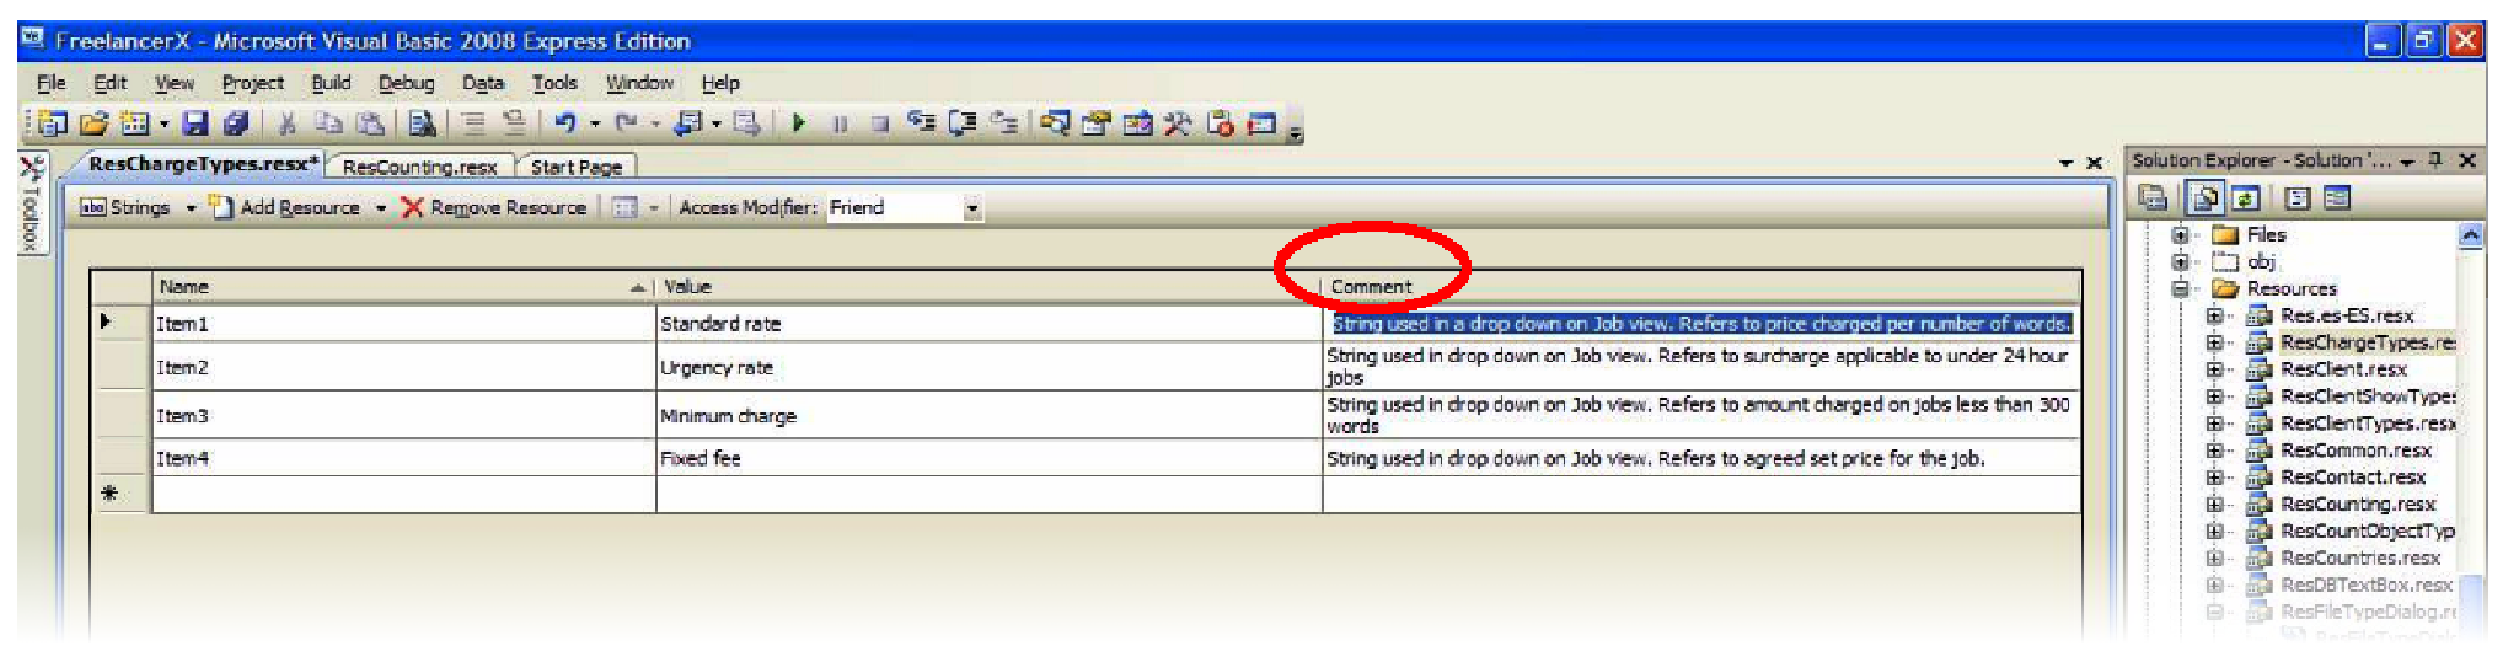
\includegraphics[width=18cm,angle=0]{images/trujamana/image1-crop.eps}

{\small\bf Figura 1. Comentario en .Net.}
\end{figure}

\clearpage
\pagebreak



\msection{introcolor}{black}{0.25}{EN LA PR�CTICA}

\begin{figure}[ht]
\centering
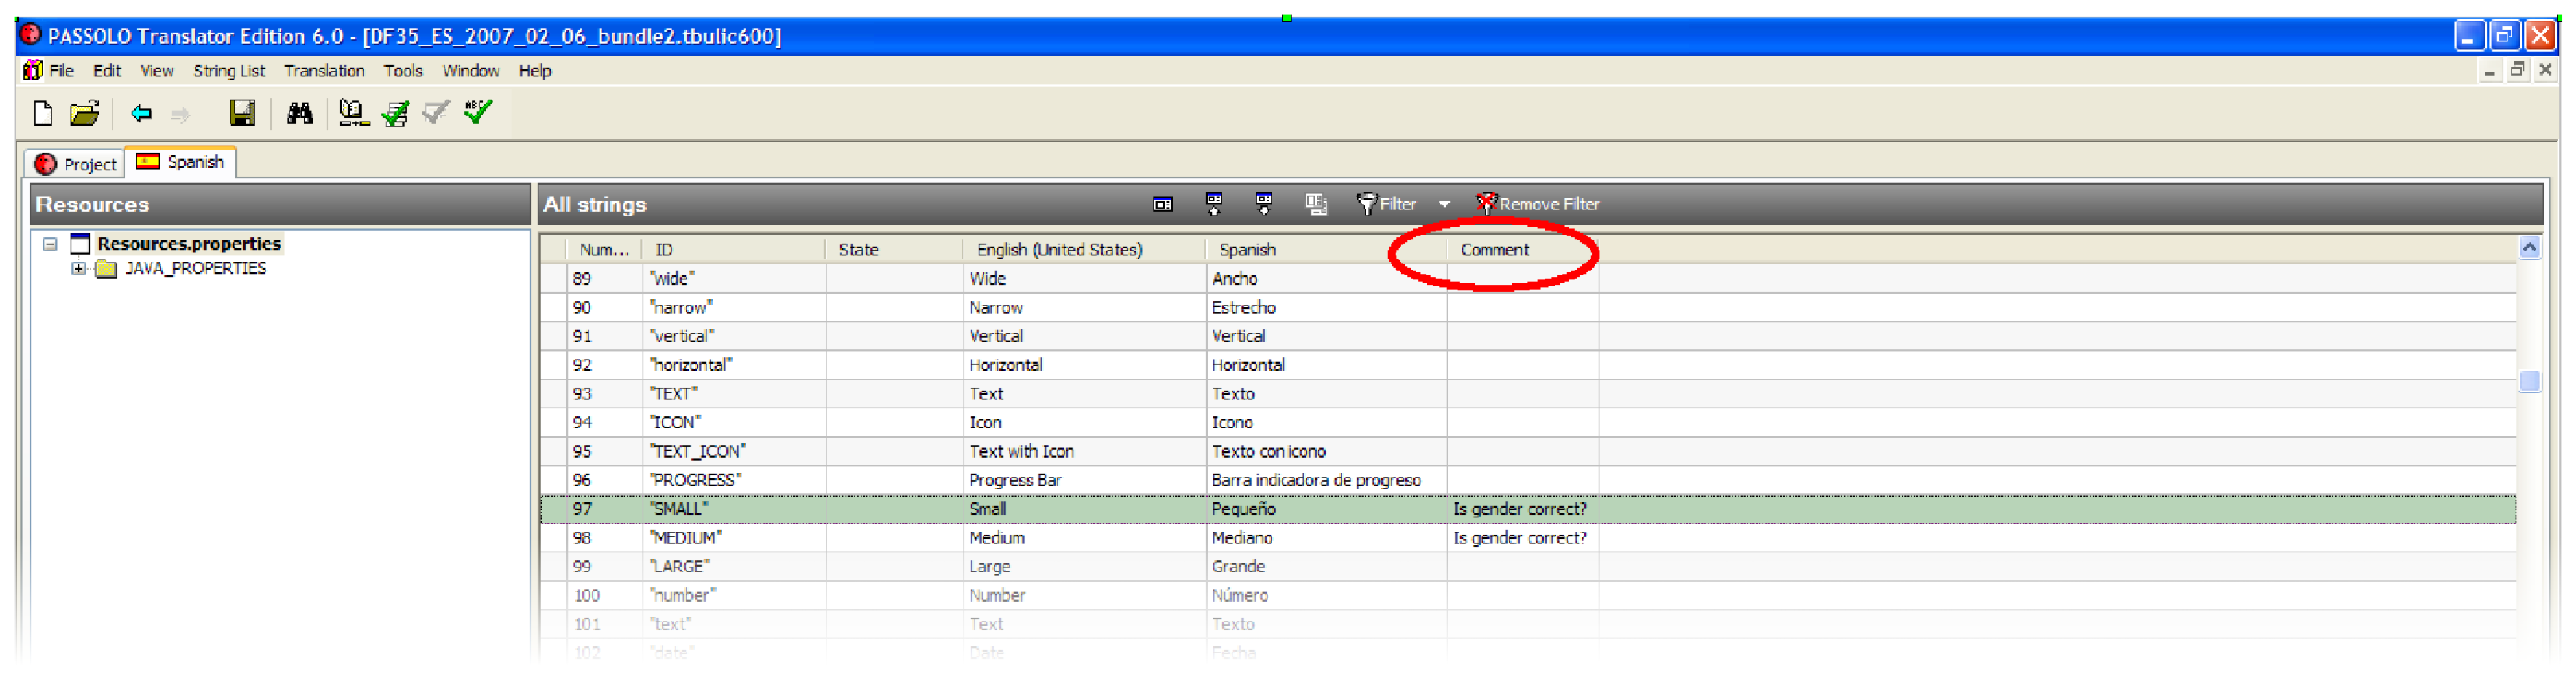
\includegraphics[width=16cm,angle=0]{images/trujamana/image2-crop.eps}

{\small{\bf Figura 2. Ejemplo de c�mo usar el campo de comentarios en Passolo \\para confirmar la traducci�n elegida.}}
\end{figure}

\begin{multicols}{2}


Como resultado en ocasiones nos encontramos ante traducciones
incorrectas y los usuarios nos sorprendemos ante el hecho de que se
haya podido traducir un t�rmino de determinada manera cuando resulta
evidente que es incorrecto. �ste es el caso del ejemplo a continuaci�n
tomado del �ltimo proyecto de localizaci�n en el que he trabajado.  

En el ejemplo que se ilustra se muestra claramente la confusi�n que
puede generar la traducci�n de una cadena sin disponer de su contexto
en la aplicaci�n. Aqu� la traducci�n del ingl�s ``languages'' se
prestaba a una traducci�n incorrecta debido a la propia naturaleza de
la aplicaci�n, una herramienta para la comparaci�n de archivos de
recursos creados en diversos lenguajes de programaci�n. 

{\scriptsize
\begin{verbatim}
IDD_OpenFileWithEncoding DIALOGEX 0, 0, 285, 33
STYLE DS_SETFONT | DS_3DLOOK | DS_FIXEDSYS | WS_CHILD | \
                   WS_VISIBLE | WS_CLIPSIBLINGS
FONT 8, "MS Shell Dlg", 0, 0, 0x0
BEGIN
  LTEXT           "&Encoding:",IDC_EncodingLabel,5,2,42,8
  COMBOBOX        IDC_Encodings,53,0,150,135,CBS_DROPDOWNLIST |\
                                      WS_VSCROLL | WS_TABSTOP 
  PUSHBUTTON      "Open from URL...",IDC_OpenUrl,211,0,62,14,\
                                     NOT WS_VISIBLE
  CONTROL         "&Languages",IDC_ShowLanguagesForEncodings, \
                  "Button",BS_AUTORADIOBUTTON | \
                  WS_GROUP,53,17,51,10
  CONTROL         "&Codepages",IDC_ShowCodepagesForEncodings, \
                  "Button",BS_AUTORADIOBUTTON,107,17,52,10
END
\end{verbatim}
}

�C�mo determinar si la traducci�n correcta en castellano debe ser ``idioma'' o ``lenguaje''? �Se refiere la cadena a un idioma humano o a un lenguaje de programaci�n?

Afortunadamente, al tratarse de una aplicaci�n peque�a que permite su instalaci�n en el ordenador del usuario, logramos resolver la diatriba simplemente buscando la instancia de esa cadena en la propia aplicaci�n.

Sin embargo, esto no siempre resulta posible ya que en ocasiones no es
factible instalar la aplicaci�n para aclarar la duda directamente,
debido a los requisitos de hardware o cuando se trata de aplicaciones
cliente servidor. En estos casos es �nicamente el programador que ha escrito esa cadena quien puede colaborar con el localizador y arrojar luz para resolver la cuesti�n. Una comunicaci�n interdepartamental fluida puede reducir considerablemente el tiempo de desarrollo de las aplicaciones adem�s de proporcionar un resultado con una calidad claramente mejorada. De lo contrario el localizador se enfrenta a un escollo insalvable y la �nica opci�n disponible es aventurarse con una traducci�n para empezar a rezar a continuaci�n. 

\end{multicols}

\begin{figure}[ht]
\centering
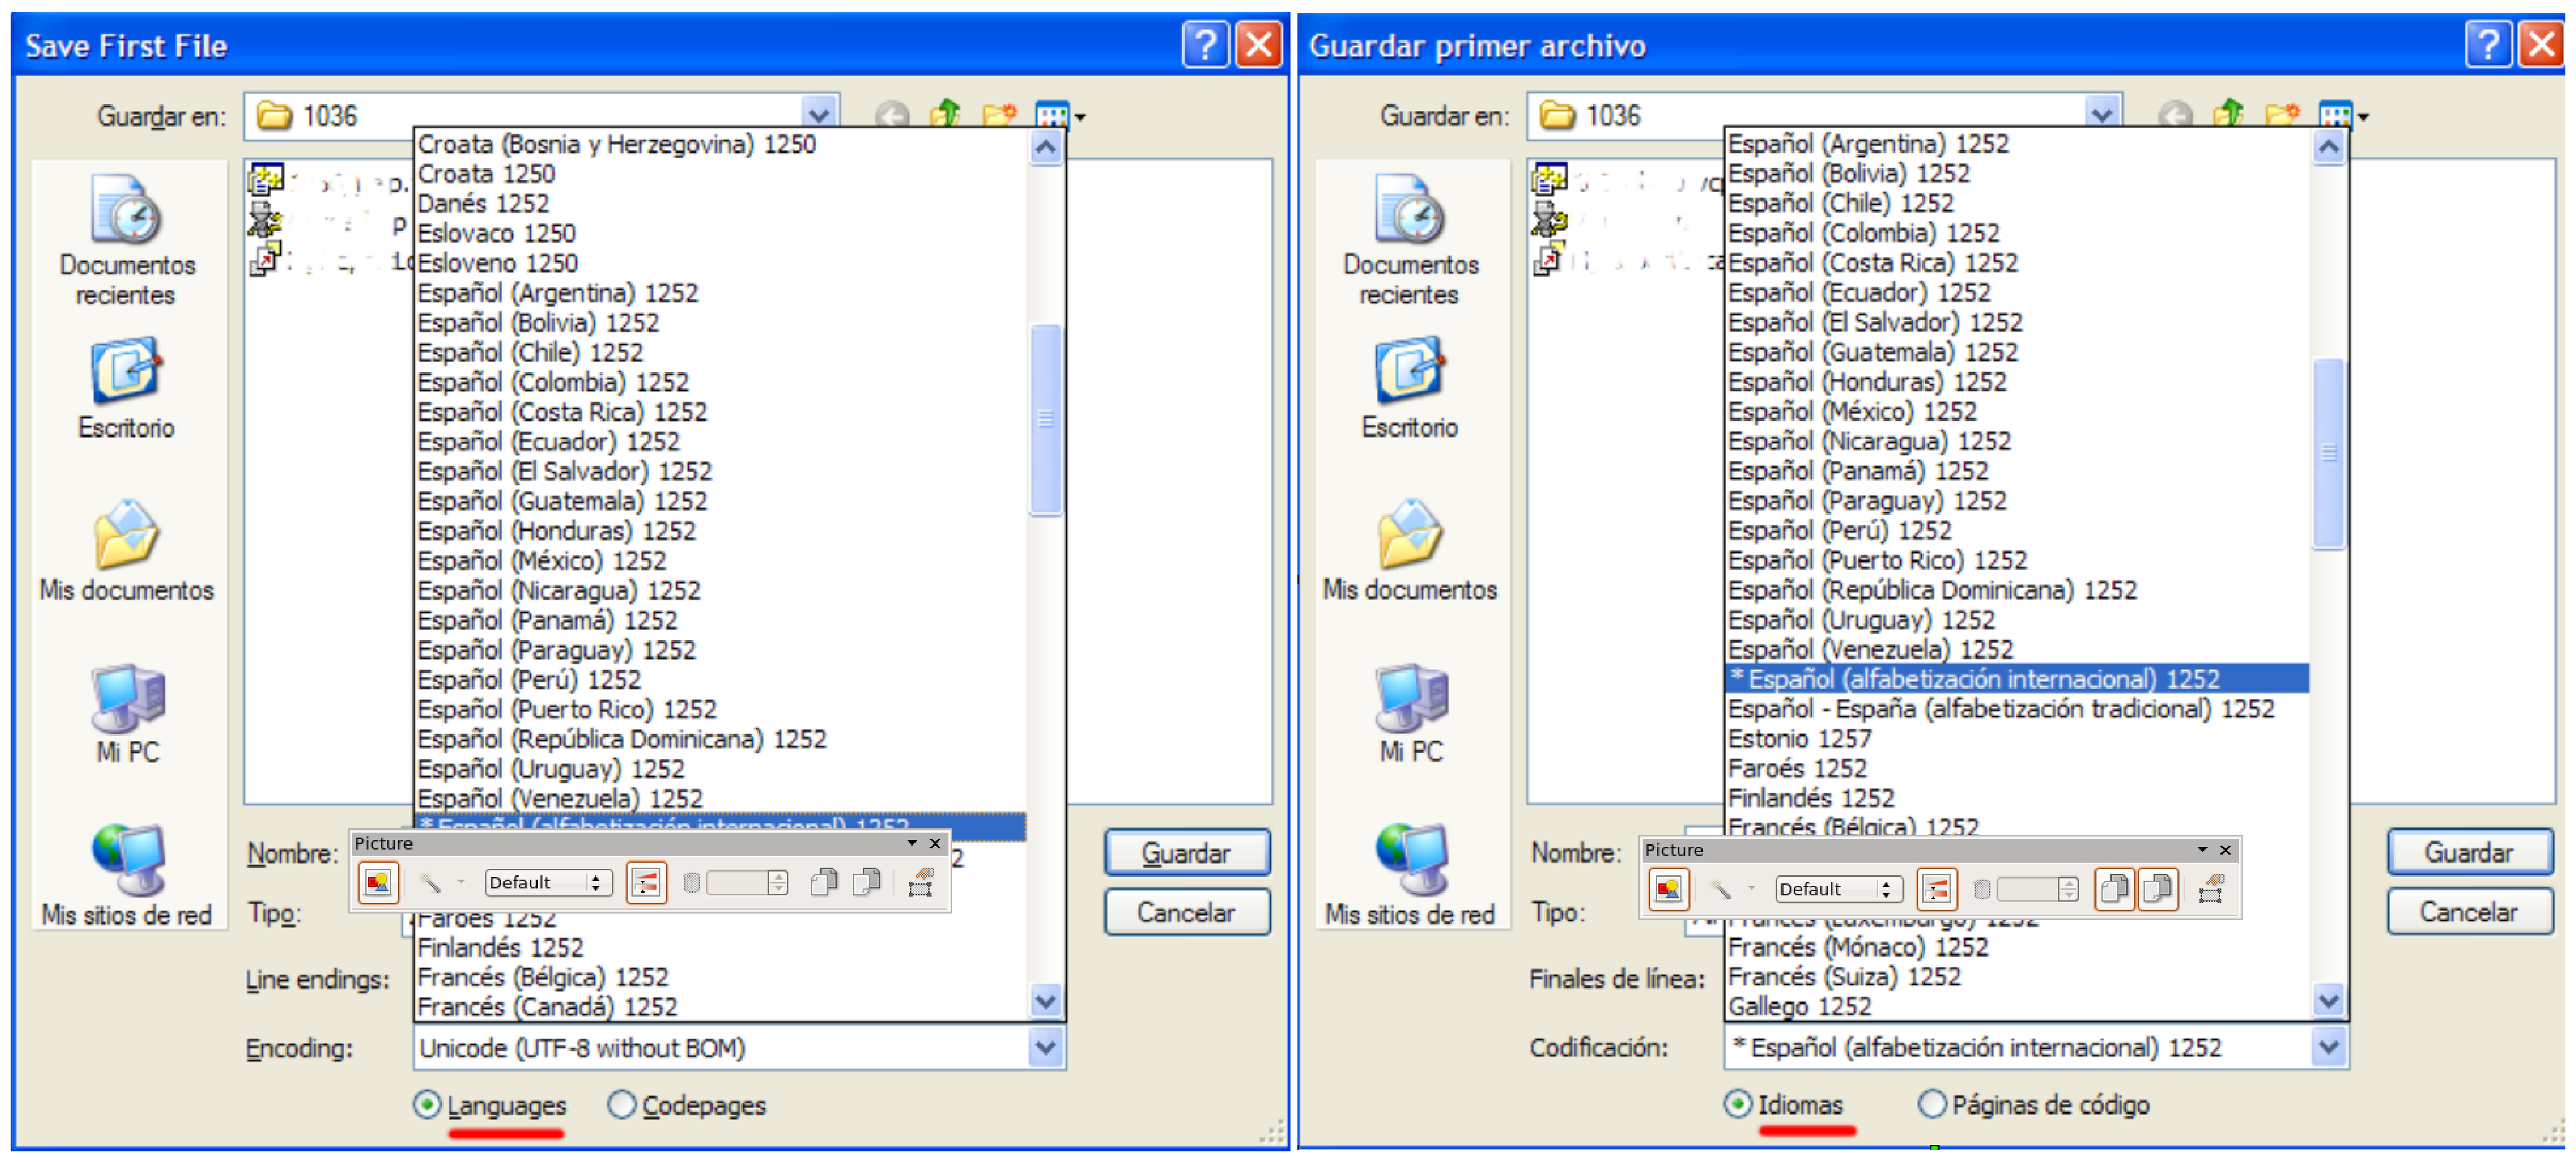
\includegraphics[width=16cm,angle=0]{images/trujamana/image3.eps}

{\small{\bf Figura 3. Ejemplo de traducci�n del t�rmino original ``languages'' en un contexto particular dentro de la aplicaci�n.}}
\end{figure}

\clearpage
\pagebreak

\bOpage{introcolor}{0.25}{EN LA PR�CTICA}

Las traducciones incorrectas debido a situaciones similares a la del ejemplo abundan. 
He aqu� un par de muestras tomadas de la localizaci�n de juegos: 

``Complete'': �C�mo traducirlo? Puede indicar que se ha superado un objetivo, un nivel o una misi�n determinada, o puede ser una instrucci�n (completar).
``All'': Seg�n a lo que se refiera ser� ``todo, todos, todas''

\begin{entradilla}
{\em La {\color{introcolor}concatenaci�n de cadenas de caracteres en
los programas} puede dificultar el proceso de localizaci�n}
\end{entradilla}

Otros ejemplos resultado de la falta de previsi�n para la
internacionalizaci�n de los productos son la concatenaci�n de cadenas
y el uso de variables. A continuaci�n se incluye una muestra de las
hojas de c�lculo utilizadas habitualmente por los localizadores para
solicitar la aclaraci�n de dudas. Estos ejemplos, est�n tomados
tambi�n de uno de mis proyectos de localizaci�n m�s recientes (ver tabla al final de esta p�gina).  

Podemos verlo a�n m�s claro en dos ejemplos ficticios tomados de Internet uno de variables y otro de concatenaci�n en la localizaci�n de videojuegos para ilustrar este concepto.

En la cadena ``John plays for \verb!{TEAM_NAME}!.'' como se puede deducir, la variable es el nombre de un equipo de f�tbol de la liga espa�ola. ``John juega en el \verb!{TEAM_NAME}!'' es una traducci�n v�lida si el equipo es el Betis, por ejemplo. Pero �y si resulta que John juega en la Real Sociedad? ``John juega en el \verb!{REAL SOCIEDAD}!''. Como siempre el problema de g�nero nos juega una mala pasada, algo que no ocurre en ingl�s al ser un idioma mucho m�s sint�tico. Como siempre con un poco de imaginaci�n y recursos se puede encontrar una soluci�n factible del tipo: ``John juega en el equipo: \verb!{TEAM_NAME}!''. 

Veamos un ejemplo de problemas de concatenaci�n en las siguientes cadenas:

\bigskip

{\small
\begin{tablehere}
\begin{tabular}{cll}
\hline
1 &	Player \%s wins a &	El jugador \%s consigue una \\
2 &	Red	& roja \\
3 &	Yellow	& amarilla \\
4 &	Green	& verde \\
5 &	Motorcycle &	moto \\
\hline
\end{tabular}
\end{tablehere}
}

\bigskip

Si no se indica al traductor que la cadena 1 va a ir unida a la cadena 2, 3 � 4 y luego a la 5, ``red, yellow, green'' podr�an traducirse en masculino o femenino. Si sabemos que estos adjetivos acompa�an a ``motorcycle'' ya sabemos que ir�n en femenino. 

Durante el juego, el jugador realiza una acci�n y es premiado con una moto verde. El programa une entonces las cadenas de la siguiente forma: 1 + 4 +5:

El resultado en ingl�s:

{\small
\begin{quote}
``Player \%s wins a green motorcycle.''
\end{quote}
}

El resultado en espa�ol:

{\small
\begin{quote}
``El jugador \%s consigue una verde moto.''
\end{quote}
}

Lo que el jugador puede interpretar como una ``mala traducci�n'' es en realidad un problema de internacionalizaci�n. 

\end{multicols}


\begin{table}[ht]
{\scriptsize
\begin{tabular}{p{2.5cm}p{1.5cm}p{3.5cm}p{4cm}p{1.3cm}p{1.9cm}}
\hline
{\bf Resource ID} & {\bf String ID} & {\bf English text}
 & {\bf Query} & {\bf ACCT Subject (Yes/No)} & {\bf Category} \\
\hline
000000067 .ProgramCurrentCostMetricsHelp.jsp & 68 & Filters for Programs or Projects where the actual costs are greater than the earned value by the specified dollar amount. & Should dollars be replaced with euros? & No & symbols \\
\hline

000000062. RequestSummaryBarChartHelp.jsp & 191 & \# of Requests & Could you confirm that '\#' means number and whether it would be okay to use the Spanish equivalent symbol �? & No &Convention \\
\hline
000000050. KPMXresourcesproperties/49 & CREATED\_ RESOLVED.TXT & created and resolved per &
Please clarify what follows after this option in order to translate correctly. & No & String not completed \\
\hline
000000033. KEXPtResourcesproperties/1574 & RED\_ EXCEPTION.TXT & of Tasks must have Exceptions to turn the Project Health & Please clarify what precedes and follows this string: i.e. is there a percentage value ``\%'' before ``of tasks''? Also, does a condition color follow ``Project Health''? & No & \\
\hline
000000012. WorkPlanResources\_en.properties/239 & warning. ActualsStartWarning warning. ActualsFinishWarning & 
\{0\} constraint \{1\} cannot be satisfied because the constraint date \{2\} is \{3\} than the Actual Start Date for the task \{4\}. The Actual Start Date takes precedence and is reflected in the Scheduled Start Date.\verb!<br><b>Resolution:</b>! If the Actual Start Date is in error, correct it and reschedule. Otherwise, changing or removing the constraint definition so that it does not conflict with the Actuals date will eliminate this warning. & 
I need to know what variables {0}, {1}, {3} and {4} will be replaced with in order to translate correctly. & No & Variables \\
\hline

\end{tabular}
}
\end{table}

\clearpage
\pagebreak

\bOpage{introcolor}{0.25}{EN LA PR�CTICA}

En ocasiones la aparici�n de una traducci�n incorrecta o fuera de
contexto se debe a situaciones como las descritas anteriormente pero, en
otras ocasiones, se deben a la automatizaci�n de los procesos de
traducci�n como es el caso del uso de las herramientas y memorias de
traducci�n. �Atenci�n a este punto! Hablamos de herramientas de
traducci�n y no de traducci�n autom�tica, dos conceptos diametralmente
diferentes.   

\sectiontext{white}{black}{TRADUCCI�N AUTOM�TICA}

El concepto de traducci�n autom�tica no requiere mayor explicaci�n ya
que es ampliamente conocido por todos. Y abundan los ejemplos de
traducciones atroces realizadas mediante todo tipo de ``artilugios''
inform�ticos, del tipo Bable Fish, etc. Ni que decir tiene que aunque
cada vez este tipo de aplicaciones est�n m�s y mejor desarrolladas,
los resultados generados no pueden equipararse a la traducci�n humana
a ning�n nivel. Aunque es cierto que en determinados contextos pueden
resultar �tiles para algunos usuarios al ayudarles a captar la idea
general de un texto, no pueden considerarse traducciones propiamente
dichas. Por eso no nos extenderemos m�s en su tratamiento. 


\sectiontext{white}{black}{HERRAMIENTAS Y MEMORIAS DE TRADUCCI�N}

Volviendo al punto de las memorias de traducci�n. �ste es, de por s�,
un tema lo suficientemente extenso como para escribir uno y muchos m�s
art�culos sobre �l. Para los no expertos en la materia: las
herramientas de traducci�n asistida (generalmente conocidos en sus
siglas en ingl�s como herramientas o aplicaciones CAT o Computer
Assisted Translation) son aplicaciones de software cuya finalidad es
la de asistir al traductor ``humano'' durante el proceso de
traducci�n; una memoria de traducci�n es b�sicamente una base de datos
usada por las herramientas CAT espec�ficas dise�adas para ayudar a los
traductores ``humanos''. Estas bases de datos contienen los segmentos
de texto en el idioma origen junto con su traducci�n a uno o varios
idiomas. Se diferencian de las bases de datos terminol�gicas en que
suelen contener bloques de texto, p�rrafos, oraciones y frases,
mientras que las otras contienen �nicamente palabras o t�rminos. 

\myfig{0}{images/trujamana/image4.eps}{1}
{\footnotesize{\bf Figura 4: Base de datos terminol�gica Multiterm 5.0}}


\myfig{0}{images/trujamana/image5.eps}{1}
{\footnotesize{\bf Figura 5: Memoria de traducci�n Trados Workbench
 6.5 con los segmentos guardados.  }}

\bigskip

Las herramientas CAT y las memorias de traducci�n representan una
ayuda valios�sima a la tarea del traductor o localizador, ya que
permiten reutilizar los segmentos coincidentes que hayan sido
traducidos previamente. Ello supone un considerable ahorro de tiempo
adem�s de contribuir a mantener la consistencia en la traducci�n de
los t�rminos m�s habituales espec�ficos de un determinado proyecto.  

\begin{entradilla}
{\em Las {\color{introcolor} memorias de traducci�n son una herramienta} imprescidible}
\end{entradilla}

El proceso es simple. A grandes rasgos y generalizando un poco, ya que
cada herramienta presenta peculiaridades espec�ficas en su
funcionamiento, se puede decir que funcionan del siguiente modo. El
traductor abre el documento que va a traducir en la herramienta CAT
(algunas usan su propia interfaz mientras que otras se integran e
interact�an con procesadores de texto del tipo MS Word) y procede a
escribir la traducci�n para cada segmento que aqu�lla abre. Cada vez
que se cierra o se guarda un segmento, la herramienta de traducci�n
almacena el texto en el idioma original con su traducci�n
correspondiente en la memoria. A medida que se avanza en la
traducci�n, la herramienta CAT junto con la memoria de traducci�n
mostrar� al traductor los segmentos coincidentes que se hayan
traducido anteriormente, bien en un 100\% de concordancia o en
porcentajes inferiores, para reutilizarlos. Asimismo, permiten
realizar b�squedas espec�ficas de t�rminos frecuentes entre todos los
segmentos traducidos almacenados en la memoria. La herramienta de
traducci�n define cada segmento que se traduce de acuerdo con las
definiciones proporcionadas por el usuario. La gran mayor�a de ellas
usan los signos ortogr�ficos como marcadores de segmentos, es decir,
puntos, puntos y comas, etc. 



\end{multicols}
\clearpage
\pagebreak


\msection{introcolor}{black}{0.25}{EN LA PR�CTICA}

\vspace{1cm}

\begin{figure}[ht]
\centering
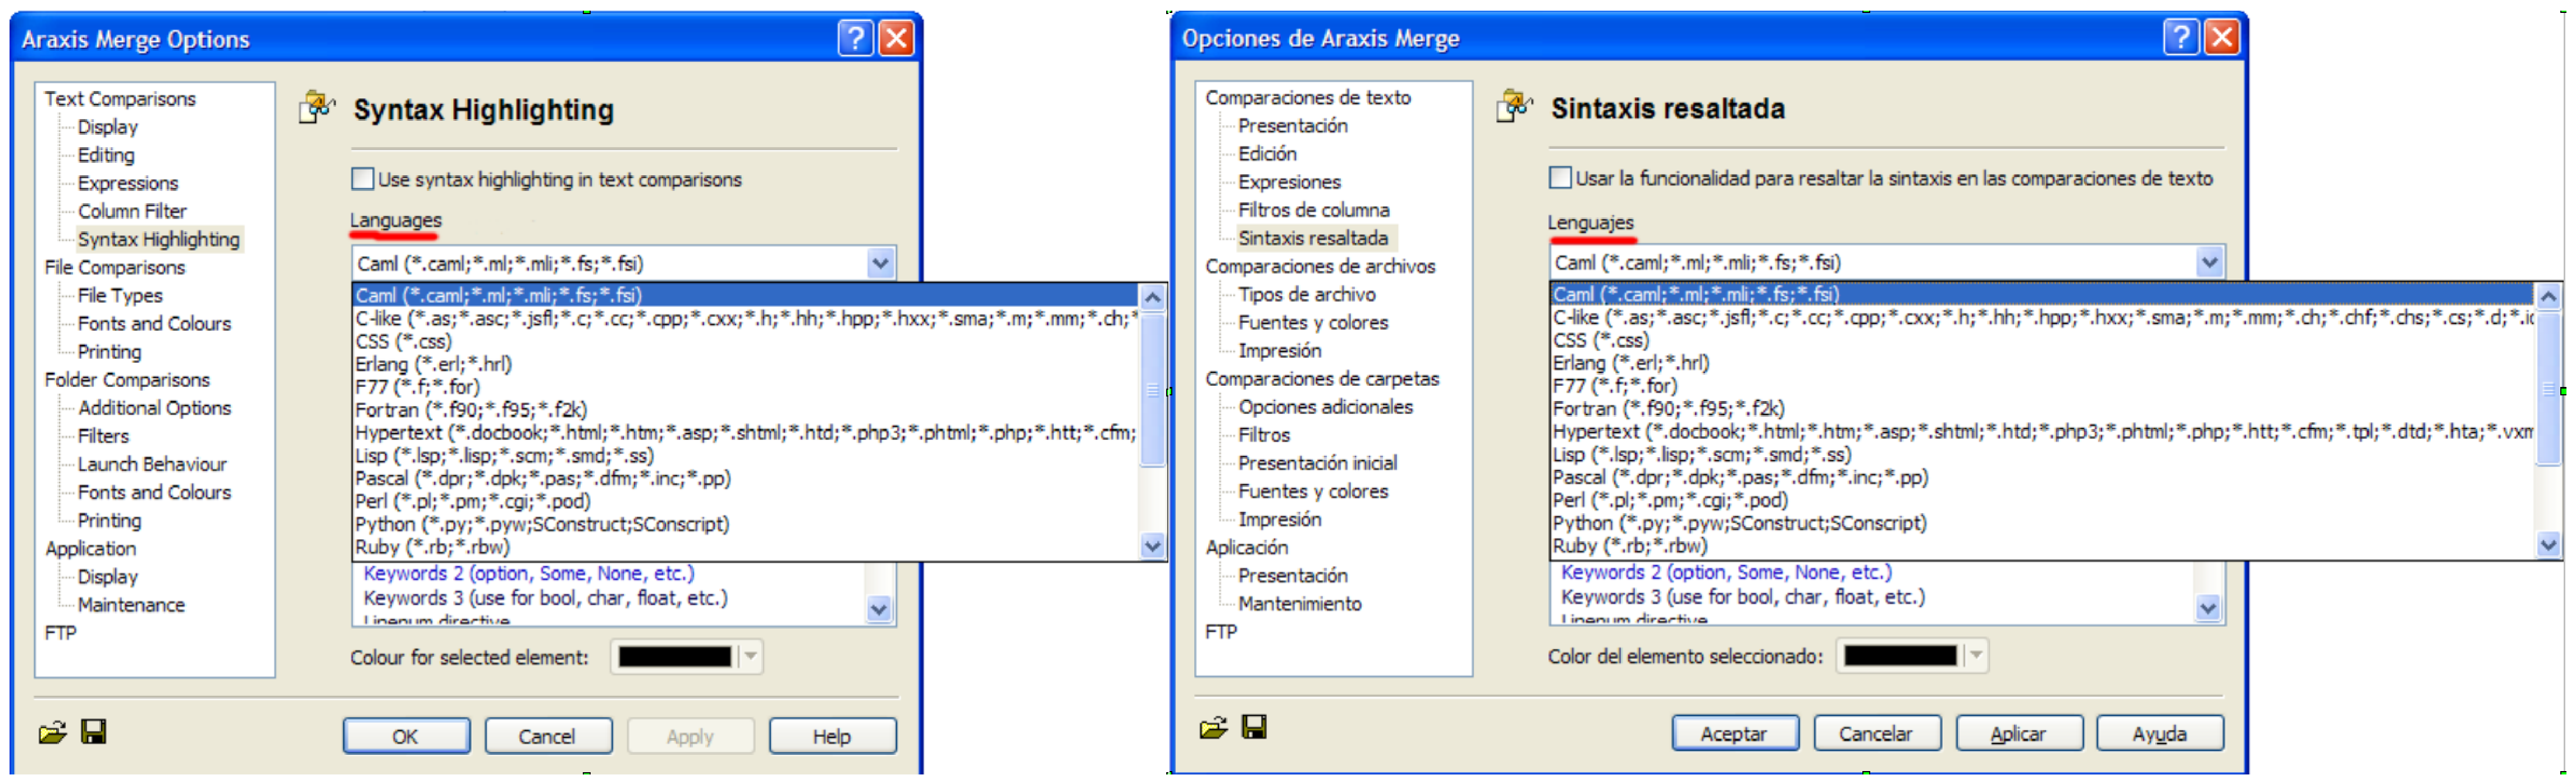
\includegraphics[width=17cm,angle=0]{images/trujamana/image6.eps}

{\small{\bf Figura 6. Ejemplo de traducci�n del t�rmino original ``languages'' en otro contexto diferente dentro de la misma aplicaci�n. }}
\end{figure}


\begin{multicols}{2}



Algunas de estas herramientas tambi�n ofrecen la posibilidad de
procesar el documento para realizar una pretraducci�n usando los
segmentos almacenados en la memoria de traducci�n. Esta pretraducci�n
podr� hacerse tambi�n de acuerdo con los criterios de concordancia
establecidos. As� podr�n usarse concordancias del 100\% o en franjas
de porcentajes inferiores.  

Muchas tambi�n ofrecen la posibilidad de trabajar individualmente o
conectados en red compartiendo los contenidos almacenados en las
memorias entre varios traductores. 

Como puede verse, las memorias de traducci�n suponen un excelente
reaprovechamiento de recursos y garantizan un mayor grado de
coherencia interna de la terminolog�a. No obstante, no est�n exentas
de riesgo. En relaci�n a lo que dec�amos anteriormente, una misma
cadena puede ser utilizada en un contexto diferente con un significado
totalmente distinto, tal como se ilustra en la Figura 6. Es evidente que la traducci�n del t�rmino ``languages''
aqu� no podr�a ser nunca la misma que la que se mostraba en uno de los
ejemplos anteriores, aunque ambos est�n extra�dos de la misma
aplicaci�n. 



Esto resulta particularmente relevante cuando, por ejemplo, varios
traductores est�n trabajando compartiendo en red una misma memoria
global de traducci�n para un mismo cliente. Mientras que unos est�n
realizando la traducci�n de las cadenas de software, otros est�n
trabajando en los materiales colaterales (manuales de usuario,
manuales t�cnicos, marketing, etiquetado y empaquetado, intranet,
etc.). Incluso en estos casos aunque existan concordancias del 100\%,
la traducci�n no tiene por qu� ser necesariamente igual. 

\begin{entradilla}
{\em Las memorias de traducci�n facilitan {\color{introcolor}la coherencia interna de la
terminolog�a} }
\end{entradilla}

Lo que es
m�s, probablemente no deber�an ser iguales puesto que, por ejemplo,
las terminaciones de los verbos en -ing del ingl�s podr�n traducirse
como un infinitivo en las cadenas de c�digo de la aplicaci�n pero como
un sustantivo o incluso como una frase f�rmula del tipo ``C�mo...'' en
manuales de usuario o materiales de marketing. 

\begin{entradilla}
{\em Una misma cadena puede ser utilizada en {\color{introcolor}un contexto 
diferente con un significado} totalmente diferente}
\end{entradilla}

Otros ejemplos de diferentes usos dependiendo del �mbito de uso:  

\bigskip

\begin{tablehere}
{\scriptsize
\begin{tabular}{|p{2cm}p{2.5cm}p{2.5cm}|}
\hline
Texto Origen & Traducci�n para Documentaci�n & Traducci�n para Software \\
\hline
Printing a range and a Graph &
Impresi�n de un intervalo y de un gr�fico o C�mo imprimir un intervalo
y un gr�fico &
Imprimir un intervalo y un gr�fico \\
\hline
Delete Links & Supresi�n de enlaces o C�mo... & Suprimir enlaces \\
\hline
Apply symbols & Aplicaci�n de los s�mbolos o C�mo... & Aplicar
s�mbolos \\

\hline
\end{tabular}
}
\end{tablehere}

\bigskip

Por ello, es esencial disponer de los medios (bien sea mediante la
instalaci�n de la aplicaci�n o la colaboraci�n con los programadores
responsables o el personal de marketing) para garantizar que una
cadena de texto determinada es apropiada en el contexto en el que va a
aparecer.  

Este aspecto es de particular relevancia ya que durante la fase de
testing o de control de calidad existe un probabilidad muy alta
de que pase desapercibido puesto que este tipo de tareas, por lo
general, suelen estar desempe�adas por testers que no hablan el idioma
o idiomas a los que se ha traducido la aplicaci�n.  


\eOpage

\rput(9.0,-23.7){\resizebox{!}{7.2cm}{{\epsfbox{images/trujamana/image8.eps}}}}

\bOpage{introcolor}{0.25}{EN LA PR�CTICA}

\sectiontext{white}{black}{EMPRESAS L�DERES DEL MERCADO}

Evidentemente, dependiendo de la herramienta utilizada, la facilidad o
dificultad para identificar y procesar estas cadenas variar� de forma
considerable. En la actualidad, podr�a decirse que el l�der del
mercado para la traducci�n general as� como para la localizaci�n de
software comercial es SDL Trados, seguido de Transit y DejaVu. En un
�mbito m�s t�cnico se encontrar�an Catalyst y Passolo. Como nota de
inter�s, la mayor�a de estas aplicaciones son desarrolladas por
empresas alemanas.  

\begin{tablehere}
{\scriptsize
\begin{tabular}{|p{2.0cm}|p{1.1cm}p{0.9cm}p{0.9cm}p{0.9cm}|}
\hline
   & Atril  Deja-Vu X & TRADOS 7 & STAR Transit XV & SDL  Translation Suite 2006 \\
\hline
Ayuda al traductor & & & &  \\
\hline
Revisor ortogr�fico  & S� & S� & S� & S� \\
Tesauro & S� & S� & No & No \\
Glosario & S� & S�  & S� &  S� \\
BD terminol�gica & S� & S� & S� & S� \\
Diccionarios & S� & S� & S� & S� \\
Interfaz de traducci�n propia & S� & S� & S� & S� \\
Alineaci�n  & S�  & S� & S� & S� \\
Extracci�n de t�rminos  & No & S� & No & No \\
Interfaz de TA & No & No & S� & S� \\
\hline
Tipos de archivo & & & & \\
\hline
DLL, EXE & No & S� & No & No \\
Excel & S� & S� & S� & S� \\
PowerPoint & S� & S� & S� & S� \\
RC & S� & S� & S� & S� \\
RTF (Win Help) & S�  & S� & S� & S� \\
RTF (Texto) & S� & S� & S� & S� \\
TXT & S� & No & S� & S� \\
DOC & S� & S� & S� & S� \\
Framemaker & S� & S� & S� & S� \\
PageMaker & No & S� & S� & S� \\
HTML & S� & S� & S� & S� \\
\hline
Reutilizaci�n & & & & \\
\hline
Coincidencias parciales & S� & S� & S� & S� \\
Coincidencias id�nticas & S� & S� & S� & S� \\
De mismo tipo de objeto & S� & No & No & No \\
Basado en frases & S� & S� & S� & S� \\
Basado en p�rrafos & S� & S� & S� & S� \\

\hline
\end{tabular}
}
\end{tablehere}

{\footnotesize\bf Fuente: www.traductores.org.ar}

\bigskip
\columnbreak

Por supuesto, en el �mbito de software libre tambi�n existen
aplicaciones equivalentes como, por ejemplo, OmegaT. As� mismo y
aunque no encuadradas bajo el grupo de herramientas CAT tambi�n
existen bibliotecas de software del tipo de gettext que facilitan la
tarea de localizaci�n de aplicaciones. 



\sectiontext{white}{black}{RETOS DEL LOCALIZADOR}

La labor del localizador de software es silenciosa pero omnipresente
en la actualidad. En su trabajo diario se enfrenta a numerosos retos y
dificultades inherentes a la naturaleza de este trabajo. Puesto que el
lenguaje evoluciona a una velocidad vertiginosa particularmente en el
�mbito de la inform�tica mediante la introducci�n de neologismos, el
traductor/localizador debe tener una clara conciencia de su labor como
ling�ista adem�s de como experto en otros aspectos m�s especializados
del proceso de localizaci�n. Por ello, para ser un buen localizador no
basta con ser un buen traductor. Adem�s de ser un maestro del lenguaje
tambi�n hay que poseer excelentes aptitudes t�cnicas y un gran
entusiasmo, porque localizaci�n es el arte de la traducci�n convertido
en ciencia.   



Y eso es algo que el localizador debe aprender mediante una s�lida
formaci�n acad�mica y amplia experiencia en el �mbito laboral, ya que
no es algo que necesariamente venga predeterminado (del ingl�s {\em by
default} que no por defecto!!...)

\begin{center}
\colorbox{excolor}{
\begin{minipage}{.98\linewidth}
{\bf\sf\Large Sobre la Autora}
\vspace{1mm}
\hrule
\bigskip
\small

Silvia Carril Caldelas es licenciada en Traducci�n e Interpretaci�n por la
Universidad de Vigo. Desde 1997 trabaja como especialista en localizaci�n de
software para empresas tanto del Reino Unido como de Espa�a. Actualmente es
la directora de ilia, compa��a brit�nica especializada en la localizaci�n y
desarrollo de software. 

{\tt silvia@ilialang.com // www.ilialang.com}

\bigskip

\end{minipage}
}
\end{center}

\normalsize
\raggedcolumns



\end{multicols}
\begin{center}
Fig. 8: Volcado de pantalla de Catalyst 7.0
\end{center}

\clearpage
\pagebreak


% Este fichero es parte del N�mero 3 de la Revista Occam's Razor
% Revista Occam's Razor N�mero 3
%
% (c)  2007, 2008, 2009, The Occam's Razor Team
%
% Esta obra est� bajo una licencia Reconocimiento 3.0 Espa�a de
% Creative Commons. Para ver una copia de esta licencia, visite
% http://creativecommons.org/licenses/by/3.0/es/ o envie una carta a
% Creative Commons, 171 Second Street, Suite 300, San Francisco,
% California 94105, USA. 

% Seccion Ratas de Tutorial
%
% Incluye imagen del art�culo


\rput(3,-2.1){\resizebox{!}{2.8cm}{{\epsfbox{images/odeon/odeon.eps}}}}

% -------------------------------------------------
% Cabecera
\begin{flushright}
\msection{introcolor}{black}{0.25}{TUTORIAL}

\mtitle{10cm}{Introducci�n a la Simulaci�n Ac�stica}

\msubtitle{8cm}{Aprendemos a utilizar ODEON}

{\sf por Francisco Miguel Bellas Al�ez}

{\psset{linecolor=black,linestyle=dotted}\psline(-12,0)}
\end{flushright}

\vspace{2mm}
% -------------------------------------------------

\begin{multicols}{2}


% Introducci�n
\intro{introcolor}{C}{uando se oye hablar de realidad virtual uno
  siempre piensa en mundo 3D creados mediante programas de
  renderizado. Sin embargo, tambi�n existe la virtualizaci�n sonora,
  es decir, crear entornos virtuales que transformen un sonido de una
  forma determinada. En este art�culo voy a presentar uno de estos
  programas y, al mismo tiempo, voy a ir dando unas nociones b�sicas
  sobre an�lisis y dise�o ac�stico de salas.  
}

\vspace{2mm}

% Cuerpo del art�culo

Podremos medir y comprobar mediante n�meros y gr�ficas si una sala
responde como nosotros queremos pero tambi�n podremos probar dicha
sala escuchando un sonido, una conversaci�n o una melod�a como si
estuvi�ramos en dicha sala. 

Usaremos a lo largo del art�culo  el programa de an�lisis ac�stico
Odeon que, aunque no es gratuito, si dispone de una versi�n
demostraci�n que permite trabajar con algunas salas predefinidas, lo
cual servir� para asimilar los conceptos b�sicos del dise�o y an�lisis
de salas. Esta gu�a est� basada en las pr�cticas de uno de los
laboratorios de ac�stica de la ETSIT de Vigo. 

\sectiontext{white}{black}{INSTALACI�N DE ODEON}

Odeon es un programa de simulaci�n ac�stica de salas que nos ayuda
tanto al dise�o de nuevas salas como al an�lisis ac�stico de salas ya
construidas. En su versi�n completa, este programa permite crear salas
en 3D incluyendo los materiales de que est� compuesta para luego
someter dicha sala a una serie de algoritmos de simulaci�n ac�stica
que nos permiten medir los principales par�metros de calidad ac�stica
de salas. En este art�culo trabajar� con la versi�n limitada
(demostraci�n) que permite s�lo trabajar con las salas predefinidas. 

\begin{entradilla}
{\em Odeon ha sido creado por el {\color{introcolor}Departamento de Tecnolog�a Ac�stica}
  de la Universidad T�cnica de Dinamarca}
\end{entradilla}

Odeon ha sido creado por el Departamento de Tecnolog�a Ac�stica de la
Universidad T�cnica de Dinamarca y puede ser descargado de la web: 

{\small
\begin{verbatim}
http://www.odeon.dk/
\end{verbatim}
}

en el apartado downloads. En el momento de escribir este art�culo
dicha p�gina ofrece la versi�n 9.0 del programa. Os lo pod�is bajar en
un �nico fichero zip para Windows. Si ten�is Linux pod�is probar a
instalar en alguna m�quina virtual tipo VirtualBox. Parece que se
puede ejecutar directamente sobre wine, aunque no hemos probado todas
sus funcionalidades.

La instalaci�n es realmente simple. Desomprim�s el zip en una carpeta
y ejecut�is el programa setup.exe. Pr�cticamente la �nica opci�n que
hay que seleccionar es vuestra carpeta destino que, curiosamente y al
rev�s que en otros programas, no se instala en  

{\small
\begin{verbatim}
C:\Archivos de programa\
\end{verbatim}
}

si no directamente en el ra�z del disco duro fuente. Cambiadlo a
vuestro gusto y punto. 

\bigskip

\colorbox{excolor}{
\begin{minipage}{1\linewidth}
\sf
\begin{center}
{\color{black}{\textbf {PAR�METROS AC�STICOS DE INTER�S}}}
\end{center}

\medskip

Existen diversas teor�as ac�sticas que ayudan a obtener distintos
par�metros de calidad de una sala. La teor�a estad�stica permite
mediante modelado probabil�stico del campo ac�stico obtener la energ�a
ac�stica en distintas partes de una sala y, por tanto, nos permite
obtener niveles de reverberaci�n. La teor�a geom�trica modela la
propagaci�n sonora mediante el trazado de rayos de forma similar a
como se trabaja en �ptica. Finalmente la teor�a ondulatoria obtiene la
ecuaci�n de onda en la sala y obtiene la respuesta en frecuencia de la
misma. Veamos algunos de los par�metros principales que manejan estas
teor�as: 

\begin{itemize}

\item {\bf Coeficiente de absorci�n:} Relaci�n entre la energ�a incidente y
reflejada en una superficie. 

\item {\bf Tiempo de Reverberaci�n (TR):} Se define como el tiempo en que tarda la
energ�a ac�stica en atenuarse 60 dB una vez que cesa la emisi�n de la
fuente (la millon�sima parte en unidades naturales). Si en un recinto
los materiales son ac�sticamente muy reflectantes este tiempo ser�
mayor (se percibir� efecto de un eco muy corto) y si son absorbentes
ser� menor. Dependiendo del destino de la sala, un TR muy bajo puede
ser bueno para que se entienda mejor a un orador, pero puede darle
mucha ``frialdad'' a una sinfon�a. 

\item {\bf �rea de absorci�n equivalente:} Ponderaci�n entre las diversas
superficies que tiene una sala seg�n su absorci�n y establecer un
equivalente mediante una �nica superficie de determinada �rea que
tenga la misma absorci�n. 

\medskip

\end{itemize}
\end{minipage}
}

\ebOpage{introcolor}{0.25}{TUTORIAL}

\sectiontext{white}{black}{COMENZANDO CON ODEON}

A continuaci�n vamos a familiarizarnos con el programa Odeon para
realizar luego una serie de ejemplos guiados en los cuales quedar� m�s
claro los conceptos explicados previamente. Tras abrir el entorno de
trabajo nos encontramos con un formulario con sus men�s, iconos y un
fondo de pantalla absolutamente horrible y que puede parpadear de
forma muy inc�moda dependiendo de la frecuencia de refresco de nuestro
monitor.  

\myfig{0}{images/odeon/image1.eps}{1}
\begin{center}{\footnotesize{\bf Figura 1. 3D View}}\end{center}
\medskip



Abramos a continuaci�n una de las salas que vienen predefinidas
(recordemos que en la versi�n demo s�lo se puede trabajar con estas
salas) entrando en el men� File->Open Room. Escogemos por ejemplo la
sala auditorium 21 (los archivos son los de extensi�n .par).  Se abre
una ventana denominada 3D View en la que  aparece el modelo 3D de
dicha sala que podemos girar y colocar a nuestro aire mediante el
rat�n. Tambi�n pulsando la barra espaciadora podemos cambiar ciertas
vistas predeterminadas (planta, alzado, etc.) 


Aparece tambi�n un nuevo men�, el 3D View que permite realizar
distintas tareas con la ventana de representaci�n 3D: Podemos ampliar
o reducir con la opci�n zoom; mediante Highligh Surfaces se nos
muestra una lista de superficies en la parte inferior. Pulsando en
alguna de ellas la resalta en el dibujo; mediante Show Corner numbers
and coor se pueden ver las coordenadas de las esquinas de la
superficie seleccionada y se resalta la esquina seleccionada con un
c�rculo azul. 


\begin{entradilla}
{\em La {\color{introcolor}ventana 3D View} nos muestra nuestra sala en 3D}
\end{entradilla}


Os recomiendo jugar con las distintas opciones de este men� que
afectan exclusivamente a la visualizaci�n de la sala. Tambi�n os
recomiendo abrir distintas salas y ver las caracter�sticas de las
mismas.  

En el men� Toolbar hay algunas opciones m�s que son interesantes como
primera toma de contacto. Una de ellas es Room Information que nos da
datos sobre las dimensiones de la habitaci�n. Otra es la vista 3D
OpenGL que nos permite echar un vistazo a la sala como si estuvi�ramos
dentro de ella. Tambi�n es interesante la opci�n 3D Reflector Coverage
que nos muestra mediante c�digo de colores que zonas de la sala son
reforzadas por los reflectores para distintas fuentes (sources). Hay
m�s opciones pero que introduciremos en sucesivos apartados ya que es
preferible verlas definiendo nosotros los par�metros que podamos y no
limit�ndonos a visualizar algo ya hecho. De todas formas pod�is probar
la 3D Billiard o la 3D Investigate Rays que son simulaciones bastante
espectaculares de la evoluci�n de una onda o de rayos sonoros. 

Finalmente quedaros con la sala Example ya que es muy sencilla y para
aprender el manejo de Odeon y los conceptos de ac�stica es la m�s
clara. Luego experimentaremos con alguna sala m�s compleja. 

\sectiontext{white}{black}{DEFINICI�N DE MATERIALES USADOS}

Aunque la versi�n demo de Odeon no deje modificar la sala, s� permite
cambiar los materiales de la misma para hacer distintas pruebas. 

Si ten�is abierta la sala Example, pod�is pinchar la opci�n del men�
Toolbar->Material List y se abrir�n dos ventanas. En la superior
aparece la representaci�n de la sala y en la inferior la lista de
superficies a la izquierda y la librer�a de materiales disponibles en
el programa a la derecha.  

\begin{entradilla}
{\em Podremos {\color{introcolor}modidicar los materiales} de nuestra sala}
\end{entradilla}

Pinchando sobre cualquier material de la lista de la derecha, aparece
en la parte inferior su repuesta en frecuencia (en referencia al
coeficiente de absorci�n) en las bandas de octava 63, 125, 250, 500,
1000, 2000, 4000 y 8000 Hz que son est�ndar en medidas
ac�sticas. 

\myfig{0}{images/odeon/image2.eps}{1}
\begin{center}{\footnotesize{\bf Figura 2. Lista de Materiales}}\end{center}
\medskip

\ebOpage{introcolor}{0.25}{TUTORIAL}

Tambi�n mediante un gr�fico de barras peque�o a la
izquierda se puede intuir de forma visual la respuesta en frecuencia
del material.  




Los primeros materiales de la lista son ideales. Es decir, son
materiales con un porcentaje de absorci�n determinado en todas las
frecuencias. Los materiales reales aparecen a partir del 99. 


La parte interesante de esto es la posibilidad de asignarle los
materiales que nos apetezca a las distintas superficies de la
sala. Para ello lo primero que se hace es seleccionar el material en
un lado y la superficie en el otro. Luego se pulsa en el icono de
Asignaci�n de Material que es el primero que aparece en la columna que
separa la lista de materiales de la lista de superficies (en la misma
ventana Material List) 

\myfig{0}{images/odeon/image3.eps}{0.1}
\begin{center}{\footnotesize{\bf Figura 3. Icono de Asignaci�n de Materiales}}\end{center}
\medskip


Por ejemplo podemos tomar la superficie 1001 que es donde estar�a la
orquesta y asignarle el material 900 que es un material que simula la
absorci�n de una orquesta con instrumentos. Luego seleccionamos la
1002, que es la audiencia y le podemos asignar uno de los valores
entre el 903 y el 909 que son distintos tipos de zonas audiencia con
sillas de distintos materiales. Por ejemplo el 903. Al resto de las
superficies (techos y paredes) le podemos asignar un material poco
absorbente como el 700. 

El par�metro scatter indica la difusi�n en la reflexi�n del
sonido. Poned todos a 0,1 salvo los materiales 1001, 1002 y 2004 que
les pod�is aumentar la difusi�n a 0,7. 

\sectiontext{white}{black}{FUENTES Y RECEPTORES}

Una vez que tenemos definida la sala, para realizar alg�n tipo de
simulaci�n es necesario especificar d�nde colocamos las fuentes
sonoras y d�nde se desea colocar el receptor o los receptores. 

 Seleccionamos del men� Toolbar la opci�n Source Receiver List. Se nos
 abre una ventana donde podemos especificar fuentes (sources) y
 receptores (receivers). Pulsando la letra P o en el icono New Point
 Source (similar a una diana roja) a�adimos fuentes y pulsando R o
 sobre el icono del micr�fono (New Receiver) a�adimos receptores. 

\medskip

{\small
\begin{tablehere}
\begin{tabular}{cp{.7\linewidth}}
\hline

\includegraphics[width=0.7cm]{images/odeon/image3-1.eps} & New Point Source\\

\includegraphics[width=0.7cm]{images/odeon/image3-2.eps} & New Receiver \\

\hline
\end{tabular}
\end{tablehere}
}

\medskip

Pulsamos primero la P y se nos abre una ventana donde podemos
introducir diversos par�metros. La descripci�n es el nombre que le
queramos dar a la fuente. En las coordenadas colocaremos  

\bigskip

$x=3$	$ y=0$	 $z=1,7 $

(usa la coma para los decimales)

\bigskip

A medida que modificamos las coordenadas podemos ver la fuente como un
c�rculo rosa en la ventana 3DView.  Mediante Azimut, elevaci�n y
rotaci�n podemos indicar hacia d�nde apunta la fuente. En principio
podemos dejarlo a cero (En 3DView viene indicado por una l�nea que
sale del c�rculo). 

En la parte inferior indicamos una ganancia (Overall gain) de 65 dB
que es la potencia de emisi�n. El apartado EQ es por si se desea
ecualizar la fuente para darle cierta ``forma en frecuencia''.  

Cerramos la ventana. S�, en el icono X de la propia ventana. No hay
bot�n aceptar as� que no lo busqu�is ;). Nos aparece la fuente creada
en la lista.  

Para definir receptores pulsamos la tecla R. Aparece una ventana
similar pero m�s sencilla. S�lo se indica coordenada. Aparece tambi�n
un icono de Open GL ya que una vez colocado el receptor podr�amos
comprobar la vista que tiene de la sala desde la posici�n indicada. 

Crear dos receptores, uno en $x=8, y=-5, z=1,5$ y el otro en $x=20, y=2, z=4$.

\sectiontext{white}{black}{C�LCULOS DE TIEMPO DE REVERBERACI�N}

Lo primero que haremos ser� hacer una estimaci�n del tiempo de
reverberaci�n mediante teor�a estad�stica. Para ello ten�is que abrir
primero la Material list y luego seleccionar la opci�n Quick Estimate
en el men� Materials. 

Nos aparece un gr�fico (pesta�a Estimations) que nos muestra el tiempo
de reverberaci�n de la sala (RT) en segundos para distintas
frecuencias seg�n 3 m�todos distintos: ecuaci�n de Eyring, de Sabine y
de Arau-Puchades.  Estos m�todos cambian en cuanto a precisi�n y
complejidad de c�lculo. 

\myfig{0}{images/odeon/image4.eps}{1}


En la pesta�a Material Overview podemos ver la absorci�n de cada uno
de los materiales seg�n la frecuencia. 

\ebOpage{introcolor}{0.25}{TUTORIAL}

Esto es muy �til ya que nos puede ayudar a ajustar los materiales de la sala si notamos que hay excesiva absorci�n o demasiada reflexi�n para algunas frecuencias. Cabe destacar tambi�n que el aire realmente afecta mucho en altas frecuencias y las aten�a por absorci�n. La p�rdida de altas frecuencias provoca una p�rdida en el ``brillo'' de la m�sica.

\myfig{0}{images/odeon/image5.eps}{1}
\bigskip

Podemos ver tambi�n que las audiencia y la orquesta (900 y 903) apenas
var�an con la frecuencia (salvo en muy bajas). El 700 absorbe
realmente poco salvo las frecuencias m�s bajas. 

La medida est� en m2 porque se usa el �rea de absorci�n equivalente
para dar una medida de lo que absorbe cierto material. 

La siguiente pesta�a, Unused absortion, indica la absorci�n que
podr�amos a�adir a la sala si sustituimos el material indicado por un
material ideal totalmente absorbente.  

\sectiontext{white}{black}{�Y COMO SUENA LA SALA?}

Las simulaciones y los c�lculos para mejorar una sala est�n muy bien,
pero en el fondo lo que nos gustar�a es saber c�mo suena. Para eso en
Odeon existe la Auralizaci�n que  crea un entorno sonoro virtual que
simula el sonido en la sala. Es decir, que seleccionando un receptor
podemos saber como se escuchar�a cierto sonido en dicha sala. 

Sin entrar en detalles, para que el programa pueda hacer los c�lculos
hay que establecer una respuesta al impulso de la sala lo
suficientemente larga. Para este caso vamos a ponerla de 2000ms. En
Toolbar seleccionamos Calculation Parameters y cambiamos s�lo Impulse
Response (en la parte inferior). 

Seleccionamos en Toolbar la opci�n Job List. Aqu� se definen los
trabajos de auralizaci�n. Seleccionamos el primero y activamos la
fuente (justo encima de la lista de trabajos). Luego en Receiver
Pointing to de Source seleccionamos la �nica fuente (si alguien cerr�
m�s pues que elija). En Single Point Response Receiver escogemos el
primer receptor. Luego creamos un segundo trabajo igual pero
seleccionando el segundo receptor. 

\begin{entradilla}
{\em Odeon nos permite {\color{introcolor}simular como sonar� nuestra sala}}
\end{entradilla}

Ahora le mandamos realizar los c�lculos necesarios para crear el
sistema que realiza la respuesta al impulso de la sala. Para ello
apretamos el icono Run All Jobs que lo ten�is tanto en los iconos de
la derecha como en el men� Job Lists. 

Una vez hechos los c�lculos, si no hay errores los trabajos aparecer�n
en verde. Para escuchar el sonido de la sala se debe pulsar en la
opci�n Streaming Convolution del men� Job Lists (tambi�n los ten�is en
los iconos de la derecha). 

Os sale una nueva ventana que permite en la parte superior seleccionar
la se�al de entrada. Por defecto trae 3 se�ales. Una de aplausos
(bastante parecido a un impulso o delta), otra de m�sica y otra de
voz. Si marc�is Listen to input signal y le dais a play escuchar�is el
fichero original. Si lo desmarc�is escuchar�is como se oir�a ese
sonido en esa sala en la situaci�n de uno de los receptores (el que
teng�is seleccionado). 


\end{multicols}

\begin{figure}[ht]
\centering
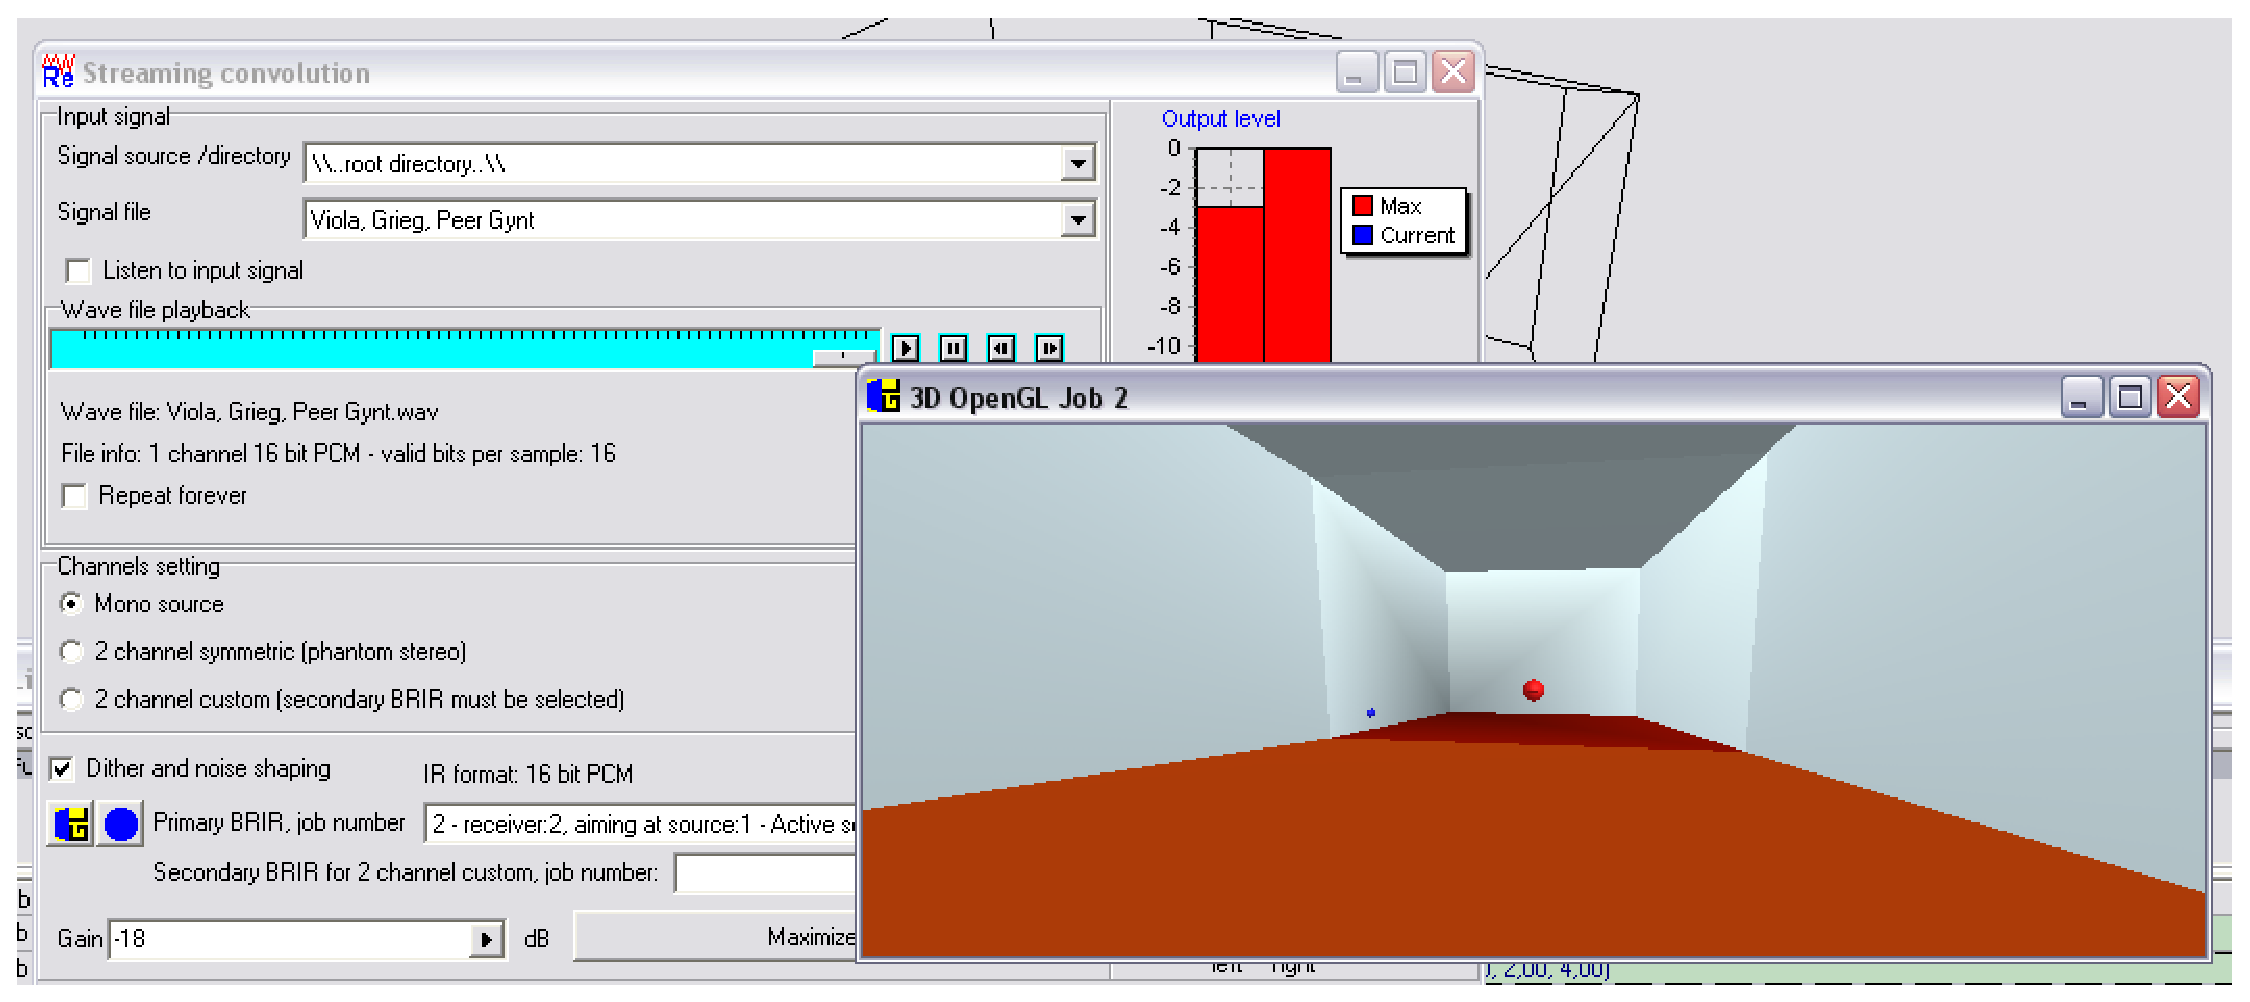
\includegraphics[width=16cm,angle=0]{images/odeon/image6.eps}

{\small{\bf Simulaci�n con Odeon}}
\end{figure}

\clearpage
\pagebreak

\bOpage{introcolor}{0.25}{TUTORIAL}





En la parte inferior se puede seleccionar el otro trabajo, se puede
disminuir la ganancia si el volumen est� muy alto (o aumentarla en
caso contrario) y se puede ver la sala desde la posici�n del receptor
como si estuvi�ramos en la sala adem�s de escuch�ndola (eso s�, con
gr�ficos bastante pobres). 





Ahora pod�is probar a cambiar materiales o fuentes en la sala. Por
ejemplo pod�is coger en uno entre el 907 y el 909  para la zona de
audiencia que simular�a la sala con gente. O pod�is probar a meter un
material m�s absorbente en la pared posterior para comprobar como
pierde fuerza el oyente trasero. 

Incluso os recomiendo probar otras salas de las de demostraci�n que
las hay muy interesantes. Pod�is ver si est�n m�s enfocadas a m�sica o
a oratoria... o incluso intentar mejorarlas para una de las dos
funciones. 



\sectiontext{white}{black}{�Y QUE M�S PUEDO HACER?}

Para abrir un poco m�s el apetito ac�stico vamos a realizar un ultimo
experimento. Abre una de las salas predefinidas distinta a la Example,
por ejemplo el Hagia Irene. Abre la Job List y aparecer�n ya un mont�n
de trabajos predefinidos y en algunas salas como esta, ya calculados
(en verde). Adem�s de escuchar como hicimos antes, pod�is pulsar en la
opci�n View Grid Response del men� Job List. Aparece una maya de
colores sobre el edificio que representan los niveles de alg�n
par�metro. Estos par�metros se cambian con los cursores hacia arriba y
abajo y en frecuencia con los cursores izquierda y derecha.  Algunos
par�metros de f�cil explicaci�n son: 

\begin{itemize}

\item {\bf SPL:} Potencia sonora
\item {\bf T30:} una medida del tiempo de reverberaci�n (distinta a la estad�stica que vimos)
\item {\bf LF:} Eficiencia Lateral. Es una relaci�n entre el sonido que viene frontalmente (directo) y lateralmente (normalmente reflexiones). 
\item {\bf STI:} Indice de transmisi�n del habla. Indica si se entiende bien al oyente. Puede tomar valores de 0 (no se entiende nada) a 1 (se entiende de maravilla). Las reflexiones estropean el par�metro.

\end{itemize}

Y con todos estos par�metros seguramente os preguntar�is: ``Muy bien,
muy bien, pero yo quiero dise�ar una sala fabulosa �C�mo tienen que
estar esos par�metros?'' Bueno, como buen gallego la respuesta es
``Depende �Para que la vas a usar?''. No se si alguno de los lectores
se habr� fijado pero en muchas ocasiones cuando va a una conferencia
en una sala determinada la oratoria se oye relativamente mal, es decir,
las frases del orador no se entienden demasiado bien y, sin embargo,
si hab�is escuchado m�sica en dicha sala es posible que os haya
gustado como suena. 

Este problema est� relacionado con la reverberaci�n del sonido y es
complicado conseguir una ``sala perfecta'' para todo tipo de
uso. Cuanta m�s reverberaci�n tenga una sala, peor es la calidad de
dicha sala para la oratoria. Par�metros relacionados con la
inteligibilidad (comprensi�n) de la palabra como el STI caen de forma
estrepitosa cuanto mayores sean las reflexiones. Es decir, se entiende
mal a un orador. 


Esto es l�gico si pensamos que el eco es una forma retardada del
sonido, entonces si un orador dice dos palabras seguidas como ``!
Buenos d�as!'' y resulta que en la sala en la que estamos escuchando
hay un cierto nivel de eco, el ``Buenos'' lo oiremos bien, pero
resulta que al mismo tiempo que o�mos la versi�n directa del ``d�as''
nos llega la versi�n retardada del ``buenos'' que ser� m�s molesto y
har� que se entienda peor cuanto m�s potente sea dicho eco. Si esto lo
extrapolamos a una charla completa, puede llegar a no entenderse nada
de lo que se dice.  

Sin embargo, si disminuimos mucho la reflexi�n de las superficies de
la sala y tratamos de dar alg�n tipo de concierto musical en la misma
vamos a notar que el sonido est� ``apagado'' sin fuerza. Un cierto
nivel de reverberaci�n para la m�sica (ojo, tampoco debe ser excesiva)
va a provocar un sonido m�s envolvente, con mayor ``calidez''.  De ah�
que sea complicado realizar una sala multiusos. 


Entonces �c�mo podemos mejorar una sala o simplemente una habitaci�n?
Pues lo m�s sencillo y econ�mico normalmente es el cambio de
materiales en las distintas superficies. �No! No hace falta que tir�is
las paredes. Se puede disminuir los ecos en una sala con mucha rever
metiendo unas buenas cortinas en lugares estrat�gicos. O si me quiero
montar un estudio casero puedo utilizar hueveras para cubrir las
paredes ya que simulan (aunque remotamente) a una sala anecoica (que
absorbe muy bien los distintos ecos de los instrumentos
usados). Adem�s, cuando se realza una grabaci�n es muy f�cil
introducir digitalmente los distintos efectos de rever que puedan
interesar para un acabado ``ideal''.

Si por el contrario lo que quiero es aumentar dicha reverberaci�n ya
dependemos un poco m�s de c�mo est� construida y de qu� materiales
consta. Quiz� llegue con sacar esas cortinas del fondo y dejar los
cristales a la vista ya que el sonido lo refleja much�simo m�s un
cristal que una cortina (y adem�s las cortinas eran horrorosas, as�
que dos p�jaros de un tiro). O quitar algunos elementos de la sala si
la tenemos recargada con muchos muebles o recovecos por los que se
pueda perder el sonido.  

Se podr�a escribir un libro m�s que un art�culo si quisi�ramos
explorar todo lo que permite este programa. Para empezar habr�a que
adentrarse en la ac�stica y definir muchos m�s par�metros y conceptos
para luego ponerlos en pr�ctica sobre el programa. Qui�n sabe,  quiz�
en un futuro art�culo avancemos un poco m�s. 



\end{multicols}

\colorbox{introcolor}{
\begin{minipage}{.98\linewidth}
{\footnotesize\sf
{\color{white}{\textbf{BIBLIOGRAF�A}}}

Ingenier�a Ac�stica. M. Sobreira, E. Alexandre. Servicio de
Publicaciones de Teleco Vigo. 2003.

Apuntes de Laboratorio de Ac�stica Arquitect�nica. Sin editar.

http://www.wikipedia.org  (Versi�n inglesa y espa�ola) y http://www.odeon.dk/
}
\end{minipage}
}

\clearpage
\pagebreak

% Este fichero es parte del N�mero 3 de la Revista Occam's Razor
% Revista Occam's Razor N�mero 3
%
% (c)  2007, 2008, The Occam's Razor Team
%
% Esta obra est� bajo una licencia Reconocimiento 2.5 Espa�a de Creative
% Commons. Para ver una copia de esta licencia, visite 
% http://creativecommons.org/licenses/by/2.5/es/
% o envie una carta a Creative Commons, 171 Second Street, Suite 300, 
% San Francisco, California 94105, USA.

% Seccion Historia
%
% Incluye imagen del art�culo


\rput(8.5,-3.8){\resizebox{18cm}{!}{{\epsfbox{images/historia/gauss.eps}}}}

% -------------------------------------------------
% Cabecera
\begin{flushright}
\msection{introcolor}{black}{0.25}{HISTORIA}

\vspace{6.8cm}

{\psset{linecolor=black,linestyle=dotted}\psline(-12,0)}
\end{flushright}

\vspace{2mm}
% -------------------------------------------------

\begin{multicols}{2}


% Introducci�n
\intro{introcolor}{S}{i record�is el primer art�culo que escrib� para
  Occam's Razor, se titulaba ``Mi Historia de las
  Telecomunicaciones''. En aquel texto ya se mencionaba que el primer
  sistema de telecomunicaci�n de la historia fue el tel�grafo
  construido por los f�sicos C. F. Gauss y W. Weber en 1822. 
}

\vspace{2mm}

% Cuerpo del art�culo

  Este
  art�culo pretende describir aquel primitivo sistema esperando que su
  comprensi�n os resulte tan interesante como a m�. Debo comentar que
  el inter�s por el tema procede del se�or Gonzalo Barrio (licenciado
  en f�sica y empleado de la Fundaci�n Empresa Universidad Gallega,
  Feuga, www.feuga.es). Gonzalo est� realizando su tesis doctoral en
  un programa de la Universidad de Santiago llamado ``Historia de la
  Ciencia y la Tecnolog�a'' y decidi� encaminar sus esfuerzos a
  investigar la labor del gran genio alem�n. Una parte de ese trabajo
  es la que describe este art�culo: el estudio y descripci�n del
  funcionamiento del tel�grafo de Gauss y Weber. Cuando Gonzalo me
  pidi� que colaborara en su trabajo, me sent� halagado por su
  confianza en que encontrar�amos la soluci�n pero ante la poca
  informaci�n t�cnica disponible yo no pensaba que acabar�amos
  resolviendo el problema. 


Nuestra primera fuente de informaci�n sobre el tel�grafo de Gauss fue esta foto (procedente del museo dedicado a Gauss en Gottingen, la ciudad donde trabaj� Gauss durante m�s tiempo y donde muri� en 1855).

\end{multicols}


\begin{figure}[ht]
\centering
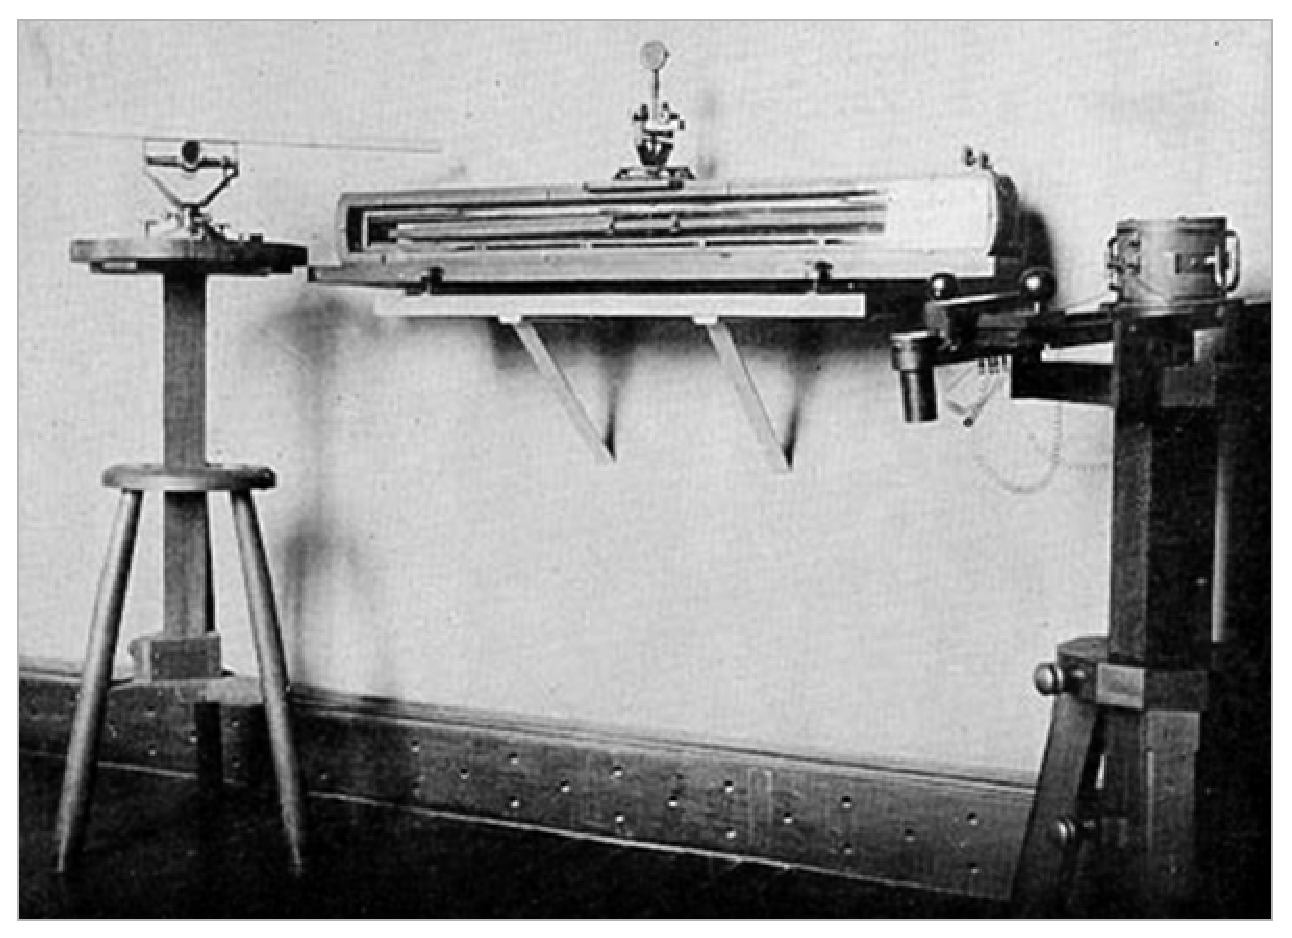
\includegraphics[width=13.0cm,angle=0]{images/historia/gauss-image1.eps}

{\bf Figura 1. Tel�grafo de Gauss}
\end{figure}



\clearpage
\pagebreak


\msection{introcolor}{black}{0.25}{HISTORIA}

\begin{multicols}{2}

Desde luego s�lo con esta foto era imposible saber nada. Despu�s logramos m�s informaci�n: m�s fotos procedentes del mismo museo, una carta de Gauss comentando sus pruebas al astr�nomo Olbers y tambi�n el CD ``Genial Gauss Gottingen'', editado en Alemania para conmemorar el 250 aniversario de su muerte.

\sectiontext{white}{black}{EL TEL�GRAFO DE MORSE}

Nunca hubi�ramos entendido el tel�grafo de Gauss sin haber examinado
primero el de Morse (posterior). El siguiente esquema pertenece a un
tel�grafo de la �poca de Morse y es mucho m�s comprensible porque ya
es un esquema el�ctrico:


\myfig{0}{images/historia/gauss-image2.eps}{1}
\begin{center}
{\footnotesize\bf Figura 2. El tel�grafo de Morse}
\end{center}

\medskip

Vemos que el emisor se basa en una bater�a y un pulsador. El negativo est� conectado permanentemente a tierra y el pulsador permite aplicar tensi�n o no a la l�nea. Si pulsamos durante un segundo tendremos un pulso de tensi�n en la l�nea... una se�al as�:

\begin{center}
\myfig{0}{images/historia/gauss-image3.eps}{1}

{\footnotesize\bf Figura 3. Pulso de tensi�n generado por una pila y un conmutador.}
\end{center}


Ese pulso va a viajar hasta el otro lado (porque el hilo met�lico y la
tierra forman una l�nea de transmisi�n. 

Una vez que el pulso llega a la bobina del electroim�n se generar� una
fuerza magn�tica que atraer� a la pieza met�lica que sostiene el
punz�n. Eso har� que se escriba sobre el papel durante el tiempo que
se ha apretado el pulsador. Como el rollo de papel est� continuamente
en movimiento, si pulsamos s�lo un instante el receptor obtiene un
punto (se ha transmitido un pulso corto). Si pulsamos durante un poco
m�s de tiempo se transmitir� un pulso m�s largo y el receptor obtendr�
una raya. Con eso ya se ha conseguido una comunicaci�n puesto que 
somos capaces de enviar dos s�mbolos diferentes. El tel�grafo de Morse
usa, por tanto, una modulaci�n temporal (la informaci�n va en la
duraci�n de las se�ales). 

\bigskip

{\colorbox{excolor}{
\begin{minipage}{0.98\linewidth}
Adem�s, como sabr�is, Morse desarroll� un c�digo prefijo �ptimo con 26
s�mbolos (las letras del alfabeto). Se trata de un c�digo de longitud
variable m�s evolucionado que los de longitud fija (Gauss y Weber
usaban palabras c�digo de 5 bits para un alfabeto de 32 mensajes
posibles). Para poder decodificar un c�digo de longitud variable se
debe cumplir que ninguna palabra c�digo sea prefijo de otra (c�digo
prefijo). Adem�s, es un c�digo de entrop�a m�nima (las palabras c�digo
m�s cortas corresponden a los s�mbolos m�s probables logrando una
longitud media �ptima desde un punto de vista estad�stico). {\bf El m�todo
matem�tico para crear c�digos prefijo �ptimos no se conoci� hasta que
lo desarroll� Huffman en 1952. �M�s de cien a�os despu�s!}
\end{minipage}
}}

\bigskip

{\colorbox{introcolor}{
\begin{minipage}{0.98\linewidth}
Wilhem Weber (1804-1891) fue un f�sico alem�n recordado por sus trabajos sobre el campo magn�tico. De hecho, hoy en d�a a la unidad de flujo magn�tico se le llama Weber. Weber lleg� a ser profesor de f�sica en Gottingen con s�lo 27 a�os. Gauss comenz� a colaborar con �l al ver que era un cient�fico de su nivel y juntos desarrollaron varios trabajos. La capacidad de Gauss para idear nuevos artefactos se complementaba muy bien con la capacidad pr�ctica de Weber para crearlos y probarlos.
\end{minipage}
}}

\bigskip

{\colorbox{excolor}{
\begin{minipage}{0.98\linewidth}
El primer mensaje telegr�fico de la historia lo recibi� Weber y dec�a
textualmente: {\tt Michelman kommt} (``Michelman viene'' en alem�n). En �l Gauss informaba a Weber de que su com�n ayudante Michelman hab�a salido del observatorio (donde trabajaba Gauss) en direcci�n a la facultad de f�sica (lugar de trabajo de Weber).
\end{minipage}
}}

\sectiontext{white}{black}{EL TEL�GRAFO DE GAUSS}

A partir del tel�grafo de Morse y de la informaci�n disponible dedujimos que el tel�grafo de Gauss respond�a a un esquema el�ctrico como �ste:

\begin{center}
\myfig{0}{images/historia/gauss-image4.eps}{1}

{\footnotesize\bf Figura 4. Esquema El�ctrico del Tel�grafo de Gauss.}
\end{center}

\ebOpage{introcolor}{0.25}{HISTORIA}

El emisor consiste en alg�n tipo de generador o acumulador de energ�a
(Gauss en su carta a Olbers le llama ``pila voltaica''). De hecho, en
las fotos se ve un objeto cil�ndrico con aspecto de primitivo
condensador que podr�a ser usado para acumular la tensi�n que va a
generar los pulsos (podr�a ser un dispositivo muy similar a la botella
de Leyden que ya se conoc�a desde 1746, pod�is ver una descripci�n
sencilla en: {\small \verb!http://es.wikipedia.org/wiki/Botella_de_Leyden!})

\begin{center}
\myfig{0}{images/historia/gauss-image5.eps}{0.3}

{\footnotesize\bf Figura 5. Emisor.}
\end{center}

El c�digo de Gauss y Weber se basaba en mover la aguja receptora
(horizontal aunque en el esquema aparece vertical) a la izquierda o a
la derecha, de modo que la modulaci�n de la se�al se va a basar en su
signo (es una modulaci�n en amplitud y no temporal como la del
tel�grafo de Morse). De esta forma, la conexi�n de la pila emisora a
la l�nea ten�a que consistir en un interruptor relativamente complejo
(Gauss le llama ``conmutador'') que permitiera tres estados:

\begin{itemize}
\item {\bf Neutro}: el operador no hace nada los dos bornes de la pila est�n abiertos.
\item {\bf Enviando pulso positivo}: el operador ordena mover la aguja receptora a la derecha  el borne positivo se une a la l�nea y el negativo a tierra. Se env�a un pulso positivo (su duraci�n no es importante pero ser� el tiempo que el operador mantiene el pulsador en esta posici�n):

\begin{center}
\myfig{0}{images/historia/gauss-image6.eps}{0.8}

{\footnotesize\bf Figura 6. Pulso Positivo.}
\end{center}

\item {\bf Enviando pulso negativo}: el operador ordena mover la aguja receptora a la izquierda el borne positivo se une a tierra y el negativo a la l�nea. Se env�a un pulso opuesto al de Morse:

\begin{center}
\myfig{0}{images/historia/gauss-image7.eps}{0.8}

{\footnotesize\bf Figura 7. Pulso Negativo.}
\end{center}


\end{itemize}

N�tese que pulsos opuestos generar�n campos magn�ticos tambi�n
opuestos y movimientos de la aguja hacia un lado o a otro. En el CD se
dispone de figuras de un manuscrito que detalla el c�digo original y
se ve que lo que hoy llamar�amos bits aparece codificado con los
signos ``+'' y ``-'' en vez de ``1'' y ``0''.

\end{multicols}

\begin{figure}[ht]
\centering
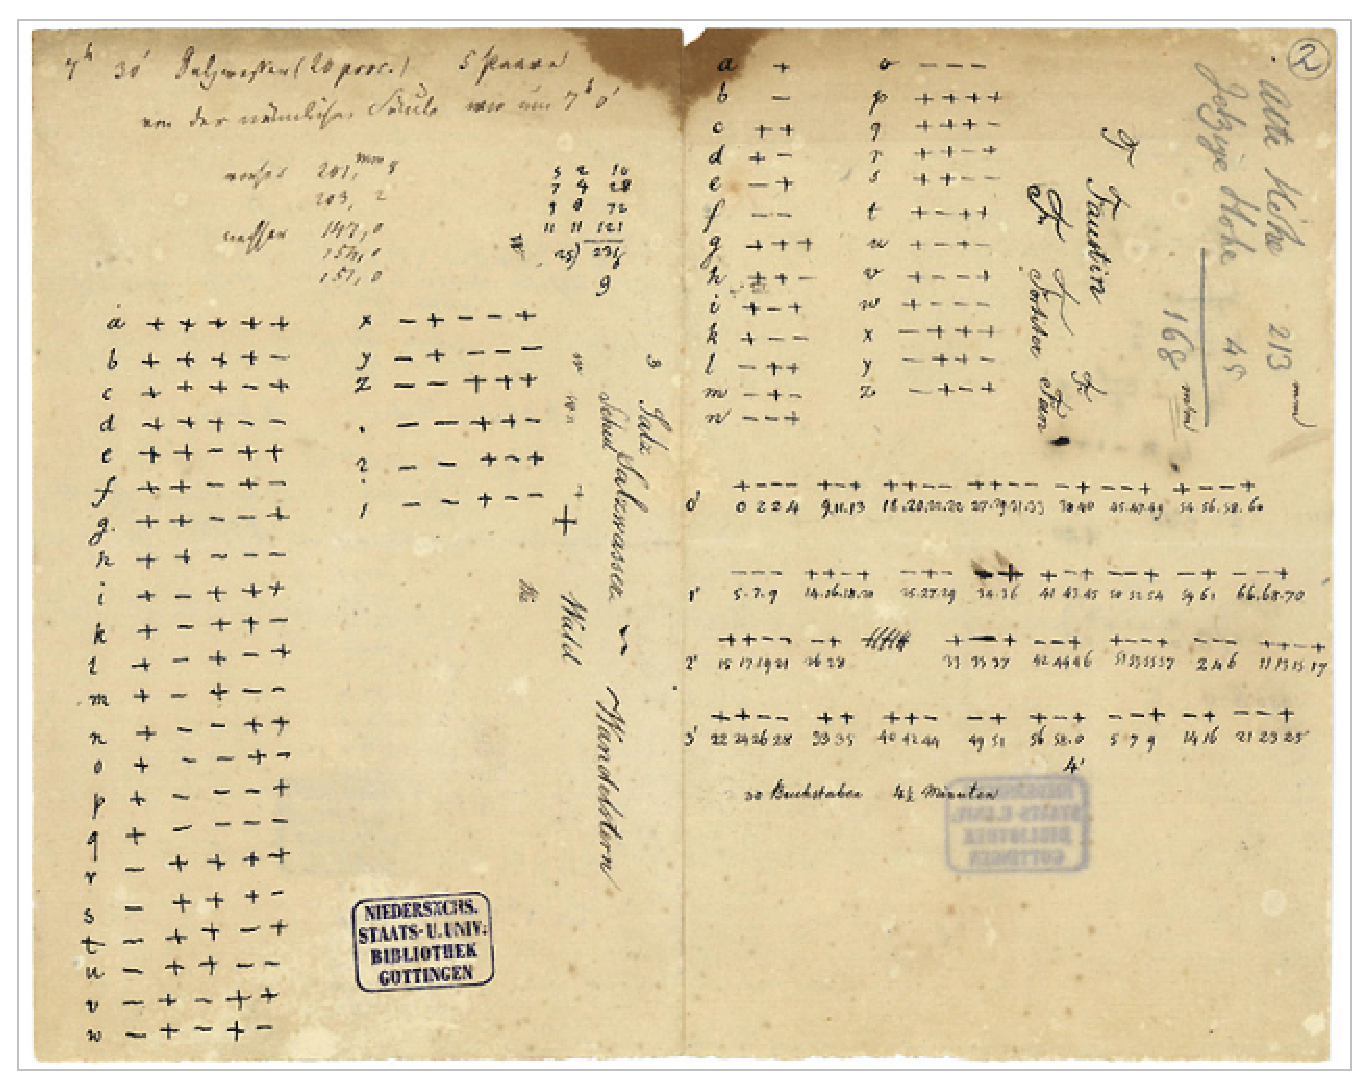
\includegraphics[height=10.0cm,angle=0]{images/historia/gauss-image10.eps}

{\footnotesize\bf Figura 8. C�digo Original.}
\end{figure}

\clearpage
\pagebreak

\bOpage{introcolor}{0.25}{HISTORIA}

El receptor posee una bobina y una aguja imantada. Gauss le llama
galvan�metro y, de hecho, es un dispositivo similar a los medidores de
D'Arsonval (desarrollados por Jacques-Ars�ne d'Arsonval en el siglo
XIX) con disposici�n de la aguja horizontal en vez de estar montada
sobre un cuerpo giratorio (otra diferencia es que en el medidor de
D'Arsonval el im�n es fijo y la bobina es m�vil). 

En este tel�grafo era necesario un anteojo para ver las desviaciones
de la aguja que deb�an de ser muy d�biles. Lo que no es de extra�ar si
se usaba un condensador como fuente de energ�a: se generaba un pulso
no muy potente que deb�a atravesar m�s de dos kil�metros de un cable
que seguramente ten�a una atenuaci�n por metro muy alta (existe un
dibujo del tendido inicial realizado sobre los tejados, esta
instalaci�n un�a el laboratorio de Gauss con el de Weber). Otra raz�n
es el gran peso de la aguja (Gauss habla de un im�n de una libra) y el
hecho de si se pudo incluir o no un n�cleo de hierro en el interior de
la bobina. De incluirse, el campo magn�tico es mucho mayor, Gauss habla
de una bobina de 50 vueltas y no dice nada sobre un n�cleo, incluirlo
parece dif�cil si tiene que haber una aguja dentro. 

\begin{center}
\myfig{0}{images/historia/gauss-image8.eps}{1}

{\footnotesize\bf Figura 9. Bobina receptora (izquierda). Anteojo usado para ver el movimiento de la aguja.}
\end{center}

\sectiontext{white}{black}{CONCLUSIONES}

Como conclusi�n final pensad que podemos establecer a Gauss y Weber
como los padres de las telecomunicaciones. Su prototipo no fue muy
tenido en cuenta en su pa�s, a diferencia del de Morse que logr� el
inter�s del gobierno norteamericano de la �poca. Despu�s vinieron
otros muchos sistemas (ved, por ejemplo, el dossier sobre el tema en
el primer n�mero de Occam's Razor). 

Como conclusiones m�s personales a ambos nos ha parecido apasionante
escudri�ar en la historia para intentar explicar el funcionamiento de
viejos pero ingeniosos sistemas. Es una faceta investigadora un poco
diferente a las habituales pero igualmente gratificante. 


\end{multicols}


\begin{figure}[ht]
\centering
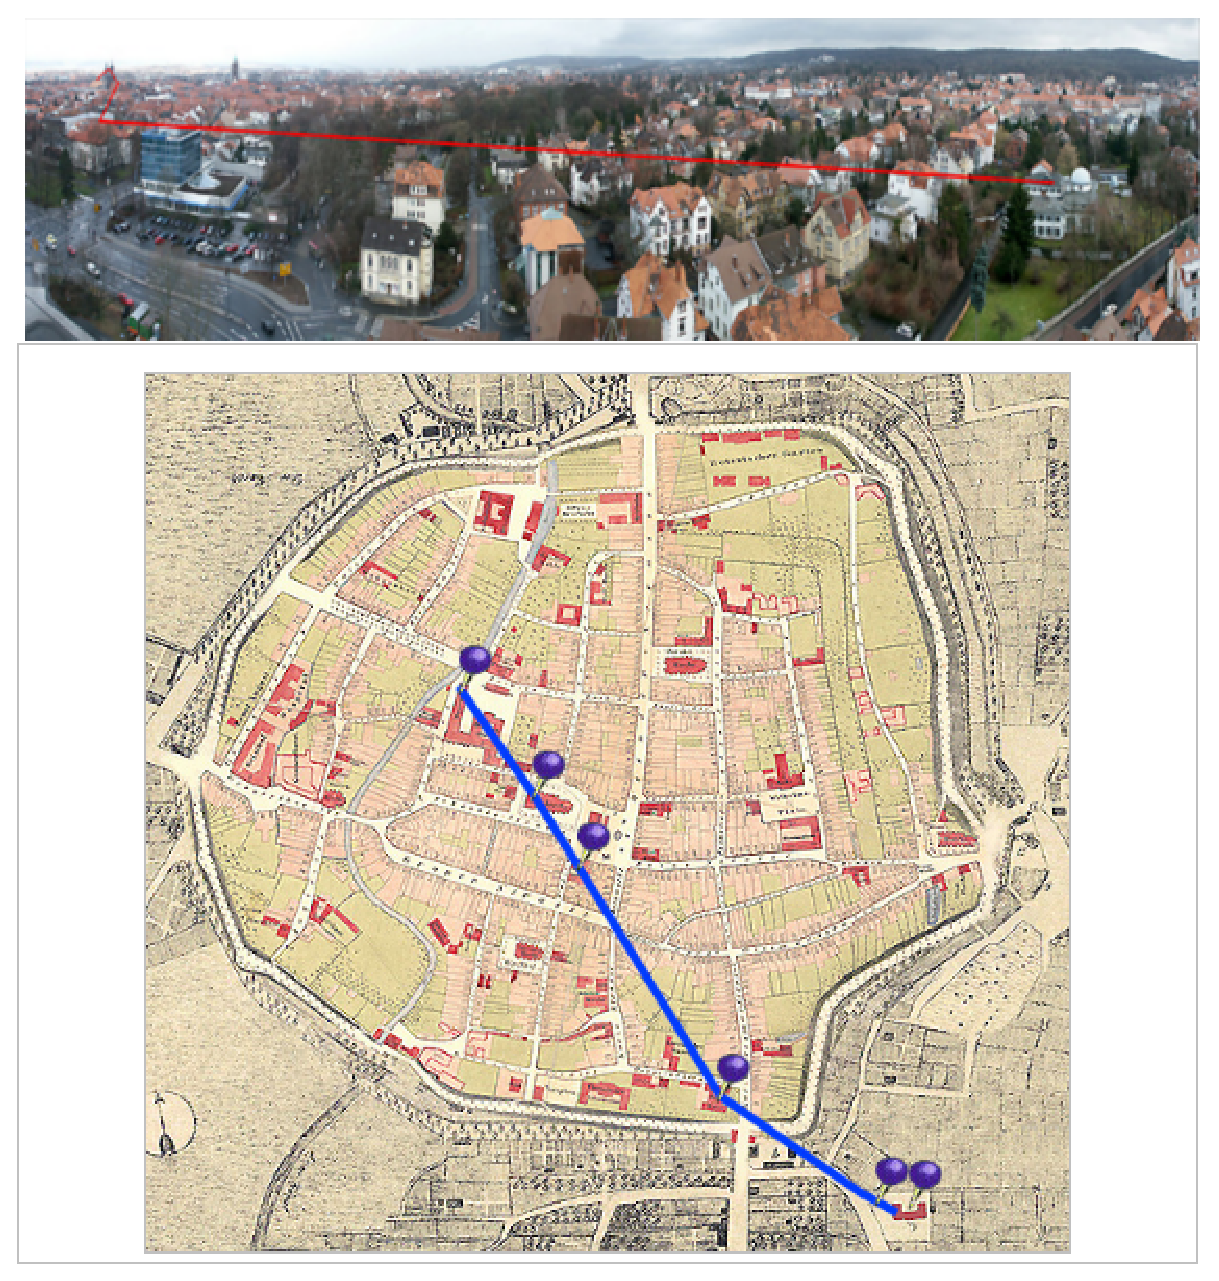
\includegraphics[height=12.0cm,angle=0]{images/historia/gauss-image9.eps}

{\footnotesize\bf Figura 10. Tendido inicial. Arriba: puntos inicial y final (laboratorio de f�sica de Weber a la izquierda, observatorio astron�mico de Gauss a la derecha). Abajo: mapa de la �poca detallando el recorrido del cable.}
\end{figure}



\clearpage
\pagebreak

% Este fichero es parte del N�mero 3 de la Revista Occam's Razor
% Revista Occam's Razor N�mero 3
%
% (c)  2007, 2008, The Occam's Razor Team
%
% Esta obra est� bajo una licencia Reconocimiento 2.5 Espa�a de Creative
% Commons. Para ver una copia de esta licencia, visite 
% http://creativecommons.org/licenses/by/2.5/es/
% o envie una carta a Creative Commons, 171 Second Street, Suite 300, 
% San Francisco, California 94105, USA.

% Seccion Reverso Tenebroso
%
% Incluye imagen del art�culo


\rput(1,-2.4){\resizebox{!}{6cm}{{\epsfbox{images/reverso/cage.eps}}}}

% -------------------------------------------------
% Cabecera
\begin{flushright}
\msection{introcolor}{black}{0.35}{REVERSO TENEBROSO}

\mtitle{10cm}{Poniendo Contrase�as a Ejecutables}

\msubtitle{11cm}{O como parchear el segmento .note.ABI-tag}

{\sf por Er de la Secci�n}

{\psset{linecolor=black,linestyle=dotted}\psline(-12,0)}
\end{flushright}

\vspace{2mm}
% -------------------------------------------------

\begin{multicols}{2}


% Introducci�n
\intro{introcolor}{C}{uando se dispone del c�digo fuente de una
  determinada aplicaci�n (como sucede en los sistemas libres), a�adir
  una contrase�a a cualquiera de ellos para no permitir su uso por
  desconocidos es sencillo. Pero cuando el c�digo fuente no est�, la cosa
  es un poco m�s... interesante.
}

\vspace{2mm}

% Cuerpo del art�culo

En este art�culo vamos a describir una sencilla t�cnica para parchear
ejecutables. El ejemplo que utilizaremos, proteger con una contrase�a,
no es que sea especialmente �til, pero es una de las cosas m�s
sencillas que podemos hacer para ilustrar el proceso. 

Una vez sep�is como funciona todo esto, estamos seguros de que se os
ocurrir�n montones de ideas interesantes con las que divertiros
parcheando ejecutables. Bien, vamos a ello.



% Introducci�n al formato ELF
\sectiontext{white}{black}{EL FORMATO ELF}

El formato ELF (Executable and Linkable Format o formato ejecutable y
enlazable), es el formato utilizado por la mayor�a de los sistema UNIX
para sus programas, es decir, todo ejecutable en nuestro sistema se
almacena en el disco utilizando este formato (bueno, podemos utilizar
otros formatos, pero no es lo habitual).

Cuando compilamos nuestros programas a partir del c�digo fuente, en el
lenguaje que m�s rabia nos d�, iniciamos un proceso bastante complejo
que termina cuando nuestro programa est� cargado en memoria. 

S�, vale, tras compilar nuestro programa obtenemos un fichero
ejecutable en el disco y parece que ah� se termina todo, sin embargo,
el sistema todav�a tiene que hacer unas cuantas cosas al cargarlo en
memoria para que ese fichero se convierta en la imagen de un proceso
en ejecuci�n.

\begin{entradilla}
{\em {\color{introcolor}ELF es el formato ejecutable} m�s com�n en los sistemas UNIX}
\end{entradilla}


As�, el fichero que almacenamos en disco es el resultado del proceso
de enlazado (link), pero el proceso de carga para su ejecuci�n,
requiere que el sistema lleve a cabo ciertas operaciones como la
relocalizaci�n de c�digo o la carga de librer�as din�micas externas y
su enlazado en tiempo de ejecuci�n. Estas tareas las realiza el
denominado enlazador din�mico (dynamic linker en ingl�s :).


Nosotros, en este art�culo, vamos a trabajar sobre los ficheros
ejecutables. B�sicamente vamos a hacer de enlazadores, a�adiendo
c�digo a un fichero ELF, y modific�ndolo para que, cuando el programa
se cargue en memoria y el enlazador din�mico lleve a cabo su tarea,
todo est� correcto.

% Cabecera y Punto de Entrada
\sectiontext{white}{black}{CABECERA Y PUNTO DE ENTRADA}

Como suele ser habitual, los formatos de fichero suelen tener una
cabecera. Esta cabecera nos proporciona informaci�n para verificar que
el fichero es de ese formato y para acceder al resto de informaci�n
que el fichero contiene.

Pues bien, el formato ELF empieza con una peque�a cabecera. 

Antes de continuar, permitirnos hacer un peque�o comentario. En este
art�culo no vamos a describir todos los detalles del formato ELF,
solamente aquellos que tengan que ver con el tema que nos ocupa. Los
que est�is interesados en conocer todos los detalles sobre ELF (merece la pena)
deber�is descargaros la especificaci�n de este formato, la cual
encontr�is f�cilmente en Internet. 

Tras este breve inciso, veamos la cabecera t�pica de un ejecutable
ELF. Para ello vamos a utilizar la herramienta readelf, que nos
permite visualizar la informaci�n interna de los ficheros de una forma
sencilla.

{\scriptsize
\begin{verbatim}
occam@razor: $ readelf -h /bin/ls
ELF Header:
  Magic:   7f 45 4c 46 01 01 01 00 00 00 00 00 00 00 00 00 
  Class:                             ELF32
  Data:                              2's complement, little endian
  Version:                           1 (current)
  OS/ABI:                            UNIX - System V
  ABI Version:                       0
  Type:                              EXEC (Executable file)
  Machine:                           Intel 80386
  Version:                           0x1
  Entry point address:               0x8049b40
  Start of program headers:          52 (bytes into file)
  Start of section headers:          76752 (bytes into file)
  Flags:                             0x0
  Size of this header:               52 (bytes)
  Size of program headers:           32 (bytes)
  Number of program headers:         8
  Size of section headers:           40 (bytes)
  Number of section headers:         27
  Section header string table index: 26

\end{verbatim}
%$
}

De todos esos campos en la cabecera del fichero a nosotros nos van a
interesar dos de ellos. El primero, como os pod�is imaginar es la {\em
  Direcci�n del Punto de Entrada} (Entry Point Address). 

Este campo nos dice cual es la direcci�n de memoria en la que empezar� la
ejecuci�n del programa, una vez haya sido cargado y procesado.

\ebOpage{introcolor}{0.35}{REVERSO TENEBROSO}

El segundo campo que nos va a interesar es el desplazamiento del {\em
  Comienzo de las cabeceras de programas} (Start of program
  headers). En seguida veremos que esto.

% Secciones y Segmentos 
\sectiontext{white}{black}{SECCIONES}

El formato ELF, organiza toda la informaci�n que el sistema necesita
para poder ejecutar un programa en dos estructuras principales:
secciones y segmentos.

Las primeras, las secciones, realmente contienen pistas y ayudas para
los cargadores de programas, depuradores, etc... 

Veamos que apariencia tienen las secciones de nuestro querido
\verb!/bin/ls!:

{\scriptsize
\begin{verbatim}
occam@razor: $ readelf -S /bin/ls
There are 27 section headers, starting at offset 0x12bd0:

Section Headers:
  [Nr] Name              Type          Addr     Off    Size   
  [ 0]                   NULL          00000000 000000 000000 
  [ 1] .interp           PROGBITS      08048134 000134 000013 
  [ 2] .note.ABI-tag     NOTE          08048148 000148 000020 
  [ 3] .hash             HASH          08048168 000168 000340 
  [ 4] .dynsym           DYNSYM        080484a8 0004a8 0006d0 
  [ 5] .dynstr           STRTAB        08048b78 000b78 0004bb 
  [ 6] .gnu.version      VERSYM        08049034 001034 0000da 
  [ 7] .gnu.version_r    VERNEED       08049110 001110 0000c0 
  [ 8] .rel.dyn          REL           080491d0 0011d0 000028 
  [ 9] .rel.plt          REL           080491f8 0011f8 000308 
  [10] .init             PROGBITS      08049500 001500 000017 
  [11] .plt              PROGBITS      08049518 001518 000620 
  [12] .text             PROGBITS      08049b40 001b40 00cec8 
  [13] .fini             PROGBITS      08056a08 00ea08 00001c 
  [14] .rodata           PROGBITS      08056a40 00ea40 003c2f 
  [15] .eh_frame_hdr     PROGBITS      0805a670 012670 00002c 
  [16] .eh_frame         PROGBITS      0805a69c 01269c 0000ac 
  [17] .ctors            PROGBITS      0805b748 012748 000008 
  [18] .dtors            PROGBITS      0805b750 012750 000008 
  [19] .jcr              PROGBITS      0805b758 012758 000004 
  [20] .dynamic          DYNAMIC       0805b75c 01275c 0000e0 
  [21] .got              PROGBITS      0805b83c 01283c 000008 
  [22] .got.plt          PROGBITS      0805b844 012844 000190 
  [23] .data             PROGBITS      0805b9e0 0129e0 00010c 
  [24] .bss              NOBITS        0805bb00 012aec 000430 
  [25] .gnu_debuglink    PROGBITS      00000000 012aec 000008 
  [26] .shstrtab         STRTAB        00000000 012af4 0000db 
\end{verbatim}
%$
}

Por cuestiones de espacio hemos eliminado las �ltimas columnas de la
salida del comando, ya que no no nos son de utilidad. Aunque para
parchear nuestro programa trabajaremos casi exclusivamente con los
segmentos del programa, pero un par de comentarios sobre las secciones
son necesarios... para que os pique la curiosidad.

Lo primero que hay que comentar es que las secciones tienen nombre, y
espero que os hay�is fijado en el nombre de una de las primeras que os
deber�a sonar, a no ser, claro, que se�is de esas personas que no leen
los t�tulos de los art�culos :).

\begin{entradilla}
{\em Las {\color{introcolor}secciones de tipo PROGBITS} son las que se encuentran
  realmente en el fichero}
\end{entradilla}

Lo segundo es que hay varios tipos de secciones. Ya sab�is, si quer�is
conocer los detalles consultad la especificaci�n. En lo que a
nosotros respecta, el tipo interesante es PROGBITS. 

Todas las
secciones de este tipo, se encuentran f�sicamente en el fichero y
ser�n cargadas en la posici�n de memoria que indica la columna Addr,
cuando ejecutemos el programa. Adem�s, la siguiente columna, Off, nos
indica el desplazamiento en el fichero en el que se encuentran los
datos asociados a esa secci�n y que ser�n cargados en la direcci�n de
memoria respectiva.

Sobre la secci�n .note.ABI-tag, volveremos m�s tarde.

% Segmentos
\sectiontext{white}{black}{SEGMENTOS O CABECERAS DE PROGRAMA}

Los segmentos o
cabeceras de programas (Program Headers) son la otra estructura de
datos principal, que el formato ELF maneja. 

Estos segmentos son los que definen la
estructura f�sica real que un determinado programa tendr� en
memoria... es decir, donde y como aparecer� cada parte del programa en
la memoria del ordenador. Lo que se conoce como el mapa de memoria del
proceso. 

Veamos la lista de segmentos de \verb!/bin/ls!:

{\scriptsize
\begin{verbatim}
occam@razor: $ readelf -l /bin/ls

Elf file type is EXEC (Executable file)
Entry point 0x8049b40
There are 8 program headers, starting at offset 52

Program Headers:
  Type         Offset   VirtAddr   PhysAddr   FileSiz MemSiz  Flg Align
  PHDR         0x000034 0x08048034 0x08048034 0x00100 0x00100 R E 0x4
  INTERP       0x000134 0x08048134 0x08048134 0x00013 0x00013 R   0x1
      [Requesting program interpreter: /lib/ld-linux.so.2]
  LOAD         0x000000 0x08048000 0x08048000 0x12748 0x12748 R E 0x1000
  LOAD         0x012748 0x0805b748 0x0805b748 0x003a4 0x007e8 RW  0x1000
  DYNAMIC      0x01275c 0x0805b75c 0x0805b75c 0x000e0 0x000e0 RW  0x4
  NOTE         0x000148 0x08048148 0x08048148 0x00020 0x00020 R   0x4
  GNU_EH_FRAME 0x012670 0x0805a670 0x0805a670 0x0002c 0x0002c R   0x4
  GNU_STACK    0x000000 0x00000000 0x00000000 0x00000 0x00000 RW  0x4

 Section to Segment mapping:
  Segment Sections...
   00     
   01     .interp 
   02     .interp .note.ABI-tag .hash .dynsym .dynstr .gnu.version 
.gnu.version_r .rel.dyn .rel.plt .init .plt .text .fini .rodata 
.eh_frame_hdr .eh_frame 
   03     .ctors .dtors .jcr .dynamic .got .got.plt .data .bss 
   04     .dynamic 
   05     .note.ABI-tag 
   06     .eh_frame_hdr 
   07     
\end{verbatim}
%$
}

Por cuestiones de espacio hemos eliminado la �ltima columna de la
salida del programa. Esta columna define la alineaci�n de cada uno de
los segmentos (byte, palabra, p�gina,...), para nuestro cometido, no
necesitamos esta informaci�n, pero existen otras t�cnicas de parcheado
de binarios que si la requieren.

Lo primero que vemos es que la lista de segmentos es mucho m�s peque�a
y adem�s, que estos no tienen nombre. La utilidad {\tt readelf} nos
proporciona un mapeado de secciones y segmentos al final de la
salida. 

Estos mapeados se determinan a partir de las direcciones de secciones y
segmentos del tama�o de los segmentos. Pod�is hacer la prueba vosotros
mismos.

\ebOpage{introcolor}{0.35}{REVERSO TENEBROSO}

El resto de la informaci�n asociada a cada segmento es bastante obvia:
el desplazamiento dentro del fichero donde se encuentran los datos,
las direcciones en las que se crear�n los segmentos y su tama�o en
disco y en memoria.

Observad que en general el tama�o en disco y en memoria son iguales,
excepto para el segmento n�mero 3 (empezamos a contar en 0 :). Si nos
fijamos en las secciones asociadas a ese segmento nos encontramos la
secci�n .bss. Esta secci�n es la que contiene los datos no
inicializados, y por lo tanto, no necesitamos almacenar ninguna
informaci�n en el fichero.

Cuando el programa se carga en memoria, el cargador se encarga de que
haya espacio para esos datos.

% Formato del proceso en Memoria
\sectiontext{white}{black}{MAPA DE MEMORIA DEL PROCESO}

Bien. �Y qu� aspecto tiene todo esto en memoria?. Pues b�sicamente el
que nos ha mostrado readelf cuando le pedimos que nos listara los
segmentos del programa, pero algunos comentarios nos van a ayudar a
comprender la forma en la que parchearemos el programa en breve.

La siguiente figura muestra el mapa de memoria t�pico de un proceso en
el sistema operativo GNU/Linux.

\myfig{0}{images/reverso/mapa-memoria-proceso.eps}{0.5}

Hay dos cosas interesantes en esta figura. La primera es
que, al menos en los sistemas GNU/Linux, los ejecutables se cargan a
partir de una direcci�n f�sica en memoria (0x800440000). Esto va a
hacer nuestra vida mucho m�s sencilla.

La segunda es que el bloque inicial de segmentos (cabecera + c�digo +
datos) se corresponde exactamente con el contenido de nuestro fichero
ejecutable. Esto es as� debido al dise�o del formato ELF, en el que se
pretend�a reducir lo m�s posible las operaciones a realizar para
cargar un proceso en memoria. En la siguiente secci�n veremos como
sacar partido de esto.

Finalmente, observad que en la figura hemos incluido los permisos de
cada segmento (la columna Flg que nos proporciona readelf -l). 

Si os fij�is, el primer segmento es el que contiene el c�digo de
nuestro programa y solamente tiene permisos de lectura (R) y (E), lo
cual es l�gico... no queremos que el programa se pueda modificar o
automodificar... �o s� lo queremos?.

\begin{entradilla}
{\em Los {\color{introcolor}ficheros ELF se cargan directamente en memoria} para su ejecuci�n}
\end{entradilla}

El segundo segmento es el que contiene los datos, variables, secci�n
bss, etc... Este, como es l�gico, se inicializa con permisos de
lectura (R) y escritura (W).

Como es habitual, la pila se sit�a en las posiciones altas de la
memoria y ``crece'' hacia las bajas, y las librer�as din�micas y el
heap (memoria din�mica... malloc y todo eso) utilizar�n la memoria a
continuaci�n de los segmentos que componen el programa, creciendo
hacia las direcciones altas. 

De esta forma cuanto m�s uso hagamos de la memoria din�mica y de la pila, el
hueco entre ambas se ir� haciendo m�s peque�o.



% Parcheando segmentos
\sectiontext{white}{black}{PARCHEANDO EJECUTABLES}

Despu�s de esta ``no corta'' introducci�n vamos al tema que nos
ocupa. Parchear ejecutables.

Existen varias formas de parchear un ejecutable ELF. Animamos a los
interesados en conocer los detalles de las otras alternativas, a leer
los textos de Silvio Cesare... totalmente imprescindibles. Lo que os
hemos contado hasta ahora os resultar� �til para comprender las
distintas t�cnicas que el se�or Cesare explica estupendamente.

Como os dec�amos, nosotros vamos a utilizar la que quiz�s sea la t�cnica
m�s sencilla: el parcheado del segmento .note.ABI-tag.

La t�cnica es muy sencilla, b�sicamente consiste en los siguientes
pasos:

\begin{itemize}
\item Abrir el fichero a parchear 
\item A�adirle al final el c�digo que queremos insertar
\item Localizar el segmento que contiene la secci�n .note.ABI-tag
\item Modificar el segmento para:
\begin{itemize}
\item que el sistema cargue este segmento con el resto
  del programa cuando este es ejecutable
\item Tenga permisos de ejecuci�n
\item Los offsets en memoria y en el disco apunten al c�digo que hemos a�adido
\end{itemize}
\item Modificar el punto de entrada en la cabecera ELF para que la
  ejecuci�n se inicie en el nuevo c�digo insertado
\item A�adir cualquier informaci�n extra que queramos.
\end{itemize}

\ebOpage{introcolor}{0.35}{REVERSO TENEBROSO}

No os preocup�is esto es mucho m�s sencillo de lo que parece :).

\sectiontext{white}{black}{ALGUNAS ACLARACIONES}

Antes de meternos con los fragmentos de c�digo que hacen cada una de
las operaciones que necesitamos, vamos a hacer algunas aclaraciones
sobre el porqu� de que esto se haga de la forma en la que se hace.

Lo primero es porque utilizamos la secci�n .note-ABI.tag. 

Bien, hay
varias razones. La primera es que, al menos en los sistemas GNU/Linux
est� siempre ah�, gcc la genera. 

\begin{entradilla}
{\em {\color{introcolor}A�adir segmentos a un ejecutable es complicado}, as� que
  reutilizamos uno de los existentes}
\end{entradilla}

La segunda, y m�s importante, es que
a�adir un nuevo segmento a un ejecutable es bastante complicado, as�
que nos interesa reutilizar alguno de los que ya existen. El segmento
asociado a la secci�n .note-ABI-tag, ya existe y no tiene ninguna
utilidad en la pr�ctica. Es decir, no vamos a romper el programa si lo
utilizamos para otra cosa.

Utilizar alguno de los otros segmentos ser�a bastante m�s
complicado. Bueno, si nuestro c�digo es peque�o existen trucos, pero
en el caso general no resulta pr�ctico.


\sectiontext{white}{black}{PREPARACI�N}

En nuestro parcheador, utilizamos un par de funciones de ayuda y una
constante. Este primer bloque del listado lo pod�is ver a continuaci�n.

\lstset{language=C,frame=tb,framesep=5pt,basicstyle=\scriptsize}   
\begin{lstlisting}
#include <stdio.h>
#include <stdlib.h>
#include <string.h>

#include <unistd.h>
#include <fcntl.h>
#include <sys/stat.h>

#include <elf.h>
#include <sys/mman.h>

#define ADDRESS 0x08044000 

int get_file_size (int fd)  {
  struct stat _info;
  fstat(fd,&_info);
  return _info.st_size;
}

void PURGATUS_EST (int sys, int cond, char *msg) {
  if (cond) {
      if (sys) 	perror (msg); 
      else fprintf (stderr, "%s\n", msg);
      exit (1);
    }
  return;
}


\end{lstlisting}

S�, existe un fichero elf.h que nos va a hacer nuestra vida m�s f�cil
a la hora de leer cabeceras y modificar segmentos.

Adem�s necesitaremos algunas variables en nuestra funci�n main.

\lstset{language=C,frame=tb,framesep=5pt,basicstyle=\scriptsize}   
\begin{lstlisting}
int main (int argc, char *argv[]) {
  void           *data;
  int            size, size1;
  int            fd, fd1;
  int            i;
  Elf32_Ehdr     *elf_hdr;
  Elf32_Phdr     *elf_seg;
  unsigned char  *code;

  PURGATUS_EST (0, argc!=4, 
               "Usar: ./note-patch exe codigo clave");
\end{lstlisting}

Lo primero que hace nuestro programa es comprobar que recibe el n�mero
de par�metros correctos. Tal y como lo hemos programado, el programa
espera como primer par�metro el nombre del ejecutable a parchear, como
segundo par�metro, el c�digo que queremos insertar (m�s tarde veremos
como generarlo) y finalmente la clave.

Si record�is, lo que pretend�amos hacer era poder a�adir una clave a
cualquier ejecutable en nuestro sistema, deforma que si la clave
correcta no es proporcionada, el programa no se ejecuta. Bien, esa
clave la grabaremos a fuego y sangre al parchear el ejecutable.

% Modificando ficheros. mmap
\sectiontext{white}{black}{LEYENDO C�DIGO Y MODIFICANDO EL EJECUTABLE}

Lo siguiente que har� nuestro programa es cargar en memoria el c�digo
a insertar y a continuaci�n abrir el fichero del ejecutable a parchear
de forma que podamos modificarlo c�modamente.

La forma m�s sencilla de trabajar con un ejecutable para parchearlo es
utilizando la llamada al sistema mmap. De esta forma mapeamos el
fichero directamente en memoria, modificamos las posiciones de memoria
que nos interese y luego cerramos el fichero.

Aqu� pod�is ver el fragmento de c�digo que realiza estas dos acciones:

\lstset{language=C,frame=tb,framesep=5pt,basicstyle=\scriptsize}   
\begin{lstlisting}
/* Leemos c�digo a injectar */
PURGATUS_EST (1, 
      (fd1 = open (argv[2], O_RDWR, 0)) < 0, 
      "open1:");

size1 = get_file_size (fd1);
PURGATUS_EST (0, (code = malloc(size1)) == NULL, 
              "No puedo reservar memoria");
read (fd1, code, size1);
close (fd1);

/* Abrimos ejecutable y lo mapeamos en memoria */
PURGATUS_EST (1, 
    (fd = open (argv[1], O_APPEND | O_RDWR, 0)) < 0, 
    "open2:");
/* Mapeamos fichero */
size = get_file_size (fd);
PURGATUS_EST (0, 
       (data = mmap (0, size, 
                PROT_READ | PROT_WRITE | PROT_EXEC, 
		MAP_SHARED, fd, 0)) == 0, 
         "mmap:");

\end{lstlisting}

La primera parte es trivial, simplemente leemos el fichero que
contiene el c�digo a injectar en un bloque de memoria din�mica que
reservamos a tal efecto.

En el segundo bloque de instrucciones abrimos el fichero
ejecutable. Notad el uso de O\_APPEND, ya que necesitamos a�adir
nuestro c�digo al final del ejecutable.

\ebOpage{introcolor}{0.35}{REVERSO TENEBROSO}

La instrucci�n mmap es la que nos va a permitir acceder a ese fichero
que acabamos de abrir como si se tratara de una bloque de
memoria. Observad que activamos todo los permisos. El de ejecuci�n no
lo necesitamos realmente, pero hay otras aplicaciones en las que hace
falta y as� ya sab�is como se usa :P.

\sectiontext{white}{black}{PARCHEANDO SEGMENTOS}

En este punto ya tenemos todo listo para parchear los segmentos de
nuestro ejecutable. Veamos el fragmento de c�digo y a continuaci�n lo comentamos.

\lstset{language=C,frame=tb,framesep=5pt,basicstyle=\scriptsize}   
\begin{lstlisting}
/* Patch code */
elf_hdr = (Elf32_Ehdr*) data;
/* Patch note segment */
elf_seg = (Elf32_Phdr*)((unsigned char*)elf_hdr + 
          (unsigned int)elf_hdr->e_phoff);
for (i = 0; i < elf_hdr->e_phnum; i++) {
  if (elf_seg->p_type == PT_NOTE) { 
    elf_seg->p_type = PT_LOAD;
    elf_seg->p_flags = 0x7;     
    elf_seg->p_offset = size;
    elf_seg->p_vaddr = 
             elf_seg->p_paddr = ADDRESS + size;
    elf_seg->p_filesz = elf_seg->p_memsz = size1;
    elf_seg->p_align = 0x1000;
    break;
  }
  elf_seg = (Elf32_Phdr*)((unsigned char*)elf_seg 
            + elf_hdr->e_phentsize);
}
PURGATUS_EST (0, (i == elf_hdr->e_phnum), 
              ".note.Abi-tag segment not found");
\end{lstlisting}

Lo primero que hacemos es asignar un puntero del tipo
\verb!Elf32_Ehdr! a la zona de memoria en la que hemos mapeado nuestro
fichero ejecutable. Esto nos va a permitir acceder a la cabecera ELF a
trav�s de esta estructura de datos (definida en elf.h).

A continuaci�n calculamos la posici�n de la tabla de segmentos, un
bloque del fichero en el que se encuentra toda la informaci�n que nos
proporciona el comando readelf -l. 

\begin{entradilla}
{\em Para {\color{introcolor}parchear un fichero ELF}, modificaremos una de las entradas
  de la tabla de segmentos}
\end{entradilla}

La tabla de segmentos se encuentra en el offset \verb!e_phoff!,
definido en la cabecera ELF. Este offset es relativo a la cabecera,
por lo que tenemos que sumarle el tama�o de �sta.

Ahora ya solo tenemos que recorrer la tabla de segmentos y encontrar
uno del tipo \verb!PT_LOAD!. Como muchos os imaginar�is, esto deber�a
ser un poco m�s complicado, debiendo existir comprobaciones extra con
la informaci�n de secciones, de forma que si existieran varios
segmentos de tipo NOTE, nos qued�ramos con el correcto. En general,
solo suele haber un segmento de tipo \verb!PT_NOTE! que estar�
asociado a la secci�n .note.ABI-tag. Os queda como ejercicio el dejar
esta parte del c�digo en condiciones :).

El n�mero de segmentos del programa lo encontramos en un campo en la
cabecera ELF, y lo utilizamos en el bucle for para recorrerlas todas
buscando la que nos interesa. Cuando encontramos una cabecera del tipo
\verb!PT_NOTE!, procedemos a parchearla de la siguiente forma:

\begin{itemize}
\item Cambiamos el tipo a \verb!PT_LOAD! de forma que el segmento se
  cargar� en memoria a partir del contenido del fichero.
\item Activamos todos los permisos: lectura, escritura y ejecuci�n. En
  general, solo los permisos de lectura y ejecuci�n son necesarios,
  pero en nuestro ejemplo vamos a necesitar escribir en este segmento,
  as� que activamos los tres.
\item El offset o desplazamiento en el fichero, para este segmento
  pasa a ser el tama�o del fichero, o dicho de otra forma, nuestro
  c�digo extra lo vamos a a�adir al final del fichero.
\item Actualizamos las direcciones de mapeo en memoria del segmento
  para que apunten a una zona libre. Para ello le sumamos el tama�o
  actual del fichero a la direcci�n base en la que todos los programas
  ELF se cargan :).
\item Actualizamos el nuevo tama�o de este segmento, el cual ser� el
  tama�o del c�digo que estamos a�adi�ndole al final.
\item Y finalmente actualizamos el tipo de alienaci�n, que para los
  segmentos del tipo \verb!PT_LOAD! es habitualmente 0x1000.
\end{itemize}

Para navegar la tabla de segmentos utilizamos el campo \verb!e_phnum!
de la cabecera ELF que nos indica el tama�o de cada una de las
entradas. 

Finalmente, si no encontramos ning�n segmento del tipo
\verb!PT_NOTE! terminamos con un error. Esto puede pasar si intentamos
parchear un fichero dos veces. En la primera ejecuci�n eliminamos la
secci�n del tipo \verb!PT_NOTE!, de forma que en la segunda ejecuci�n
no lo encontrar�amos.

\sectiontext{white}{black}{MODIFICANDO LA CABECERA Y GRABANDO EL RESULTADO}

Para terminar con el proceso de parcheado del fichero ELF, tenemos que
reflejar en la cabecera del mismo los cambios realizados, a�adir
cualquier informaci�n extra que nos interese y grabar los resultados.

Esto es lo que se consigue con este fragmento de c�digo:

\lstset{language=C,frame=tb,framesep=5pt,basicstyle=\scriptsize}   
\begin{lstlisting}

*((int*)((unsigned char*)code + size1 - 8)) = 
          elf_hdr->e_entry;
elf_hdr->e_entry = ADDRESS + size;
/* Copiamos la clave al final del fichero */
memset (((unsigned char*)code + size1 - 16), 
       0, 8);
strncpy (((unsigned char*)code + size1 - 16), 
       argv[3], 8);

write (fd, code, size1);
close(fd);
free (code);

\end{lstlisting}

\ebOpage{introcolor}{0.35}{REVERSO TENEBROSO}

La modificaci�n de la cabecera consiste en cambiar el punto de entrada
del programa para que pase a ser el c�digo que hemos inyectado, el
cual se encuentra al final del fichero (ADDRES + size). Pero,
necesitamos almacenar el punto de entrada real, de forma que nuestro
c�digo pueda ejecutar el programa real si la contrase�a que escribimos
es correcta.

A continuaci�n almacenamos la contrase�a que hemos
proporcionado desde la l�nea de comandos y terminamos escribiendo y
cerrando el fichero para que los cambios realizados tengan efecto en
el fichero ejecutable real.

En estos momentos disponemos de una peque�a herramienta, que con unos
pocos cambios, nos permitir� injectar fragmentos de c�digo en
cualquier ejecutable... b�sicamente tendr�is que generalizar la �ltima
parte del programa que es espec�fica para el c�digo que nosotros vamos a
insertar en este ejemplo.

% Creando el c�digo del password
\sectiontext{white}{black}{C�DIGO INYECTADO}

El c�digo a inyectar lo hemos escrito en ensamblador utilizando las
llamadas al sistema del kernel Linux. En principio no podr�is utilizar
c�digo normal compilado con cualquier herramienta. 

Para ello, el
parcheador que hemos visto en las secciones anteriores se vuelve muy
complejo al tener que manejar las dependencias y la relocalizaci�n de
c�digo general... Adem�s, para meteros en esos berenjenales
necesitar�is un conocimiento del formato ELF much�simo m�s profundo
que lo que os hemos contado aqu�.

Vamos el c�digo.

\lstset{language=[x86masm]Assembler,frame=tb,framesep=5pt,basicstyle=\scriptsize}   
\begin{lstlisting}
BITS 32
	
_start:				
  	jmp short get_fp	
real_start:
	pop esi
        push esi
	pusha
	; write (1, "passwd:", 8);
	mov eax, 4	; write syscall
	mov ebx, 1	; stdout -> ebx
	lea ecx, [esi]	; passwd string
	mov edx, 8	; string size size
	int 0x80
	; -------------------------------
	; read (0, buffer, 8)
	mov eax, 3
	dec ebx
	lea ecx, [esi + 8]
	int 0x80
	; -------------------------------
	; Compare passwd
	push esi
	xor ebx, ebx
	mov edi, ecx
	lea esi, [esi + 32]
	mov ecx, 8 
	rep cmpsb
	jnz end
	
	; -------------------------------
	; exit with error
	pop esi
	popa
	pop esi
	push dword [esi + 40]
	ret
end:	
	pop esi
	mov eax, 4		; write syscall
	mov ebx, 1		; stdout -> ebx
	lea ecx, [esi + 16]	; passwd string
	mov edx, 16		; string size size
	int 0x80

	mov eax, 0x01		; exit syscall
	int 0x80
	; -------------------------------
get_fp:
	call real_start
	; -------------------------------
data0	db	'passwd:', 0
data1   db      0x0a, 0x0a, 0x0a, 0x0a, 0x0a, 
                0x0a, 0x0a, 0x0a
	db      'Wrong Password!', 0x0a
	db      'sesame01'
entryp  db      '        '

\end{lstlisting}

S�, visto as� parece muy escandaloso...es lo que tiene el ensamblador,
pero es uno de los programas m�s tontos que se pueden escribir en
ensamblador.

Lo primero que vamos a comentar es el final del programa. La zona
donde almacena sus datos. Como pod�is ver, los �ltimos 8 bytes est�n
reservados para almacenar el antiguo punto de entrada al programa, y
los 8 anteriores almacenan la clave. 

Estos son los dos valores que actualizamos desde nuestro programa
parcheador, y tienen que estar al final por una muy buena raz�n.

\sectiontext{white}{black}{C�DIGO PIC}

PIC significa {\em Position Independent Code}, es decir, c�digo que
puede ejecutarse en cualquier posici�n de memoria ya que no contiene
ninguna referencia a ninguna posici�n de memoria absoluta.

�Y porque estamos hablando de esto ahora?... pues porque el c�digo que
estamos inyectando tiene que ser de este tipo, ya que de lo contrario
tendr�amos que proporcionar informaci�n de relocaci�n que har�a todo
este proceso muy complejo o inviable.

Respecto al c�digo no tenemos grandes problemas... seleccionamos las
instrucciones con cuidado para utilizar siempre desplazamientos en
lugar de direcciones absolutas y ya est�. El problema es el acceso a
nuestros datos ya que, cuando se empiece a ejecutar el c�digo no
tendremos ni idea de en qu� posici�n de memoria estar�n.

\begin{entradilla}
{\em Tendremos que recurrir {\color{introcolor}a un truco para poder acceder a nuestros
  datos} desde el ensamblador}
\end{entradilla}

As� que para acceder al bloque de datos utilizamos un bien conocido
truco. Iniciamos nuestro programa con un salto a una instrucci�n call
justo anterior a la zona de datos. La instrucci�n call a su vez
saltar� al punto de inicio de ejecuci�n del programa, pero con la
salvedad que en la pila tendremos la direcci�n de memoria siguiente a
la instrucci�n call (la direcci�n a la que retornar�amos al ejecutar
la instrucci�n ret), la cual, oh maravilla!, es el inicio de nuestro
bloque de datos. Por eso, lo primero que hacemos al empezar el
programa es leer un valor de la pila y volver a guardarlo para  su uso
posterior.

\ebOpage{introcolor}{0.35}{REVERSO TENEBROSO}

\sectiontext{white}{black}{RESTO DEL PROGRAMA}

Bien, el resto del programa es bastante tonto. En primer lugar
encontramos un bloque de c�digo encargado de mostrar el mensaje
``password:'' en pantalla, para perdir al usuario que introduzca la
clave que hayamos elegido.

A continuaci�n lee 8 caracteres del teclado y los almacena en un
buffer. �Record�is que marcamos el segmento con permisos de escritura?

Ahora ya tenemos localizadas en memoria la clave que introdujo el
usuario y la clave que hemos elegido para proteger nuestro programa,
as� que solo tenemos que compararlas con la t�pica \verb!rep cmpsb!.

Tras la comparaci�n, si las claves no coinciden, el programa mostrar�
un mensaje de error y terminar� con la llamada al sistema exit. Por
el contrario, si las claves coinciden, continuaremos la ejecuci�n en
el punto de entrada original de la aplicaci�n parcheada, el cual, si
record�is, hemos almacenado al final del fichero cuando lo parcheamos.

Para ejecutar el punto de entrada original, metemos su direcci�n en la
pila y ejecutamos \verb!ret!... pero vosotros pod�is hacerlo como m�s
rabia os d�.

Es necesario hacer un comentario final respecto al programa. Si os
fij�is hay una instrucci�n \verb!pusha! al principio de todo, justo
depu�s de conseguir el puntero a nuestros datos y una instrucci�n
\verb!popa! justo antes de ejecutar el punto de entrada original.

Con esto restauramos los valores de registros y flags existentes al
inicio del programa, de forma que el programa original se encuentre un
entorno sano para su ejecuci�n. Si no lo hacemos, obtendremos alg�nos
core dumps cuando el programa termina.

% Parcheando nuestros ejecutables
\sectiontext{white}{black}{PROBANDO LA APLICACI�N}

Bueno, despu�s de semejante rollo, vamos a probar nuestra
aplicaci�n. Para nuetras pruebas hemos elegido xeyes... pues porque es
un programa simp�tico :).

Veamos la secuencia de comandos

{\scriptsize
\begin{verbatim}
occams@razor $ whereis xeyes
xeyes: /usr/bin/xeyes /usr/X11R6/bin/xeyes /usr/bin/X11/xeyes 
/usr/share/man/man1/xeyes.1x.gz
occams@razor $ cp /usr/bin/xeyes xeyes-test

occams@razor $ readelf -l xeyes-test 

Elf file type is EXEC (Executable file)
Entry point 0x8048f60
There are 7 program headers, starting at offset 52

Program Headers:
  Type        Offset   VirtAddr   PhysAddr   FileSiz MemSiz  Flg
  PHDR        0x000034 0x08048034 0x08048034 0x000e0 0x000e0 R E
  INTERP      0x000114 0x08048114 0x08048114 0x00013 0x00013 R  
      [Requesting program interpreter: /lib/ld-linux.so.2]
  LOAD        0x000000 0x08048000 0x08048000 0x02610 0x02610 R E
  LOAD        0x002620 0x0804b620 0x0804b620 0x00554 0x014cc RW 
  DYNAMIC     0x00299c 0x0804b99c 0x0804b99c 0x00100 0x00100 RW 
  NOTE        0x000128 0x08048128 0x08048128 0x00020 0x00020 R  
  GNU_STACK   0x000000 0x00000000 0x00000000 0x00000 0x00000 RW 

 Section to Segment mapping:
  Segment Sections...
   00     
   01     .interp 
   02     .interp .note.ABI-tag .hash .dynsym .dynstr .gnu.version 
.gnu.version_r .rel.dyn .rel.plt .init .plt .text .fini .rodata 
   03     .data .eh_frame .dynamic .ctors .dtors .jcr .got .bss 
   04     .dynamic 
   05     .note.ABI-tag 
   06     
occam@razor $ ./parcheador xeyes-test codigo sesamo01
occam@razor $ readelf -l xeyes-test 

Elf file type is EXEC (Executable file)
Entry point 0x8046fec
There are 7 program headers, starting at offset 52

Program Headers:
  Type         Offset   VirtAddr   PhysAddr   FileSiz MemSiz  Flg
  PHDR        0x000034 0x08048034 0x08048034 0x000e0 0x000e0 R E
  INTERP      0x000114 0x08048114 0x08048114 0x00013 0x00013 R  
      [Requesting program interpreter: /lib/ld-linux.so.2]
  LOAD        0x000000 0x08048000 0x08048000 0x02610 0x02610 R E
  LOAD        0x002620 0x0804b620 0x0804b620 0x00554 0x014cc RW 
  DYNAMIC     0x00299c 0x0804b99c 0x0804b99c 0x00100 0x00100 RW 
  LOAD        0x002fec 0x08046fec 0x08046fec 0x0008c 0x0008c RWE
  GNU_STACK   0x000000 0x00000000 0x00000000 0x00000 0x00000 RW 

 Section to Segment mapping:
  Segment Sections...
   00     
   01     .interp 
   02     .interp .hash .dynsym .dynstr .gnu.version .gnu.version_r 
.rel.dyn .rel.plt .init .plt .text .fini .rodata 
   03     .data .eh_frame .dynamic .ctors .dtors .jcr .got .bss 
   04     .dynamic 
   05     .note.ABI-tag 
   06     
edma@eve:/mnt/data/work/security/mine/elf/elf-tests$ 

\end{verbatim}
}

Bueno, y ahora a buscar las diferencias :). Punto de entrada, tipo de
segmento, permisos, tama�os,... Esas cosas :)


% Virus en Linux?
\sectiontext{white}{black}{LIMITACIONES}

Si hab�is escrito los programas o los hab�is descargado de la red
probablemente, a estas alturas ya habr�is encontrado muchas de las
limitaciones de este ejemplo. Aqu� os ponemos las principales:

\begin{itemize}
\item La clave se ve cuando se escribe.
\item La clave tiene que ser de 8 caracteres. Ni m�s ni menos.
\end{itemize}

Bueno, esto era solo un ejemplo para ilustrar el proceso de
manipulaci�n de un fichero ELF. Si alguno soluciona algunos de estos
problemas, que no dude en enviarnos sus soluciones para publicarlas en
pr�ximos n�meros.

\sectiontext{white}{black}{CONCEPTOS}

Tenemos que admitir que nuestro ejemplo es bastante pobre, pero
esperamos que ahora teng�is m�s claros algunos conceptos. El primero
es c�mo funcionan programas como los {\em packers} programas que
comprimen ejecutables de una forma que siguen siendo ejecutables, o
herramientas de protecci�n para cifrar el ejecutable. Hablando de
cifrado echadle un ojo al programa cryptelf de SLACKo que junto con
los textos de Silvio Cesare nos han permitido escribir este art�culo.

El otro concepto que esperamos que os haya quedado claro es que: S�,
se pueden escribir virus para linux :)

Nos leemos en el pr�ximo n�mero

%\raggedcolumns
\pagebreak

\end{multicols}

\pagebreak


% Este fichero es parte del N�mero 3 de la Revista Occam's Razor
% Revista Occam's Razor N�mero 3
%
% (c)  2007, 2008, The Occam's Razor Team
%
% Esta obra est� bajo una licencia Reconocimiento 2.5 Espa�a de Creative
% Commons. Para ver una copia de esta licencia, visite 
% http://creativecommons.org/licenses/by/2.5/es/
% o envie una carta a Creative Commons, 171 Second Street, Suite 300, 
% San Francisco, California 94105, USA.

% Seccion Tecnolog�a
%
% Incluye imagen del art�culo

\rput(2,-2.3){\resizebox{!}{4.7cm}{{\epsfbox{images/iris/iris_white.eps}}}}



% -------------------------------------------------
% Cabecera
\begin{flushright}
\msection{introcolor}{black}{0.25}{TECNOLOG�A}

\mtitle{10cm}{Reconocimiento Biom�trico a trav�s del Iris}

\msubtitle{12cm}{Aprendemos como funciona la �ltima tecnolog�a de
control de acceso}

{\sf por Fernando Mart�n Rodr�guez}



{\psset{linecolor=black,linestyle=dotted}\psline(-12,0)}
\end{flushright}

\vspace{2mm}
% -------------------------------------------------

\begin{multicols}{2}

\intro{introcolor}{B}{ueno... aqu� estoy de nuevo intentando continuar
lo que empec� (una serie de art�culos sobre biometr�a). Vaya por
delante que empec� por las huellas porque era de lo que controlaba
algo. Ahora estoy pisando terreno un poco pantanoso. Lo bueno es que
escribir esto me va a obligar a buscar informaci�n sobre el tema y con
eso aprenderemos todos.}


 Hoy veremos c�mo se puede hacer reconocimiento
biom�trico utilizando el dibujo (o patr�n) que todos tenemos en el
iris del ojo. ���Ojo (valga la redundancia) !!! No confund�is el iris
con la retina; no lo digo por dar una lecci�n de anatom�a, sino porque
la retina tambi�n es un rasgo biom�trico empleado en algunos sistemas
(de hecho, es muy fiable, el problema es encontrar una c�mara capaz de
fotografiar dentro del ojo). Como todos sabemos, el iris es la parte
externa y coloreada del ojo (la que hace que tengamos los ojos verdes,
azules o casta�os). 



\sectiontext{white}{black}{INTRODUCCI�N}

Empecemos recordando las caracter�sticas que un rasgo debe cumplir
para dar lugar a un buen sistema biom�trico. Eran las siguientes: 

\begin{itemize}
\item {\bf Universalidad}: todas las personas deben poseer ese rasgo.
\item {\bf Unicidad}: no debe haber dos personas con los rasgos seleccionados iguales.
\item {\bf Permanencia}: deben ser invariantes con el tiempo.
\item {\bf Cuantificaci�n}: admiten medidas cuantitativas.
\end{itemize}

Si en el art�culo anterior ve�amos que las huellas dactilares son el
rasgo que mejor cumple estas caracter�sticas, podemos decir que el
Iris las sigue a poca distancia. El dibujo del Iris est� completo
aproximadamente a los 18 meses de edad y permanece inalterable toda la
vida (aclaraci�n: el ``dibujo'' es constante, el color no se
estabiliza del todo hasta la pubertad y con la vejez se puede perder
un poco de coloraci�n; el reconocimiento de iris no se puede basar en
el color). Al igual que ocurre con las huellas dactilares, dos gemelos
id�nticos (con el mismo ADN) tendr�n iris diferentes. 

\myfig{0}{images/iris/image1.eps}{0.5}
\begin{center}
{\footnotesize{\bf Figura 1. Imagen de un iris humano.}}
\end{center}
\bigskip

El reconocimiento autom�tico a partir del iris no es tan popular en
sistemas de seguridad como el de huellas debido a la relativa
incomodidad de captaci�n para el usuario (adem�s, las huellas han sido
mucho m�s estudiadas debido a sus aplicaciones legales). Sin embargo,
si la imagen es captada con suficiente calidad, las tasas de
reconocimiento llegan a ser superiores a las de huellas. Otra de las
razones de su falta de popularidad es que el primer y mejor algoritmo
de extracci�n y comparaci�n de caracter�sticas de iris, debido a John
Daugman, est� patentado en Estados Unidos y licenciado s�lo a algunos
fabricantes de sistemas biom�tricos. 

\end{multicols}

{\colorbox{excolor}{
\begin{minipage}{0.98\linewidth}
{\footnotesize\sf
{\textbf{\normalsize{ Las patentes de software}}}-

\medskip

Supongo que sab�is que Estados Unidos permite patentar software (y
muchas otras cosas: algoritmos, f�rmulas, estrategias de marketing
...). En resumen, permiten patentar ideas (en Europa s�lo se permit�a
patentar dispositivos f�sicos, esto es: cacharros). 

Pensad que las patentes han sido un gran instrumento: patentar un
invento obliga a publicarlo, la patente dura 20 a�os que es el margen
de beneficio del inventor (nadie puede fabricar sin pagarle derechos)
pero despu�s pasa a formar parte del dominio p�blico. S�, s�, nadie
obliga a patentar pero si la competencia logra reproducir el producto
y lo patenta antes, ser� el inventor el que tenga que pagar. 

Yo (y muchos) siempre hemos pensado que una cosa es patentar el tubo
trinitron, el transistor o un tipo de antena y otra es permitir
patentar hasta la m�s m�nima idea. Imaginaos que pasar�a si alguien
patentara el bucle for, el contador, el fichero.... La no existencia
de patentes sobre el software permite la existencia de peque�as
empresas innovadoras que de otro modo podr�an verse ahogadas por el
pago de c�nones o de gastos legales (cada nuevo producto obliga a un
estudio de las posibles patentes infringidas). 

Fijaos que dije que en Europa no se ``permit�a'' patentar
ideas. Existe desde hace tiempo cierto movimiento que presiona al
parlamento europeo para copiar aqu� la ley norteamericana. De momento,
no lo han conseguido (la propuesta se ha rechazado dos veces). Pod�is
informaros m�s sobre este tema en la direcci�n:

http://lpf.ai.mit.edu/Patents/patents.html.
}
\end{minipage}
}}

\normalsize


\clearpage
\pagebreak



\msection{introcolor}{black}{0.25}{TECNOLOG�A}


\begin{table}[ht]
{\footnotesize
\begin{tabular}{|p{1.6cm}|p{0.8cm}|p{0.8cm}|p{1.5cm}|p{1.7cm}|p{1.7cm}|p{1.7cm}|p{1.7cm}|p{1.7cm}|}
\hline
Indicador biom�trico & TFR & TFA & Memoria (bytes) & Tiempo respuesta
& Variabilidad intra-clase & Variabilidad inter-clase & Implantaci�n
en mercado & Facilidad  de enga�o\\
\hline
Huellas & 3\% & $1 : 1 ^6$ & 100-1000 & Depende del sistema & Media & Alta &52\% & Media \\
\hline
Retina & Bajas & aprox. 0\% & Poca & Bastante bajo & Muy baja & Muy alta & <1\% & Baja \\
\hline
Iris & Bajas & aprox. 0\%  & 1024 bits & Medio-bajo & Muy baja & Muy alta & 7,3\% & Baja \\
\hline
Cara & Bajas & Bajas & >10,000  & Alto(1:N)  Bajo (1:1) & Muy alta & Alta & 11,4\% & Muy alta\\
\hline
Voz & Bajas & Bajas & >1000 & Alto (1:N)  Bajo (1:1) & Alta & Media-alta & 4,1\% & Muy alta \\
\hline


\end{tabular}
}
\end{table}
\begin{center}
{\textbf {Tabla 1: Principales caracter�sticas de algunos indicadores biom�tricos.}}
\end{center}


 \begin{multicols}{2}

Para terminar la introducci�n, os vamos a obsequiar con un cuadro
comparativo de los diferentes sistemas biom�tricos (s�, s�, tal vez
esto deber�a haber ido en el primer art�culo de la serie). La columna
TFA significa ``Tasa de Falsa Aceptaci�n'' y es el porcentaje de veces
que el sistema declara como iguales a dos individuos que no lo son. La
TFR es la ``Tasa de Falso Rechazo'' y es el porcentaje de veces que
dos individuos iguales son err�neamente considerados
diferentes. Normalmente, se considera que la falsa aceptaci�n es peor
que el falso rechazo, aunque eso siempre depende de la aplicaci�n. 

\begin{entradilla}
{\em Comparado con otros m�todos de reconocimiento biom�trico,
{\color{introcolor}el an�lisis del iris} resulta una t�cnica muy fiable}
\end{entradilla}

La variabilidad intra-clase es la variaci�n entre diferentes tomas de
un rasgo para el mismo individuo. Por ejemplo, la cara es muy variable
porque depende mucho del gesto, la posici�n ante la c�mara, los
cambios naturales debidos al paso del tiempo y otras circunstancias
dif�ciles de controlar (afeitado o no, gafas, peinado...). Un rasgo es
m�s adecuado cuando la variabilidad intra-clase es baja y la
variabilidad inter-clase (las diferencias con otros individuos) es
alta. 

A partir de la tabla vemos que las huellas, el iris y la retina son
rasgos muy fiables, mientras que la cara y la voz no lo son tanto. 

\columnbreak

\begin{entradilla}
{\em El iris contiene un {\color{introcolor}complejo patr�n de
l�neas que se entrecruzan} formando una textura}
\end{entradilla}

\sectiontext{white}{black}{T�CNICAS DE RECONOCIMIENTO}

El iris contiene un complejo patr�n compuesto por un conjunto de
l�neas que se entrecruzan formando una textura compleja. En procesado
de imagen se habla de texturas cuando tenemos un patr�n subyacente a
una imagen donde no hay contornos claros que definan objetos pero s�
muchas l�neas entrecruzadas o no. Son ejemplo de texturas la huellas
dactilares, las vetas naturales que se observan al fotografiar un
trozo de madera, los hilos que forman una tela (fotografiada de
cerca)... La textura de un iris humano tiene una enorme variabilidad
entre individuos e incluso entre los dos ojos del mismo individuo. 


Las t�cnicas de identificaci�n mediante an�lisis del iris comprenden
los siguientes pasos:

\begin{itemize}
\item {\bf Captura}: para una buena captura se requiere iluminar el iris
mediante una fuente en el infrarrojo cercano. As� se consigue no
molestar al usuario. Esta iluminaci�n permite capturar los detalles
del patr�n en iris muy oscuros. La informaci�n de color no se utiliza
(se utilizan c�maras blanco y negro o se convierte la imagen a escala
de grises).  

\end{itemize}

\end{multicols}

\begin{figure}[ht]
\centering
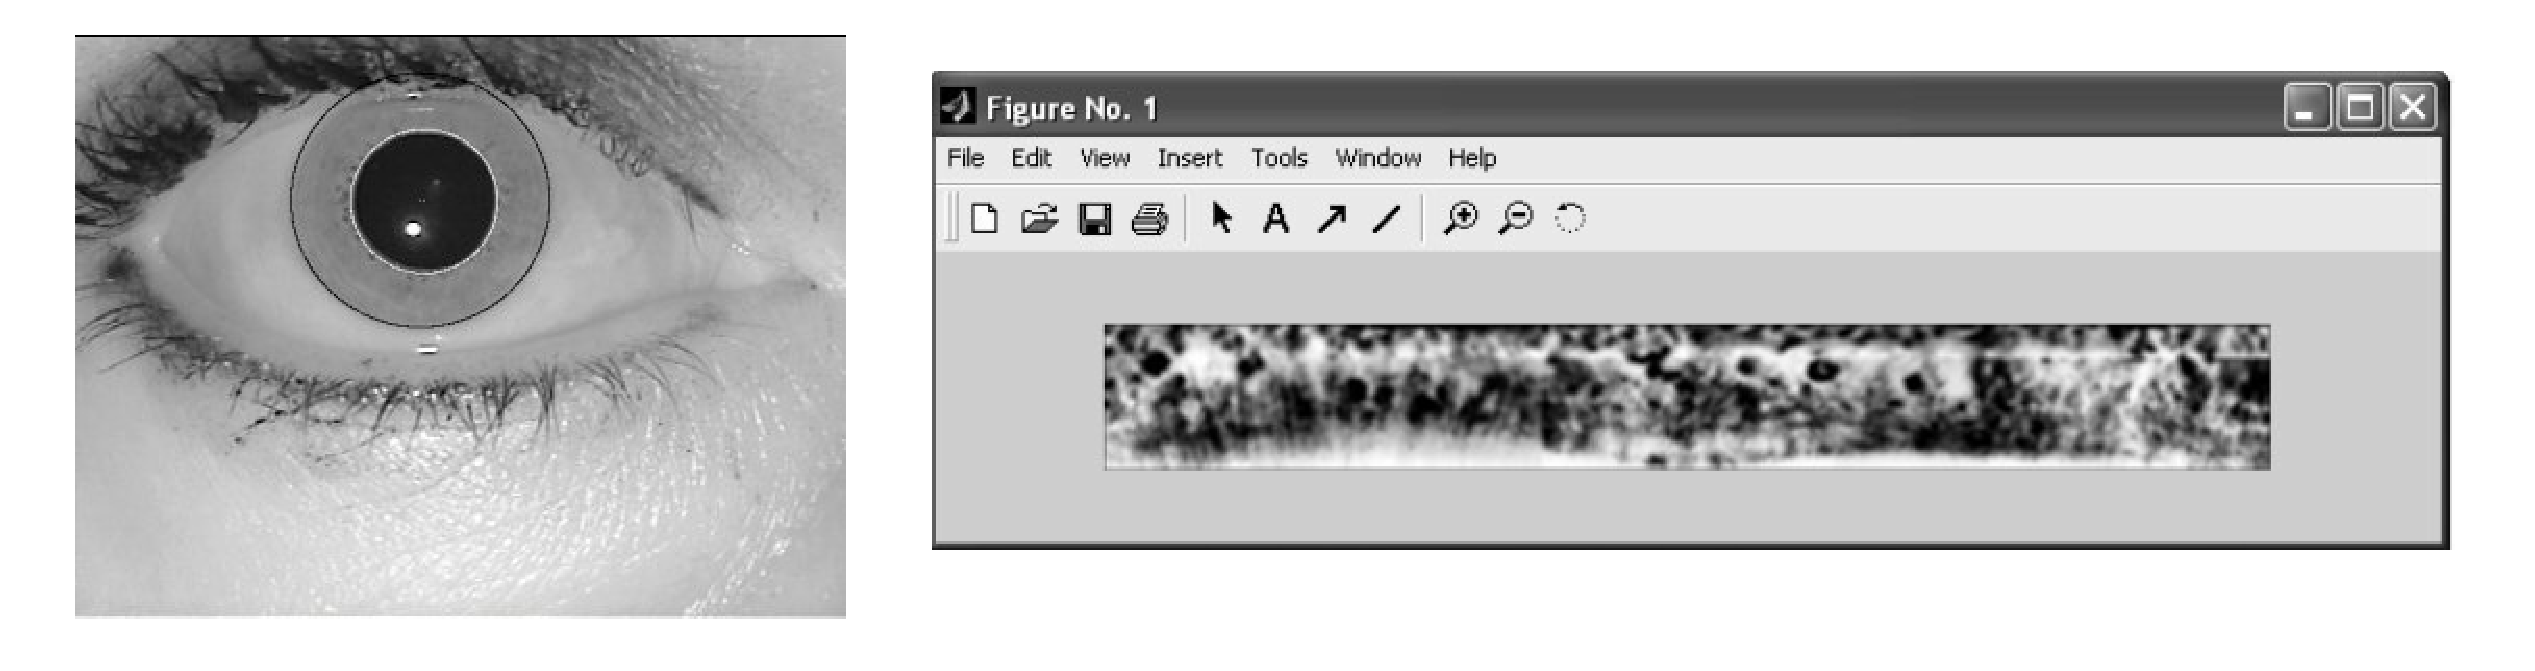
\includegraphics[width=17cm,angle=0]{images/iris/figura2.eps}

{\small\bf Figura 2. Segmentaci�n, transformaci�n polar e igualaci�n de histograma del iris de la izquierda.}
\end{figure}

\clearpage
\pagebreak


\bOpage{introcolor}{0.25}{TECNOLOG�A}

\begin{itemize}

\item {\bf Segmentaci�n}: los objetivos a lograr son la localizaci�n del
centro, eliminaci�n de la pupila y la escler�tica. Para hacer esto se
suele utilizar el hecho de que la pupila es negra y la escler�tica
blanca (figura 2, izquierda), mientras que el iris ocupa una tonalidad
intermedia. Ojo: todos los que hayan estudiado procesado de imagen
alguna vez saben que nunca es tan f�cil como decir, esto es negro,
aquello blanco... Estamos tratando con im�genes que tienen 256 niveles
de gris y lo primero que haremos ser� establecer dos umbrales (blanco
cuando el p�xel tiene un valor>u1, negro cuando tiene un
valor<u2). Con eso deber�amos tener una primera aproximaci�n, esto es:
un objeto similar a una corona circular que no es blanco ni negro pero
que est� rodeado por un objeto blanco y que rodea a un c�rculo
negro. Aplicando un poco de geometr�a deber�amos lograrlo. Otra fuente
de informaci�n que se puede usar a veces es el hecho de que el iris es
una zona con color (no sabemos cu�l pero tiene una tonalidad) mientras
que el resto de la foto es gris m�s claro (hasta el blanco) o m�s
oscuro (hasta el negro). A veces, aqu� tambi�n se puede utilizar
informaci�n de color ya que los puntos del iris tienen una tonalidad
que su entorno no posee (porque es blanco o negro... en definitiva es
gris m�s o menos brillante). 

\item {\bf Transformaci�n polar}: el iris es una corona circular y esa
no es una forma muy adecuada para trabajar. El objetivo es
``estirarlo'' para convertirlo en un rect�ngulo. Para eso haremos una
transformaci�n de coordenadas: cada punto tendr� dos coordenadas
polares (�ngulo $\theta$ y radio $\rho$). Si representamos de nuevo la
imagen pero llevando los �ngulos al eje x y el radio al eje y
lograremos un patr�n rectangular (figura 2, derecha). 

\item {\bf Normalizaci�n}: toda imagen capturada por una c�mara est�
sujeta a variaciones de iluminaci�n. Para evitar que eso cause
problemas debemos transformar la imagen para tener siempre el mismo
contraste (la diferencia entre el punto m�s oscuro y el m�s
claro). Una de las normalizaciones m�s utilizadas es la ``igualaci�n
de histograma'' que consiste en transformar algunos de los niveles de
gris en otros de forma que el histograma (el n�mero de veces que se
repite cada nivel) sea casi constante. 

\item {\bf Extracci�n de caracter�sticas texturales}: ahora se trata de
convertir la textura en un vector de n�meros. Para eso suelen usarse
los llamados filtros direccionales. Un ejemplo simple de filtro
direccional es el gradiente. Aplic�ndolo en una textura nos dar�a una
idea de la direcci�n de las l�neas en cada punto (el vector gradiente
saldr�a perpendicular a la direcci�n dominante). para extraer
caracter�sticas de texturas se suelen usar los filtros de Gabor. En la
t�cnica de Daugman (patentada) se procede a la cuantificaci�n de la
fase que resulta de la aplicaci�n de filtros Gabor complejos. La fase
de cada resultado local se codifica con 2 bits y cada iris queda
codificado con 2048 bits. Otras t�cnicas utilizan filtros paso-banda
ligeramente diferentes a los de Gabor y obtienen vectores reales en
lugar de codificaci�n binaria de la fase. 

\item {\bf Comparaci�n de los vectores codificados}: distancia de Hamming
(n�mero de bits diferentes) en la t�cnica de Daugman o distancias
matem�ticas cl�sicas (eucl�dea, norma 1, norma 2 ...) en los otros
casos. 

\end{itemize}

\begin{entradilla}
{\em El proceso de reconocimiento se reduce finalmente a la
{\color{introcolor}comparaci�n de los vectores obtenidos tras la cuantificaci�n de la fase}
del resultado de la aplicaci�n de los filtros de Gabor}
\end{entradilla}


\sectiontext{white}{black}{PARA SABER M�S}

S� lo que pod�is estar pensando... la explicaci�n anterior tiene una
``densidad similar al hormig�n'', sobre todo para lectores que no
compartan mi formaci�n (ingenier�a de telecomunicaci�n). En
fin... hablar de procesado de imagen a nivel t�cnico es lo que
tiene. Si alguien es ``muy cafetero'' o ``muy masoquista'' puede
ampliar datos con la siguiente bibliograf�a: 

\begin{itemize}
\item En la segmentaci�n habl� de elegir dos umbrales pero no dije
c�mo. Por prueba y error se pueden ajustar umbrales fijos. Tambi�n se
puede intentar calcularlos autom�ticamente. Existen innumerables
publicaciones sobre c�lculo de umbrales. La m�s cl�sica es el art�culo
de N. Otsu ``A Threshold Selection Method for Gray Level Histograms''
(publicado en la revista IEEE Transactions on System, Man and
Cybernetics en enero de 1979). Una referencia de infinitamente menor
calado pero que habla de obtener varios umbrales al mismo tiempo es el
art�culo ``Analysis Tools for Gray Level Histograms'' (publicado en el
congreso SPPRA-2003 en junio de 2003). S�, s�, una vez m�s me he
referenciado a m� mismo (copia en www.gpi.tsc.uvigo.es). 

\item La igualaci�n de histograma y, m�s en general, el uso de
histogramas en procesado de imagen es una t�cnica cl�sica explicada en
todos los libros de esta disciplina. Por ejemplo, os recomiendo
``Fundamentals of Digital Image Processing'' de A.K. Jain
(Prentice-Hall) o ``Digital Image Processing'' de R.C. Gonz�lez
(tambi�n editado por Prentice Hall). 

\end{itemize}

\ebOpage{introcolor}{0.25}{TECNOLOG�A}

\begin{itemize}
\item Para los filtros de Gabor he visto que hay un resumen
cualitativo correcto en la wikipedia
({\small \verb!http://es.wikipedia.org/wiki/Filtro_de_Gabor!}). Para mayores
profundidades hay tutoriales en la red como: 
\begin{itemize}
\item {\small \verb!http://mplab.ucsd.edu/wordpress/tutorials!\\\verb!/gabor.pdf!}.
\item {\small \verb!http://www.cs.rug.nl/~imaging/!\\\verb!simplecell.html!}.

Por cierto, no viene mucho al caso, pero Dennis Gabor tambi�n invent�
los hologramas y recibi� por ello el Premio Nobel de f�sica. Adem�s,
public� un curios�simo art�culo titulado ``Theory of Communication''
publicado por el IEEE en 1946 donde se propone una teor�a de la
informaci�n diferente a la de Shannon. 

\end{itemize}

\item Queda un poco como el villano de la historia, pero J.C. Daugman
fue el que resolvi� de una vez por todas el problema del
reconocimiento de iris (l�stima que no quisiera compartirlo). Su
trabajo est� descrito en varios art�culos. Por ejemplo, �ste lo
escribi� �l mismo y se puede bajar de internet:

{\small \verb!http://www.argus-solutions.com/pdfs/!\\\verb!recog_persons_iris.pdf!. }

���Ojo!!!
Que est� publicado no quiere decir que se puedan usar sus ideas sin
pagarle, tambi�n est� patentado (US Patent No. 4641349), Daugman fund�
la empresa Iridian Technologies para explotar esta
patente. Bueno... hasta donde yo s�, si en Europa no hay patentes
intelectuales podr�amos hacer productos usando este algortimo sin
mayor problema. �Alg�n abogado me puede corregir? A la hora de
comercializar esos productos en Estados Unidos s� que �bamos a tener
l�o... De todas formas no pienso intentarlo, no vaya a ser que tenga
que escribir el pr�ximo art�culo desde Carabanchel. 

\item En nuestra Escuela algo se ha trabajado sobre este tema. El
Proyecto Fin de Carrera ``Desarrollo de un Algoritmo de Identificaci�n
de Personas Mediante su Iris'' consiste en la implementaci�n en matlab
de un m�todo de reconocimiento (distinto al de Daugman). Su autor es
�scar Gonz�lez Rey y su tutor el profesor Jos� Luis Alba Castro. 

\end{itemize}

\sectiontext{white}{black}{ENSUCI�NDONOS LAS MANOS}

Yo, como todos, tiendo a la ley del m�nimo esfuerzo, por eso quer�a
dar por terminado este art�culo. La direcci�n de la revista, muy
sabiamente, me convenci� de que trabajara un poco m�s.... y aqu� est�
el resultado. He hecho un peque�o programa en matlab intentando poner
en pr�ctica parte de lo que os he contado.... A la izquierda el
c�digo, a la derecha los resultados parciales. ���Ojo!!! falta la
�ltima parte. 

\end{multicols}


\begin{multicols}{2}

\lstset{language=Matlab,framesep=5pt,basicstyle=\scriptsize}   
\begin{lstlisting}
%
% Extraccion de iris.
%
clear;close all; % Limpiar
fichero = 'Ojo1.jpg'; % Fichero de entrada
ImOjoRGB = imread(fichero); % Leer imagen
ImOjoHSV = rgb2hsv(ImOjoRGB); % Pasar a HSV
ImAux = imcomplement(ImOjoHSV(:,:,3)); % Negativo
ImDisc1 = ImAux.*ImOjoHSV(:,:,2);
% Iris = Poca luminacia y mucha saturacion
umbral = graythresh(ImDisc1);
% Umbral de saturacion (Otsu)
Masc0 = im2bw(ImDisc1,umbral); % Mascara previa
radio = 20;
ee = strel('disk',radio);
Masc1 = imopen(imfill(Masc0,'holes'),ee);
% Limpiar (empezamos eliminando la esclerotica)
% Ahora vamos a recortar el iris
[label,num] = bwlabel(Masc1);
% Etiquetar (separar objetos)
props = regionprops(label,'basic');
maxarea = -1;
idx = -1;
for i=1:num,
    % Buscar area maxima
    area = props(i).Area;
    if (area>maxarea)
        maxarea = area;
        idx = i;
    end
end
Rect = props(idx).BoundingBox;
IrisRGB = imcrop(ImOjoRGB,Rect);
IrisHSV = imcrop(ImOjoHSV,Rect);
ImDisc2 = imcrop(ImDisc1,Rect);
Masc2 = imcrop(Masc1, Rect);
% Recortar la zona de interes de cada imagen
%
% Ahora eliminar la pupila
IrisBN = rgb2gray(IrisRGB); % Pasar a B/N
U1 = 10;
U2 = 90; % Umbrales <<fijos>>
Masc3 = roicolor(IrisBN,U1,U2); % Mascara

\end{lstlisting}


\columnbreak
\begin{center}
\myfig{0}{images/iris/inicial.eps}{0.40}
\begin{center}
\begin{spacing}{0.3}
{\scriptsize Imagen Original}
\end{spacing}
\end{center}
\myfig{0}{images/iris/Fig01.eps}{0.40}
\begin{spacing}{0.3}
{\scriptsize {Imagen ``discriminante'': resultado de multiplicar la
saturaci�n (pureza del color) por el negativo del brillo (el iris
tiene mucha pureza de color y menos brillo que el resto de la
imagen).}}
\end{spacing}
\myfig{0}{images/iris/Fig02.eps}{0.3}
\begin{spacing}{0.3}
{\scriptsize M�scara del iris: se obtiene procesando la imagen anterior. Primero se rellenan las regiones con huecos, se limpia un poco y conservamos la mayor mancha blanca.}
\end{spacing}
\myfig{0}{images/iris/Fig03.eps}{0.3}
\begin{center}
\begin{spacing}{0.3}
{\scriptsize Iris recortado: la m�scara anterior nos permite eliminar la escler�tica... todav�a falta quitar la pupila.}
\end{spacing}
\end{center}
\end{center}
\end{multicols}

\clearpage
\pagebreak

\msection{introcolor}{black}{0.25}{TECNOLOG�A}

\begin{multicols}{2}

\lstset{language=Matlab,framesep=5pt,basicstyle=\small}   
\begin{lstlisting}
%
% Coger, de nuevo, la mayor area.
[label,num] = bwlabel(Masc3);
props = regionprops(label,'basic');
maxarea = -1;
idx = -1;
for i=1:num,
    area = props(i).Area;
    if (area>maxarea)
        maxarea = area;
        idx = i;
    end
end % Encontrar el area mayor
Masc3 = (label==idx);
Centro = props(idx).Centroid;
Xc = round(Centro(1));
Yc = round(Centro(2));
% Posicion del centro
radio = 10;
ee = strel('disk',radio);
Masc4 = imclose(Masc3,ee);
% Limpiar (rellenar huecos)
Imaux = double(imfill(Masc4,[Yc Xc]));
Masc5 = logical(Imaux-double(Masc4));
% Esta es la pupila
Imaux = double(imfill(Masc4,'holes'));
Masc6 = logical(Imaux-double(Masc5));
% Mascara rellena menos la pupila
%
% Ahora convertir el iris a un rectangulo.
props = regionprops(Masc5,'basic');
Centro = props(idx).Centroid;
Xc = round(Centro(1));
Yc = round(Centro(2));
% La mascara solo tiene un objeto
[alto,ancho] = size(Masc5);
Rmax = sqrt(alto^2+ancho^2)/2;
IrisCartesiano = [];
for tita=0:359, % Para cada angulo
  % Recorremos ese radio de la imagen.
  columna = [];
  for radio=0:Rmax,
    x = round(Xc+radio*cos(tita*pi/180));
    y = round(Yc+radio*sin(tita*pi/180));
    if (x>1)&(x<=ancho)&...
      (y>1)&(y<=alto)&...
      (Masc6(y,x)~=0)
        % Copiar punto en su nueva posicion
        valor = IrisBN(y,x);
    else
         % No hay punto para copiarlo
         valor = 0;
    end
    columna = [columna; valor];
  end
  IrisCartesiano = [IrisCartesiano columna];
end
%
% Ahora ecualizar el histograma
IrisNorm = histeq(IrisCartesiano);
% Esto ya lo hace el matlab por nosotros

\end{lstlisting}


\columnbreak

\begin{center}
\myfig{0}{images/iris/Fig04.eps}{0.65}
\begin{spacing}{0.3}
{\scriptsize {Histograma de grises del iris recortado: aqu� deber�amos encontrar los umbrales para localizar el iris. Funciona casi cualquier par que empiece despu�s del pico en cero (pupila negra) y acabe antes del pico en trono al 255 (restos de escler�tica).}}
\end{spacing}
\myfig{0}{images/iris/Fig05.eps}{0.35}
\begin{spacing}{0.3}
{\scriptsize M�scara inicial para eliminar la pupila.}
\end{spacing}
\myfig{0}{images/iris/Fig06.eps}{0.35}
\begin{spacing}{0.3}
{\scriptsize M�scara despu�s de limpiarla.}
\end{spacing}
\myfig{0}{images/iris/Fig07.eps}{0.35}
\begin{spacing}{0.3}
{\scriptsize Pupila localizada: hueco que contiene al centroide de la m�scara total.}
\end{spacing}

\myfig{0}{images/iris/Fig08.eps}{0.35}
\begin{spacing}{0.3}
{\scriptsize Si tenemos la pupila podemos rellenar toda la m�scara, EXCEPTO, la pupila.}
\end{spacing}

\myfig{0}{images/iris/Fig09.eps}{0.65}
\begin{spacing}{0.3}
{\scriptsize Iris rectangular: se obtiene recorriendo el iris mediante las coordenadas polares. Falta un ``trozo'' debido a que el p�rpado tapa casi medio iris.}
\end{spacing}

\myfig{0}{images/iris/Fig10.eps}{0.65}
\begin{spacing}{0.3}
{\scriptsize Iris normalizado: al aplicar la ecualizaci�n logramos repartir los niveles de gris y ganamos contraste. Ojo, realmente antes de esto habr�a que quitar la zona negra arriba y abajo y seguramente reescalar a un tama�o fijo.}
\end{spacing}
\end{center}
\end{multicols}


\clearpage
\pagebreak


% Este fichero es parte del N�mero 3 de la Revista Occam's Razor
% Revista Occam's Razor N�mero 3
%
% (c)  2007, 2008, 2009, The Occam's Razor Team
%
% Esta obra est� bajo una licencia Reconocimiento 3.0 Espa�a de
% Creative Commons. Para ver una copia de esta licencia, visite
% http://creativecommons.org/licenses/by/3.0/es/ o envie una carta a
% Creative Commons, 171 Second Street, Suite 300, San Francisco,
% California 94105, USA. 

%
% Secci�n Trucos


\rput(3,-2.5){\resizebox{!}{6cm}{{\epsfbox{images/general/varita3.eps}}}}
\begin{flushright}
\msection{red}{black}{0.1}{TRUCOS}

\mtitle{6cm}{Con un par... de l�neas}

\msubtitle{8cm}{Chuletillas para hacer cosas m� r�pido}

{\sf por Tamariz el de la Perd�z}

{\psset{linecolor=black,linestyle=dotted}\psline(-10,0)}

\end{flushright}

\vspace{4mm}

\begin{multicols}{2}
\raggedcolumns


\sectiontext{white}{black}{L�NEA DE COMANDOS AVANZADA PARA CUALQUIER
PROGRAMA DE CONSOLA}
\hrule
\vspace{2mm}

Utilizando la herramienta {\tt cle} podemos a�adir funcionalidades
avanzadas de edici�n a cualquier programa en modo consola.

Probad, por ejemplo (previa instalaci�n del paquete claro):

\vspace{2mm}

\hrule
{\footnotesize
\begin{verbatim}
occam@razor # cle nc localhost 110
\end{verbatim}
}
\hrule

\vspace{2mm}

Ahora, tras escribir unos comandos, pulsad el cursor arriba, o la
tecla inicio para editar la l�nea actual que est�is editando... Impresionante!.


\sectiontext{white}{black}{CIFRANDO TU NUEVO DISCO}
\hrule
\vspace{2mm}

Los ``device mappers'' proporcionados por los kernel Linux 2.6
permiten hacer cosas bastante interesantes. Una de ellas es el cifrado
de dispositivos de una forma sencilla. Si has instalado una
distribuci�n recientemente, esto funcionar� directamente, sino,
tendr�s que instalar algunos paquetes para poder utilizar los ``device mappers''.

\vspace{2mm}
\hrule
{\footnotesize
\begin{verbatim}
occam@razor # cfisk /dev/sdb
occam@razor # crypsetup create -y crypt /dev/sdb1 
Password:
Password:
occam@razor # mfs.ext3 /dev/mapper/crypt
occam@razor # mount /dev/mapper/crypt \
> /mnt/mi_disco_seguro
occam@razor #
\end{verbatim}		   
}
\hrule
\vspace{2mm}

La secuencia de comandos anterior nos permite formatear el disco duro
(cfdisk), activar el device mapper para una de las particiones
(cryptsetuo) formatearla (mkfs.ext3) y montar la nueva partici�n cifrada.

Eso solo lo ten�is que hacer la primera vez. Para su uso normal solo ten�is que hacer lo siguiente:

\vspace{2mm}
\hrule
{\footnotesize
\begin{verbatim}
occam@razor # crypsetup create crypt /dev/sdb1 
occam@razor # mount /dev/mapper/crypt \
> /mnt/mi_disco_seguro
occam@razor #
\end{verbatim}		   
}
\hrule
\vspace{2mm}



\sectiontext{white}{black}{VOLCADO HEXADECIMAL}
\hrule
\vspace{2mm}

La herramienta {\tt od} es una de esas grandes desconocidas en los
sistemas UNIX, que merece la pena conocer dada su
versatilidad. B�sicamente, esta herramienta nos permite realizar
volcados de datos binarios.

Probablemente los par�metros que utilic�is m�s a menudo ser�n estos:

\vspace{2mm}

\hrule
{\scriptsize
\begin{verbatim}
occams@razor # od -Ax -tx1z /bin/ls
\end{verbatim}
}
\hrule
\vspace{2mm}

El primer par�metro -Ax indica que la base del volcado ser�
hexadecimal (otros valores posibles son d para decimal y o para
octal). A continuaci�n indicamos el formato deseado para el volcado,
en este caso {\tt x1z} es la cadena elegida. En ella, {\tt x1} indica
a od que vuelque cada l�nea de datos como valores hexadecimales de 1
byte. Si os interesa, por lo que sea, buscar valores de 16 � 32 bits
en vuestro chorro binario cambiad 1 por 2 � 4. La {\tt z} final indica
a od que, adem�s, vuelque esos datos como una cadena de caracteres.

\vspace{2mm}

\hrule
{\scriptsize
\begin{verbatim}
occams@razor # nc servicio 10000 | od -Ax -tx1z /bin/ls
\end{verbatim}
}
\hrule
\vspace{2mm}

Cuando no hay otra cosa a mano, es una opci�n para depurar protocolos
binarios :).

\vspace{2mm}

\sectiontext{white}{black}{CIFRADO DE FICHEROS}
\hrule
\vspace{2mm}

Cifrar ficheros es realmente sencillo usando gpg. Alguna gente cree
que para usar gpg tiene que generar distintos tipos de claves que no
sabe muy bien como manejar... Bien, eso es cierto, para utilizar toda
la potencia de gpg, pero si solo quieres cifrar un fichero, gpg ofrece
un modo de cifrado sim�trico... el de la palabra secreta de toda la
vida.

Lo �nico que ten�is que hacer para cifrar y posteriormente descifrar
un fichero es: 

\vspace{2mm}

\hrule
{\scriptsize
\begin{verbatim}
occams@razor $ gpg -c mi_fichero.tgz
occams@razor $ gpg  mi_fichero.tgz.gpg
\end{verbatim}
}
\hrule 
\vspace{2mm}

Por defecto, gpg usa el algoritmo CAST5, pero pod�is utilizar
cualquiera disponible en vuestra versi�n. Para saber que algoritmos
pod�is usar:


\vspace{2mm}

\hrule
{\scriptsize
\begin{verbatim}
occams@razor $ gpg --version
(...)
Supported algorithms:
Pubkey: RSA, RSA-E, RSA-S, ELG-E, DSA
Cypher: 3DES, CAST5, BLOWFISH, AES, AES192, AES256, TWOFISH
Hash: MD5, SHA1, RIPEMD160, SHA256, SHA384, SHA512
Compression: Uncompressed, ZIP, ZLIB, BZIP2
occams@razor $
\end{verbatim}
}
\hrule 
\vspace{2mm}

Como pod�is ver, DES ya ni aparece :)

%% Call for tricks

\vspace{2mm}

\sectiontext{white}{black}{UNDO EN VIM}
\hrule
\vspace{2mm}

S�, se nos olvid� comentarlo en el art�culo y ya no ten�amos
sitio. Pulsad ``u'' en modo comando para deshacer y ``CTRL+R'' para
rehacer. ;)

\vspace{2mm}

\colorbox{introcolor}{
\begin{minipage}{.9\linewidth}{
\textbf{\textsf{Env�a tus trucos}}

\vspace{1mm}

\textsf{Puedes enviarnos esos trucos que usas a diario para compartirlos con el resto de lectores a la direcci�n: }

\vspace{2mm}

\texttt{occams-razor@uvigo.es}
}
\end{minipage}
}

\raggedcolumns
\pagebreak

\vspace{6cm}
\end{multicols}

\clearpage
\pagebreak


% Este fichero es parte del N�mero 3 de la Revista Occam's Razor
% Revista Occam's Razor N�mero 3
%
% (c)  2007, 2008, The Occam's Razor Team
%
% Esta obra est� bajo una licencia Reconocimiento 2.5 Espa�a de Creative
% Commons. Para ver una copia de esta licencia, visite 
% http://creativecommons.org/licenses/by/2.5/es/
% o envie una carta a Creative Commons, 171 Second Street, Suite 300, 
% San Francisco, California 94105, USA.

\pagestyle{empty}
\rput(8,-14){\epsfbox{images/cfp.eps}}

\pagebreak

\rput(8,-14){\epsfbox{images/contraportada.eps}}

\pagebreak


\end{document}
